\documentclass[]{article}
\usepackage{lmodern}
\usepackage{amssymb,amsmath}
\usepackage{ifxetex,ifluatex}
\usepackage{fixltx2e} % provides \textsubscript
\ifnum 0\ifxetex 1\fi\ifluatex 1\fi=0 % if pdftex
  \usepackage[T1]{fontenc}
  \usepackage[utf8]{inputenc}
\else % if luatex or xelatex
  \ifxetex
    \usepackage{mathspec}
  \else
    \usepackage{fontspec}
  \fi
  \defaultfontfeatures{Ligatures=TeX,Scale=MatchLowercase}
\fi
% use upquote if available, for straight quotes in verbatim environments
\IfFileExists{upquote.sty}{\usepackage{upquote}}{}
% use microtype if available
\IfFileExists{microtype.sty}{%
\usepackage{microtype}
\UseMicrotypeSet[protrusion]{basicmath} % disable protrusion for tt fonts
}{}
\usepackage[margin=1in]{geometry}
\usepackage{hyperref}
\hypersetup{unicode=true,
            pdftitle={Dormancy and dispersal structure bacterial communities across ecosystem boundaries},
            pdfauthor={Nathan I. Wisnoski, Mario E. Muscarella, Megan L. Larsen, and Jay T. Lennon},
            pdfborder={0 0 0},
            breaklinks=true}
\urlstyle{same}  % don't use monospace font for urls
\usepackage{color}
\usepackage{fancyvrb}
\newcommand{\VerbBar}{|}
\newcommand{\VERB}{\Verb[commandchars=\\\{\}]}
\DefineVerbatimEnvironment{Highlighting}{Verbatim}{commandchars=\\\{\}}
% Add ',fontsize=\small' for more characters per line
\usepackage{framed}
\definecolor{shadecolor}{RGB}{248,248,248}
\newenvironment{Shaded}{\begin{snugshade}}{\end{snugshade}}
\newcommand{\KeywordTok}[1]{\textcolor[rgb]{0.13,0.29,0.53}{\textbf{#1}}}
\newcommand{\DataTypeTok}[1]{\textcolor[rgb]{0.13,0.29,0.53}{#1}}
\newcommand{\DecValTok}[1]{\textcolor[rgb]{0.00,0.00,0.81}{#1}}
\newcommand{\BaseNTok}[1]{\textcolor[rgb]{0.00,0.00,0.81}{#1}}
\newcommand{\FloatTok}[1]{\textcolor[rgb]{0.00,0.00,0.81}{#1}}
\newcommand{\ConstantTok}[1]{\textcolor[rgb]{0.00,0.00,0.00}{#1}}
\newcommand{\CharTok}[1]{\textcolor[rgb]{0.31,0.60,0.02}{#1}}
\newcommand{\SpecialCharTok}[1]{\textcolor[rgb]{0.00,0.00,0.00}{#1}}
\newcommand{\StringTok}[1]{\textcolor[rgb]{0.31,0.60,0.02}{#1}}
\newcommand{\VerbatimStringTok}[1]{\textcolor[rgb]{0.31,0.60,0.02}{#1}}
\newcommand{\SpecialStringTok}[1]{\textcolor[rgb]{0.31,0.60,0.02}{#1}}
\newcommand{\ImportTok}[1]{#1}
\newcommand{\CommentTok}[1]{\textcolor[rgb]{0.56,0.35,0.01}{\textit{#1}}}
\newcommand{\DocumentationTok}[1]{\textcolor[rgb]{0.56,0.35,0.01}{\textbf{\textit{#1}}}}
\newcommand{\AnnotationTok}[1]{\textcolor[rgb]{0.56,0.35,0.01}{\textbf{\textit{#1}}}}
\newcommand{\CommentVarTok}[1]{\textcolor[rgb]{0.56,0.35,0.01}{\textbf{\textit{#1}}}}
\newcommand{\OtherTok}[1]{\textcolor[rgb]{0.56,0.35,0.01}{#1}}
\newcommand{\FunctionTok}[1]{\textcolor[rgb]{0.00,0.00,0.00}{#1}}
\newcommand{\VariableTok}[1]{\textcolor[rgb]{0.00,0.00,0.00}{#1}}
\newcommand{\ControlFlowTok}[1]{\textcolor[rgb]{0.13,0.29,0.53}{\textbf{#1}}}
\newcommand{\OperatorTok}[1]{\textcolor[rgb]{0.81,0.36,0.00}{\textbf{#1}}}
\newcommand{\BuiltInTok}[1]{#1}
\newcommand{\ExtensionTok}[1]{#1}
\newcommand{\PreprocessorTok}[1]{\textcolor[rgb]{0.56,0.35,0.01}{\textit{#1}}}
\newcommand{\AttributeTok}[1]{\textcolor[rgb]{0.77,0.63,0.00}{#1}}
\newcommand{\RegionMarkerTok}[1]{#1}
\newcommand{\InformationTok}[1]{\textcolor[rgb]{0.56,0.35,0.01}{\textbf{\textit{#1}}}}
\newcommand{\WarningTok}[1]{\textcolor[rgb]{0.56,0.35,0.01}{\textbf{\textit{#1}}}}
\newcommand{\AlertTok}[1]{\textcolor[rgb]{0.94,0.16,0.16}{#1}}
\newcommand{\ErrorTok}[1]{\textcolor[rgb]{0.64,0.00,0.00}{\textbf{#1}}}
\newcommand{\NormalTok}[1]{#1}
\usepackage{longtable,booktabs}
\usepackage{graphicx,grffile}
\makeatletter
\def\maxwidth{\ifdim\Gin@nat@width>\linewidth\linewidth\else\Gin@nat@width\fi}
\def\maxheight{\ifdim\Gin@nat@height>\textheight\textheight\else\Gin@nat@height\fi}
\makeatother
% Scale images if necessary, so that they will not overflow the page
% margins by default, and it is still possible to overwrite the defaults
% using explicit options in \includegraphics[width, height, ...]{}
\setkeys{Gin}{width=\maxwidth,height=\maxheight,keepaspectratio}
\IfFileExists{parskip.sty}{%
\usepackage{parskip}
}{% else
\setlength{\parindent}{0pt}
\setlength{\parskip}{6pt plus 2pt minus 1pt}
}
\setlength{\emergencystretch}{3em}  % prevent overfull lines
\providecommand{\tightlist}{%
  \setlength{\itemsep}{0pt}\setlength{\parskip}{0pt}}
\setcounter{secnumdepth}{0}
% Redefines (sub)paragraphs to behave more like sections
\ifx\paragraph\undefined\else
\let\oldparagraph\paragraph
\renewcommand{\paragraph}[1]{\oldparagraph{#1}\mbox{}}
\fi
\ifx\subparagraph\undefined\else
\let\oldsubparagraph\subparagraph
\renewcommand{\subparagraph}[1]{\oldsubparagraph{#1}\mbox{}}
\fi

%%% Use protect on footnotes to avoid problems with footnotes in titles
\let\rmarkdownfootnote\footnote%
\def\footnote{\protect\rmarkdownfootnote}

%%% Change title format to be more compact
\usepackage{titling}

% Create subtitle command for use in maketitle
\newcommand{\subtitle}[1]{
  \posttitle{
    \begin{center}\large#1\end{center}
    }
}

\setlength{\droptitle}{-2em}

  \title{Dormancy and dispersal structure bacterial communities across ecosystem
boundaries}
    \pretitle{\vspace{\droptitle}\centering\huge}
  \posttitle{\par}
    \author{Nathan I. Wisnoski, Mario E. Muscarella, Megan L. Larsen, and Jay T.
Lennon}
    \preauthor{\centering\large\emph}
  \postauthor{\par}
      \predate{\centering\large\emph}
  \postdate{\par}
    \date{26 March, 2019}

\usepackage{array}
\usepackage{graphics}

\begin{document}
\maketitle

\section{Initial Setup}\label{initial-setup}

First, we'll load the packages we'll need for the analysis, as well as
some other functions.

\begin{Shaded}
\begin{Highlighting}[]
\CommentTok{# Import Required Packages}
\KeywordTok{library}\NormalTok{(}\StringTok{"png"}\NormalTok{)}
\KeywordTok{library}\NormalTok{(}\StringTok{"grid"}\NormalTok{)}
\KeywordTok{library}\NormalTok{(}\StringTok{"tidyverse"}\NormalTok{)   }
\KeywordTok{library}\NormalTok{(}\StringTok{"vegan"}\NormalTok{)}
\KeywordTok{library}\NormalTok{(}\StringTok{"xtable"}\NormalTok{)}
\KeywordTok{library}\NormalTok{(}\StringTok{"viridis"}\NormalTok{)}
\KeywordTok{library}\NormalTok{(}\StringTok{"cowplot"}\NormalTok{)}
\KeywordTok{library}\NormalTok{(}\StringTok{"adespatial"}\NormalTok{)}
\KeywordTok{library}\NormalTok{(}\StringTok{"ggrepel"}\NormalTok{)}
\KeywordTok{library}\NormalTok{(}\StringTok{"gganimate"}\NormalTok{)}
\KeywordTok{library}\NormalTok{(}\StringTok{"maps"}\NormalTok{)}
\KeywordTok{library}\NormalTok{(}\StringTok{"rgdal"}\NormalTok{)}
\KeywordTok{library}\NormalTok{(}\StringTok{"iNEXT"}\NormalTok{)}
\KeywordTok{library}\NormalTok{(}\StringTok{"officer"}\NormalTok{)}
\KeywordTok{library}\NormalTok{(}\StringTok{"flextable"}\NormalTok{) }\CommentTok{#must have gdtools installed also}
\KeywordTok{library}\NormalTok{(}\StringTok{"broom"}\NormalTok{)}
\KeywordTok{library}\NormalTok{(}\StringTok{"ggpmisc"}\NormalTok{)}
\KeywordTok{library}\NormalTok{(}\StringTok{"pander"}\NormalTok{)}
\KeywordTok{library}\NormalTok{(}\StringTok{"lubridate"}\NormalTok{)}

\KeywordTok{source}\NormalTok{(}\StringTok{"bin/mothur_tools.R"}\NormalTok{)}
\NormalTok{se <-}\StringTok{ }\ControlFlowTok{function}\NormalTok{(x, ...)\{}\KeywordTok{sd}\NormalTok{(x, }\DataTypeTok{na.rm =} \OtherTok{TRUE}\NormalTok{)}\OperatorTok{/}\KeywordTok{sqrt}\NormalTok{(}\KeywordTok{length}\NormalTok{(}\KeywordTok{na.omit}\NormalTok{(x)))\}}
\end{Highlighting}
\end{Shaded}

Next, we'll set the aesthetics of the figures we will produce.

\begin{Shaded}
\begin{Highlighting}[]
\NormalTok{my.cols <-}\StringTok{ }\NormalTok{RColorBrewer}\OperatorTok{::}\KeywordTok{brewer.pal}\NormalTok{(}\DataTypeTok{n =} \DecValTok{4}\NormalTok{, }\DataTypeTok{name =} \StringTok{"Greys"}\NormalTok{)[}\DecValTok{3}\OperatorTok{:}\DecValTok{4}\NormalTok{]}

\CommentTok{# Set theme for figures in the paper}
\KeywordTok{theme_set}\NormalTok{(}\KeywordTok{theme_classic}\NormalTok{() }\OperatorTok{+}\StringTok{ }
\StringTok{  }\KeywordTok{theme}\NormalTok{(}\DataTypeTok{axis.title =} \KeywordTok{element_text}\NormalTok{(}\DataTypeTok{size =} \DecValTok{16}\NormalTok{),}
        \DataTypeTok{axis.title.x =} \KeywordTok{element_text}\NormalTok{(}\DataTypeTok{margin =} \KeywordTok{margin}\NormalTok{(}\DataTypeTok{t =} \DecValTok{15}\NormalTok{, }\DataTypeTok{b =} \DecValTok{15}\NormalTok{)),}
        \DataTypeTok{axis.title.y =} \KeywordTok{element_text}\NormalTok{(}\DataTypeTok{margin =} \KeywordTok{margin}\NormalTok{(}\DataTypeTok{l =} \DecValTok{15}\NormalTok{, }\DataTypeTok{r =} \DecValTok{15}\NormalTok{)),}
        \DataTypeTok{axis.text =} \KeywordTok{element_text}\NormalTok{(}\DataTypeTok{size =} \DecValTok{14}\NormalTok{),}
        \DataTypeTok{axis.text.x =} \KeywordTok{element_text}\NormalTok{(}\DataTypeTok{margin =} \KeywordTok{margin}\NormalTok{(}\DataTypeTok{t =} \DecValTok{5}\NormalTok{)),}
        \DataTypeTok{axis.text.y =} \KeywordTok{element_text}\NormalTok{(}\DataTypeTok{margin =} \KeywordTok{margin}\NormalTok{(}\DataTypeTok{r =} \DecValTok{5}\NormalTok{)),}
        \CommentTok{#axis.line.x = element_line(size = 1),}
        \CommentTok{#axis.line.y = element_line(size = 1),}
        \DataTypeTok{axis.line.x =} \KeywordTok{element_blank}\NormalTok{(),}
        \DataTypeTok{axis.line.y =} \KeywordTok{element_blank}\NormalTok{(),}
        \DataTypeTok{axis.ticks.x =} \KeywordTok{element_line}\NormalTok{(}\DataTypeTok{size =} \DecValTok{1}\NormalTok{),}
        \DataTypeTok{axis.ticks.y =} \KeywordTok{element_line}\NormalTok{(}\DataTypeTok{size =} \DecValTok{1}\NormalTok{),}
        \DataTypeTok{axis.ticks.length =} \KeywordTok{unit}\NormalTok{(.}\DecValTok{1}\NormalTok{, }\StringTok{"in"}\NormalTok{),}
        \DataTypeTok{panel.border =} \KeywordTok{element_rect}\NormalTok{(}\DataTypeTok{color =} \StringTok{"black"}\NormalTok{, }\DataTypeTok{fill =} \OtherTok{NA}\NormalTok{, }\DataTypeTok{size =} \FloatTok{1.5}\NormalTok{),}
        \DataTypeTok{legend.title =} \KeywordTok{element_blank}\NormalTok{(),}
        \DataTypeTok{legend.text =} \KeywordTok{element_text}\NormalTok{(}\DataTypeTok{size =} \DecValTok{14}\NormalTok{),}
        \DataTypeTok{strip.text =} \KeywordTok{element_text}\NormalTok{(}\DataTypeTok{size =} \DecValTok{14}\NormalTok{),}
        \DataTypeTok{strip.background =} \KeywordTok{element_blank}\NormalTok{()}
\NormalTok{        ))}
\end{Highlighting}
\end{Shaded}

\subsection{Import Data}\label{import-data}

Here, we read in the processed sequence files from mothur (shared and
taxonomy) and a design of the sampling. We also load in the
environmental data. We then remove the mock community from the dataset
and ensure the the design and OTU table are aligned by row.

\begin{Shaded}
\begin{Highlighting}[]
\CommentTok{# Define Inputs}
\CommentTok{# Design = general design file for experiment}
\CommentTok{# shared = OTU table from mothur with sequence similarity clustering}
\CommentTok{# Taxonomy = Taxonomic information for each OTU}
\NormalTok{design <-}\StringTok{ "data/UL.design.txt"}
\NormalTok{shared <-}\StringTok{ "data/ul_resgrad.trim.contigs.good.unique.good.filter.unique.precluster.pick.pick.pick.opti_mcc.shared"}
\NormalTok{taxon  <-}\StringTok{ "data/ul_resgrad.trim.contigs.good.unique.good.filter.unique.precluster.pick.pick.pick.opti_mcc.0.03.cons.taxonomy"}

\CommentTok{# Import Design}
\NormalTok{design <-}\StringTok{ }\KeywordTok{read.delim}\NormalTok{(design, }\DataTypeTok{header=}\NormalTok{T, }\DataTypeTok{row.names=}\DecValTok{1}\NormalTok{)}

\CommentTok{# Import Shared Files}
\NormalTok{OTUs <-}\StringTok{ }\KeywordTok{read.otu}\NormalTok{(}\DataTypeTok{shared =}\NormalTok{ shared, }\DataTypeTok{cutoff =} \StringTok{"0.03"}\NormalTok{)    }\CommentTok{# 97% Similarity}

\CommentTok{# Import Taxonomy}
\NormalTok{OTU.tax <-}\StringTok{ }\KeywordTok{read.tax}\NormalTok{(}\DataTypeTok{taxonomy =}\NormalTok{ taxon, }\DataTypeTok{format =} \StringTok{"rdp"}\NormalTok{)}

\CommentTok{# Load environmental data}
\NormalTok{env.dat <-}\StringTok{ }\KeywordTok{read.csv}\NormalTok{(}\StringTok{"data/ResGrad_EnvDat.csv"}\NormalTok{, }\DataTypeTok{header =} \OtherTok{TRUE}\NormalTok{)}
\NormalTok{env.dat <-}\StringTok{ }\NormalTok{env.dat[}\OperatorTok{-}\DecValTok{16}\NormalTok{,]}

\CommentTok{# Subset to just the reservoir gradient sites}
\NormalTok{OTUs <-}\StringTok{ }\NormalTok{OTUs[}\KeywordTok{str_which}\NormalTok{(}\KeywordTok{rownames}\NormalTok{(OTUs), }\StringTok{"RG"}\NormalTok{),]}
\NormalTok{OTUs <-}\StringTok{ }\NormalTok{OTUs[}\OperatorTok{-}\KeywordTok{which}\NormalTok{(}\KeywordTok{rownames}\NormalTok{(OTUs) }\OperatorTok{==}\StringTok{ "RGMockComm"}\NormalTok{),]}

\CommentTok{# make sure OTU table matches up with design order}
\NormalTok{OTUs <-}\StringTok{ }\NormalTok{OTUs[}\KeywordTok{match}\NormalTok{(}\KeywordTok{rownames}\NormalTok{(design), }\KeywordTok{rownames}\NormalTok{(OTUs)),]}
\end{Highlighting}
\end{Shaded}

\subsection{Clean and transform OTU
table}\label{clean-and-transform-otu-table}

Here, we remove OTUs with low incidence across sites, we remove any
samples with low coverage, and we standardize the OTU table by
log-transforming the abundances and relativizing by site.

\begin{Shaded}
\begin{Highlighting}[]
\CommentTok{# Remove OTUs with less than two occurences across all sites}
\NormalTok{OTUs <-}\StringTok{ }\NormalTok{OTUs[, }\KeywordTok{which}\NormalTok{(}\KeywordTok{colSums}\NormalTok{(OTUs) }\OperatorTok{>=}\StringTok{ }\DecValTok{2}\NormalTok{)]}

\CommentTok{# Sequencing Coverage}
\NormalTok{coverage <-}\StringTok{ }\KeywordTok{rowSums}\NormalTok{(OTUs)}

\CommentTok{# Remove Low Coverage Samples (This code removes two sites: Site 5DNA, Site 6cDNA)}
\NormalTok{lows <-}\StringTok{ }\KeywordTok{which}\NormalTok{(coverage }\OperatorTok{<}\StringTok{ }\DecValTok{10000}\NormalTok{)}
\NormalTok{OTUs <-}\StringTok{ }\NormalTok{OTUs[}\OperatorTok{-}\KeywordTok{which}\NormalTok{(coverage }\OperatorTok{<}\StringTok{ }\DecValTok{10000}\NormalTok{), ]}
\NormalTok{design <-}\StringTok{ }\NormalTok{design[}\OperatorTok{-}\KeywordTok{which}\NormalTok{(coverage }\OperatorTok{<}\StringTok{ }\DecValTok{10000}\NormalTok{), ]}
\CommentTok{# Remove OTUs with less than two occurences across all sites}
\NormalTok{OTUs <-}\StringTok{ }\NormalTok{OTUs[, }\KeywordTok{which}\NormalTok{(}\KeywordTok{colSums}\NormalTok{(OTUs) }\OperatorTok{>=}\StringTok{ }\DecValTok{2}\NormalTok{)]}
\NormalTok{coverage <-}\StringTok{ }\KeywordTok{rowSums}\NormalTok{(OTUs)}
\KeywordTok{set.seed}\NormalTok{(}\DecValTok{47405}\NormalTok{)}
\NormalTok{OTUs <-}\StringTok{ }\KeywordTok{rrarefy}\NormalTok{(OTUs, }\KeywordTok{min}\NormalTok{(coverage))}

\CommentTok{# Make Relative Abundance Matrices}
\NormalTok{OTUsREL <-}\StringTok{ }\KeywordTok{decostand}\NormalTok{(OTUs, }\DataTypeTok{method =} \StringTok{"total"}\NormalTok{)}

\CommentTok{# Log Transform Relative Abundances}
\NormalTok{OTUsREL.log <-}\StringTok{ }\KeywordTok{decostand}\NormalTok{(OTUs, }\DataTypeTok{method =} \StringTok{"log"}\NormalTok{)}
\end{Highlighting}
\end{Shaded}

\section{Reservoir environmental
gradients}\label{reservoir-environmental-gradients}

Just to see if there are any strong underlying resource or nutrient
gradients in the reservoir, we'll plot them along the distance of the
reservoir.

\begin{Shaded}
\begin{Highlighting}[]
\NormalTok{facet.labs <-}\StringTok{ }\KeywordTok{c}\NormalTok{(}\StringTok{`}\DataTypeTok{chla}\StringTok{`}\NormalTok{ =}\StringTok{ "Chlorophyll-a"}\NormalTok{,}
                \StringTok{`}\DataTypeTok{color}\StringTok{`}\NormalTok{ =}\StringTok{ "Color"}\NormalTok{,}
                \StringTok{`}\DataTypeTok{DO}\StringTok{`}\NormalTok{ =}\StringTok{ "Dissolved Oxygen"}\NormalTok{,}
                \StringTok{`}\DataTypeTok{pH}\StringTok{`}\NormalTok{ =}\StringTok{ "pH"}\NormalTok{,}
                \StringTok{`}\DataTypeTok{TP}\StringTok{`}\NormalTok{ =}\StringTok{ "Total Phosphorus"}\NormalTok{)}

\NormalTok{env.dat }\OperatorTok\StringTok{ }\KeywordTok{select}\NormalTok{(dist.dam, DO, pH, TP, chla) }\OperatorTok\StringTok{ }
\StringTok{  }\KeywordTok{gather}\NormalTok{(variable, value, }\OperatorTok{-}\NormalTok{dist.dam) }\OperatorTok\StringTok{ }
\StringTok{  }\KeywordTok{ggplot}\NormalTok{(}\KeywordTok{aes}\NormalTok{(}\DataTypeTok{x =}\NormalTok{ dist.dam, }\DataTypeTok{y =}\NormalTok{ value)) }\OperatorTok{+}\StringTok{ }
\StringTok{  }\KeywordTok{geom_point}\NormalTok{() }\OperatorTok{+}\StringTok{ }
\StringTok{  }\KeywordTok{geom_smooth}\NormalTok{(}\DataTypeTok{method =} \StringTok{"lm"}\NormalTok{, }\DataTypeTok{color =} \StringTok{"black"}\NormalTok{) }\OperatorTok{+}\StringTok{ }
\StringTok{  }\KeywordTok{facet_grid}\NormalTok{(variable }\OperatorTok{~}\NormalTok{., }\DataTypeTok{scales =} \StringTok{"free"}\NormalTok{, }\DataTypeTok{switch =} \StringTok{"y"}\NormalTok{, }
             \DataTypeTok{labeller =} \KeywordTok{as_labeller}\NormalTok{(facet.labs)) }\OperatorTok{+}\StringTok{ }
\StringTok{  }\KeywordTok{theme}\NormalTok{(}\DataTypeTok{strip.background =} \KeywordTok{element_blank}\NormalTok{(), }
        \DataTypeTok{strip.text =} \KeywordTok{element_text}\NormalTok{(}\DataTypeTok{size =} \DecValTok{14}\NormalTok{),}
        \DataTypeTok{strip.placement =} \StringTok{"outside"}\NormalTok{) }\OperatorTok{+}\StringTok{ }
\StringTok{  }\KeywordTok{labs}\NormalTok{(}\DataTypeTok{x =} \StringTok{"Reservoir distance (m)"}\NormalTok{,}
       \DataTypeTok{y =} \StringTok{""}\NormalTok{) }\OperatorTok{+}
\StringTok{  }\KeywordTok{scale_x_reverse}\NormalTok{() }\OperatorTok{+}
\StringTok{  }\KeywordTok{scale_y_continuous}\NormalTok{()}
\end{Highlighting}
\end{Shaded}

\begin{center}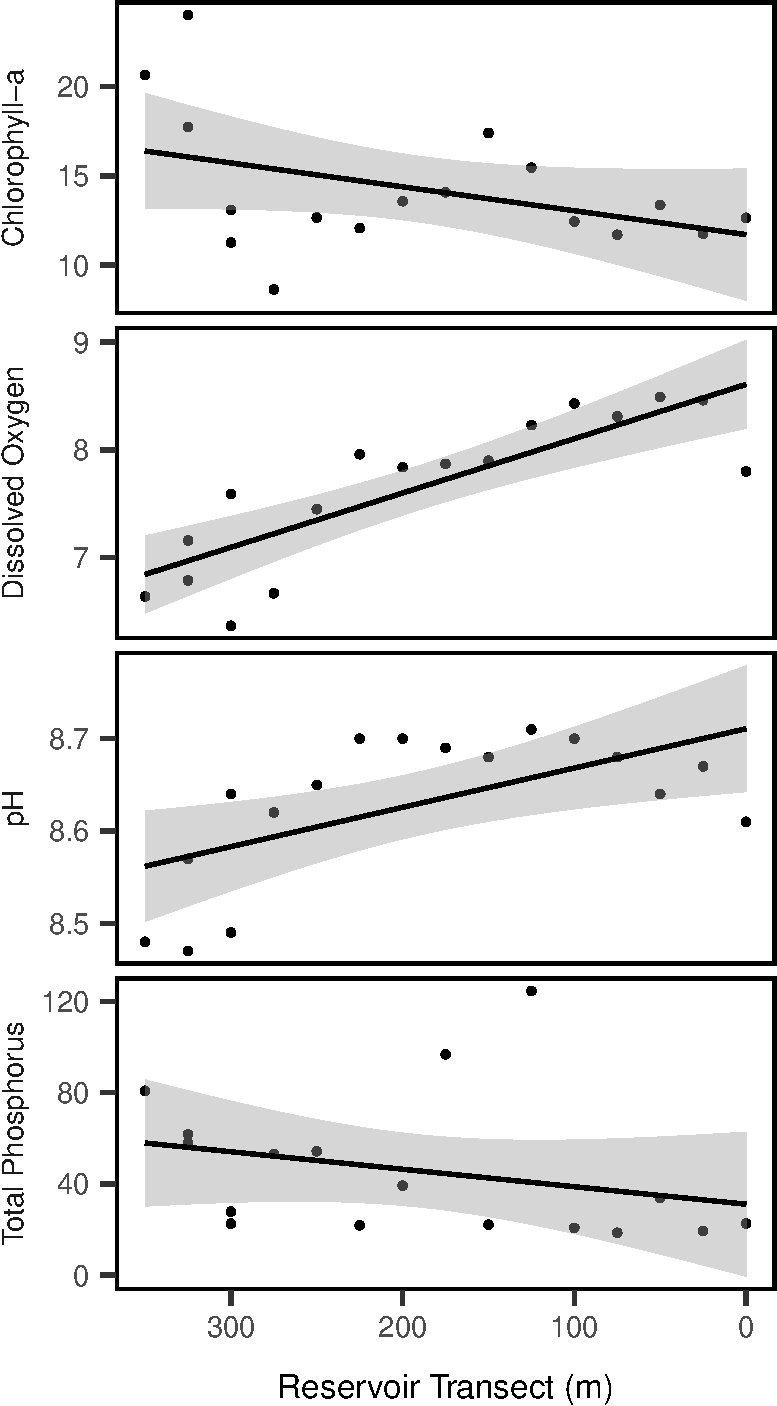
\includegraphics{ReservoirGradient_files/figure-latex/env_plot-1} \end{center}

So, there are some weak gradients, but nothing too prevailing.

\section{Analyze Diversity}\label{analyze-diversity}

Now, we will analyze the bacterial diversity in the reservoir and nearby
soils to figure out how well they support different mechanisms of
community assembly.

\subsection{\texorpdfstring{How does \(\alpha\)-diversity vary along the
reservoir?}{How does \textbackslash{}alpha-diversity vary along the reservoir?}}\label{how-does-alpha-diversity-vary-along-the-reservoir}

First, we use the method of rarefaction and extrapolation developed by
Chao et al. in the iNEXT package.

\begin{Shaded}
\begin{Highlighting}[]
\CommentTok{# Observed Richness}
\NormalTok{S.obs <-}\StringTok{ }\KeywordTok{rowSums}\NormalTok{((OTUs }\OperatorTok{>}\StringTok{ }\DecValTok{0}\NormalTok{) }\OperatorTok{*}\StringTok{ }\DecValTok{1}\NormalTok{)}

\CommentTok{# Simpson's Evenness}
\NormalTok{SimpE <-}\StringTok{ }\ControlFlowTok{function}\NormalTok{(}\DataTypeTok{x =} \StringTok{""}\NormalTok{)\{}
\NormalTok{  x <-}\StringTok{ }\KeywordTok{as.data.frame}\NormalTok{(x)}
\NormalTok{  D <-}\StringTok{ }\KeywordTok{diversity}\NormalTok{(x, }\StringTok{"inv"}\NormalTok{)}
\NormalTok{  S <-}\StringTok{ }\KeywordTok{sum}\NormalTok{((x }\OperatorTok{>}\StringTok{ }\DecValTok{0}\NormalTok{) }\OperatorTok{*}\StringTok{ }\DecValTok{1}\NormalTok{) }
\NormalTok{  E <-}\StringTok{ }\NormalTok{(D)}\OperatorTok{/}\NormalTok{S }
  \KeywordTok{return}\NormalTok{(E)}
\NormalTok{\}}
\NormalTok{simpsE <-}\StringTok{ }\KeywordTok{round}\NormalTok{(}\KeywordTok{apply}\NormalTok{(OTUs, }\DecValTok{1}\NormalTok{, SimpE), }\DecValTok{3}\NormalTok{)}
\NormalTok{shan <-}\StringTok{ }\KeywordTok{diversity}\NormalTok{(OTUs, }\DataTypeTok{index =} \StringTok{"shannon"}\NormalTok{)}
\NormalTok{exp.shan <-}\StringTok{ }\KeywordTok{exp}\NormalTok{(shan)}
\NormalTok{alpha.div <-}\StringTok{ }\KeywordTok{cbind}\NormalTok{(design, S.obs, simpsE, shan, exp.shan)}


\CommentTok{# # estimate asymptotic richness}
\CommentTok{#divestim <- iNEXT(t(OTUs), datatype = "abundance", nboot = 999)}
\CommentTok{#saveRDS(divestim, file = "intermediate-data/inext-output-999boots.rda")}
\NormalTok{divestim <-}\StringTok{ }\KeywordTok{read_rds}\NormalTok{(}\StringTok{"intermediate-data/inext-output-999boots.rda"}\NormalTok{)}
\NormalTok{divestim.df <-}\StringTok{ }\KeywordTok{fortify}\NormalTok{(divestim) }\OperatorTok\StringTok{ }
\StringTok{  }\KeywordTok{mutate}\NormalTok{(}\DataTypeTok{habitat =} \KeywordTok{str_to_title}\NormalTok{(design[}\KeywordTok{as.character}\NormalTok{(site),}\StringTok{"type"}\NormalTok{]))}
\end{Highlighting}
\end{Shaded}

Here is the resulting curve, showing the higher diversity in soil
samples relative to the lake samples.

\begin{Shaded}
\begin{Highlighting}[]
\NormalTok{divestim.df }\OperatorTok\StringTok{ }
\StringTok{  }\KeywordTok{ggplot}\NormalTok{(}\KeywordTok{aes}\NormalTok{(}\DataTypeTok{x =}\NormalTok{ x, }\DataTypeTok{y =}\NormalTok{ y, }
             \DataTypeTok{ymin =}\NormalTok{ y.lwr, }\DataTypeTok{ymax =}\NormalTok{ y.upr, }
             \DataTypeTok{color =}\NormalTok{ habitat, }\DataTypeTok{fill =}\NormalTok{ habitat, }\DataTypeTok{group =}\NormalTok{ site)) }\OperatorTok{+}
\StringTok{  }\KeywordTok{geom_ribbon}\NormalTok{(}\DataTypeTok{data=}\KeywordTok{subset}\NormalTok{(divestim.df, method }\OperatorTok{==}\StringTok{ "extrapolated"}\NormalTok{), }\DataTypeTok{alpha =} \FloatTok{0.3}\NormalTok{) }\OperatorTok{+}
\StringTok{  }\KeywordTok{geom_line}\NormalTok{(}\DataTypeTok{data=}\KeywordTok{subset}\NormalTok{(divestim.df, method }\OperatorTok{==}\StringTok{ "interpolated"}\NormalTok{), }\DataTypeTok{size =} \DecValTok{1}\NormalTok{, }\DataTypeTok{alpha =}\NormalTok{ .}\DecValTok{8}\NormalTok{) }\OperatorTok{+}
\StringTok{  }\KeywordTok{geom_line}\NormalTok{(}\DataTypeTok{alpha =} \DecValTok{1}\NormalTok{, }\DataTypeTok{linetype =} \StringTok{"dashed"}\NormalTok{) }\OperatorTok{+}
\StringTok{  }\KeywordTok{scale_x_continuous}\NormalTok{(}\DataTypeTok{labels =}\NormalTok{ scales}\OperatorTok{::}\NormalTok{comma, }\DataTypeTok{limits =} \KeywordTok{c}\NormalTok{(}\DecValTok{0}\NormalTok{, }\DecValTok{90000}\NormalTok{)) }\OperatorTok{+}
\StringTok{  }\KeywordTok{labs}\NormalTok{(}\DataTypeTok{x =} \StringTok{"Sample size"}\NormalTok{, }\DataTypeTok{y =} \StringTok{"Estimated richness"}\NormalTok{) }\OperatorTok{+}
\StringTok{  }\KeywordTok{theme}\NormalTok{(}\DataTypeTok{legend.position =} \StringTok{"none"}\NormalTok{) }\OperatorTok{+}
\StringTok{  }\CommentTok{#theme(legend.position =  c(.88,.5)) +}
\StringTok{  }\KeywordTok{annotate}\NormalTok{(}\DataTypeTok{label =} \StringTok{"Soil"}\NormalTok{, }\DataTypeTok{size =} \DecValTok{6}\NormalTok{, }\DataTypeTok{geom =} \StringTok{"text"}\NormalTok{, }\DataTypeTok{x =} \DecValTok{85000}\NormalTok{, }\DataTypeTok{y =} \DecValTok{5000}\NormalTok{) }\OperatorTok{+}\StringTok{ }
\StringTok{  }\KeywordTok{annotate}\NormalTok{(}\DataTypeTok{label =} \StringTok{"Water"}\NormalTok{, }\DataTypeTok{size =} \DecValTok{6}\NormalTok{, }\DataTypeTok{geom =} \StringTok{"text"}\NormalTok{, }\DataTypeTok{x =} \DecValTok{85000}\NormalTok{, }\DataTypeTok{y =} \DecValTok{1500}\NormalTok{) }\OperatorTok{+}\StringTok{ }
\StringTok{  }\KeywordTok{scale_color_grey}\NormalTok{(}\DataTypeTok{end =}\NormalTok{ .}\DecValTok{7}\NormalTok{) }\OperatorTok{+}
\StringTok{  }\KeywordTok{scale_fill_grey}\NormalTok{(}\DataTypeTok{end =}\NormalTok{ .}\DecValTok{7}\NormalTok{)}
\end{Highlighting}
\end{Shaded}

\begin{center}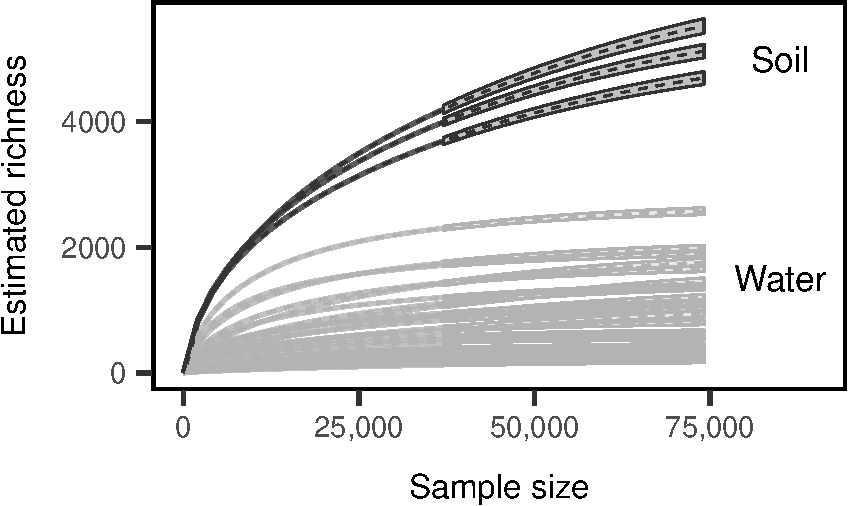
\includegraphics{ReservoirGradient_files/figure-latex/rare_extrap_plot-1} \end{center}

Next, we'll extract the estimates for the Hill numbers at different
levels of q, which differentially weight common versus rare species.

\begin{Shaded}
\begin{Highlighting}[]
\NormalTok{hill.estim <-}\StringTok{ }\NormalTok{divestim}\OperatorTok{$}\NormalTok{AsyEst }\OperatorTok\StringTok{ }\KeywordTok{filter}\NormalTok{(Diversity }\OperatorTok{==}\StringTok{ "Species richness"}\NormalTok{) }\OperatorTok\StringTok{ }
\StringTok{  }\KeywordTok{left_join}\NormalTok{(}\KeywordTok{rownames_to_column}\NormalTok{(alpha.div), }\DataTypeTok{by =} \KeywordTok{c}\NormalTok{(}\StringTok{"Observed"}\NormalTok{ =}\StringTok{ "S.obs"}\NormalTok{)) }\OperatorTok\StringTok{ }
\StringTok{  }\KeywordTok{select}\NormalTok{(Site, rowname, station, molecule, type, distance) }\OperatorTok\StringTok{ }
\StringTok{  }\KeywordTok{left_join}\NormalTok{(divestim}\OperatorTok{$}\NormalTok{AsyEst, }\DataTypeTok{by =} \StringTok{"Site"}\NormalTok{)}

\NormalTok{hill.water <-}\StringTok{ }\KeywordTok{as_tibble}\NormalTok{(hill.estim) }\OperatorTok\StringTok{ }\KeywordTok{filter}\NormalTok{(type }\OperatorTok{==}\StringTok{ "water"}\NormalTok{)}
\NormalTok{hill.water.rich <-}\StringTok{ }\KeywordTok{subset}\NormalTok{(hill.water, Diversity }\OperatorTok{==}\StringTok{ "Species richness"}\NormalTok{)}
\NormalTok{hill.water.shan <-}\StringTok{ }\KeywordTok{subset}\NormalTok{(hill.water, Diversity }\OperatorTok{==}\StringTok{ "Shannon diversity"}\NormalTok{)}
\NormalTok{hill.water.simp <-}\StringTok{ }\KeywordTok{subset}\NormalTok{(hill.water, Diversity }\OperatorTok{==}\StringTok{ "Simpson diversity"}\NormalTok{)}

\NormalTok{hill.water.mod.rich <-}\StringTok{ }\KeywordTok{lm}\NormalTok{(Estimator }\OperatorTok{~}\StringTok{ }\NormalTok{distance }\OperatorTok{*}\StringTok{ }\NormalTok{molecule, }\DataTypeTok{data =}\NormalTok{ hill.water.rich)}
\NormalTok{hill.water.mod.shan <-}\StringTok{ }\KeywordTok{lm}\NormalTok{(Estimator }\OperatorTok{~}\StringTok{ }\NormalTok{distance }\OperatorTok{*}\StringTok{ }\NormalTok{molecule, }\DataTypeTok{data =}\NormalTok{ hill.water.shan)}
\NormalTok{hill.water.mod.simp <-}\StringTok{ }\KeywordTok{lm}\NormalTok{(Estimator }\OperatorTok{~}\StringTok{ }\NormalTok{distance }\OperatorTok{*}\StringTok{ }\NormalTok{molecule, }\DataTypeTok{data =}\NormalTok{ hill.water.simp)}

\CommentTok{# summary(hill.water.mod.rich)}
\CommentTok{# summary(hill.water.mod.shan)}
\CommentTok{# summary(hill.water.mod.simp)}

\CommentTok{# tidy up the model output}
\NormalTok{hill.water.mods <-}\StringTok{ }\KeywordTok{as_tibble}\NormalTok{(}\KeywordTok{rbind.data.frame}\NormalTok{(}
  \KeywordTok{tidy}\NormalTok{(hill.water.mod.rich) }\OperatorTok\StringTok{ }\KeywordTok{add_column}\NormalTok{(}\DataTypeTok{Diversity =} \StringTok{"Richness"}\NormalTok{),}
  \KeywordTok{tidy}\NormalTok{(hill.water.mod.shan) }\OperatorTok\StringTok{ }\KeywordTok{add_column}\NormalTok{(}\DataTypeTok{Diversity =} \StringTok{"Shannon"}\NormalTok{),}
  \KeywordTok{tidy}\NormalTok{(hill.water.mod.simp) }\OperatorTok\StringTok{ }\KeywordTok{add_column}\NormalTok{(}\DataTypeTok{Diversity =} \StringTok{"Simpson"}\NormalTok{)}
\NormalTok{))}
\end{Highlighting}
\end{Shaded}

\begin{Shaded}
\begin{Highlighting}[]
\CommentTok{# Summary table of the model results. }
\NormalTok{hill.water.mods }\OperatorTok\StringTok{ }
\StringTok{  }\KeywordTok{group_by}\NormalTok{(Diversity) }\OperatorTok\StringTok{ }
\StringTok{  }\KeywordTok{rename}\NormalTok{(}\StringTok{"Term"}\NormalTok{ =}\StringTok{ }\NormalTok{term, }
         \StringTok{"Estimate"}\NormalTok{ =}\StringTok{ }\NormalTok{estimate, }
         \StringTok{"Std. Error"}\NormalTok{ =}\StringTok{ }\NormalTok{std.error, }
         \StringTok{"Statistic"}\NormalTok{ =}\StringTok{ }\NormalTok{statistic, }
         \StringTok{"p-value"}\NormalTok{ =}\StringTok{ }\NormalTok{p.value) }\OperatorTok\StringTok{ }
\StringTok{  }\KeywordTok{filter}\NormalTok{(Term }\OperatorTok{!=}\StringTok{ "(Intercept)"}\NormalTok{) }\OperatorTok\StringTok{ }
\StringTok{  }\KeywordTok{select}\NormalTok{(Diversity, }\KeywordTok{everything}\NormalTok{()) }\OperatorTok\StringTok{ }
\StringTok{  }\KeywordTok{pander}\NormalTok{(}\DataTypeTok{round =} \DecValTok{4}\NormalTok{)}
\end{Highlighting}
\end{Shaded}

\begin{longtable}[]{@{}cccccc@{}}
\toprule
\begin{minipage}[b]{0.12\columnwidth}\centering\strut
Diversity\strut
\end{minipage} & \begin{minipage}[b]{0.24\columnwidth}\centering\strut
Term\strut
\end{minipage} & \begin{minipage}[b]{0.11\columnwidth}\centering\strut
Estimate\strut
\end{minipage} & \begin{minipage}[b]{0.14\columnwidth}\centering\strut
Std. Error\strut
\end{minipage} & \begin{minipage}[b]{0.12\columnwidth}\centering\strut
Statistic\strut
\end{minipage} & \begin{minipage}[b]{0.09\columnwidth}\centering\strut
p-value\strut
\end{minipage}\tabularnewline
\midrule
\endhead
\begin{minipage}[t]{0.12\columnwidth}\centering\strut
Richness\strut
\end{minipage} & \begin{minipage}[t]{0.24\columnwidth}\centering\strut
distance\strut
\end{minipage} & \begin{minipage}[t]{0.11\columnwidth}\centering\strut
4.461\strut
\end{minipage} & \begin{minipage}[t]{0.14\columnwidth}\centering\strut
0.5005\strut
\end{minipage} & \begin{minipage}[t]{0.12\columnwidth}\centering\strut
8.912\strut
\end{minipage} & \begin{minipage}[t]{0.09\columnwidth}\centering\strut
0\strut
\end{minipage}\tabularnewline
\begin{minipage}[t]{0.12\columnwidth}\centering\strut
Richness\strut
\end{minipage} & \begin{minipage}[t]{0.24\columnwidth}\centering\strut
moleculeRNA\strut
\end{minipage} & \begin{minipage}[t]{0.11\columnwidth}\centering\strut
1.364\strut
\end{minipage} & \begin{minipage}[t]{0.14\columnwidth}\centering\strut
167.2\strut
\end{minipage} & \begin{minipage}[t]{0.12\columnwidth}\centering\strut
0.0082\strut
\end{minipage} & \begin{minipage}[t]{0.09\columnwidth}\centering\strut
0.9935\strut
\end{minipage}\tabularnewline
\begin{minipage}[t]{0.12\columnwidth}\centering\strut
Richness\strut
\end{minipage} & \begin{minipage}[t]{0.24\columnwidth}\centering\strut
distance:moleculeRNA\strut
\end{minipage} & \begin{minipage}[t]{0.11\columnwidth}\centering\strut
-4.568\strut
\end{minipage} & \begin{minipage}[t]{0.14\columnwidth}\centering\strut
0.7043\strut
\end{minipage} & \begin{minipage}[t]{0.12\columnwidth}\centering\strut
-6.486\strut
\end{minipage} & \begin{minipage}[t]{0.09\columnwidth}\centering\strut
0\strut
\end{minipage}\tabularnewline
\begin{minipage}[t]{0.12\columnwidth}\centering\strut
Shannon\strut
\end{minipage} & \begin{minipage}[t]{0.24\columnwidth}\centering\strut
distance\strut
\end{minipage} & \begin{minipage}[t]{0.11\columnwidth}\centering\strut
0.2892\strut
\end{minipage} & \begin{minipage}[t]{0.14\columnwidth}\centering\strut
0.1084\strut
\end{minipage} & \begin{minipage}[t]{0.12\columnwidth}\centering\strut
2.669\strut
\end{minipage} & \begin{minipage}[t]{0.09\columnwidth}\centering\strut
0.0122\strut
\end{minipage}\tabularnewline
\begin{minipage}[t]{0.12\columnwidth}\centering\strut
Shannon\strut
\end{minipage} & \begin{minipage}[t]{0.24\columnwidth}\centering\strut
moleculeRNA\strut
\end{minipage} & \begin{minipage}[t]{0.11\columnwidth}\centering\strut
-38.48\strut
\end{minipage} & \begin{minipage}[t]{0.14\columnwidth}\centering\strut
36.2\strut
\end{minipage} & \begin{minipage}[t]{0.12\columnwidth}\centering\strut
-1.063\strut
\end{minipage} & \begin{minipage}[t]{0.09\columnwidth}\centering\strut
0.2963\strut
\end{minipage}\tabularnewline
\begin{minipage}[t]{0.12\columnwidth}\centering\strut
Shannon\strut
\end{minipage} & \begin{minipage}[t]{0.24\columnwidth}\centering\strut
distance:moleculeRNA\strut
\end{minipage} & \begin{minipage}[t]{0.11\columnwidth}\centering\strut
-0.2798\strut
\end{minipage} & \begin{minipage}[t]{0.14\columnwidth}\centering\strut
0.1525\strut
\end{minipage} & \begin{minipage}[t]{0.12\columnwidth}\centering\strut
-1.835\strut
\end{minipage} & \begin{minipage}[t]{0.09\columnwidth}\centering\strut
0.0765\strut
\end{minipage}\tabularnewline
\begin{minipage}[t]{0.12\columnwidth}\centering\strut
Simpson\strut
\end{minipage} & \begin{minipage}[t]{0.24\columnwidth}\centering\strut
distance\strut
\end{minipage} & \begin{minipage}[t]{0.11\columnwidth}\centering\strut
0.0521\strut
\end{minipage} & \begin{minipage}[t]{0.14\columnwidth}\centering\strut
0.0322\strut
\end{minipage} & \begin{minipage}[t]{0.12\columnwidth}\centering\strut
1.62\strut
\end{minipage} & \begin{minipage}[t]{0.09\columnwidth}\centering\strut
0.1158\strut
\end{minipage}\tabularnewline
\begin{minipage}[t]{0.12\columnwidth}\centering\strut
Simpson\strut
\end{minipage} & \begin{minipage}[t]{0.24\columnwidth}\centering\strut
moleculeRNA\strut
\end{minipage} & \begin{minipage}[t]{0.11\columnwidth}\centering\strut
-23.84\strut
\end{minipage} & \begin{minipage}[t]{0.14\columnwidth}\centering\strut
10.74\strut
\end{minipage} & \begin{minipage}[t]{0.12\columnwidth}\centering\strut
-2.22\strut
\end{minipage} & \begin{minipage}[t]{0.09\columnwidth}\centering\strut
0.0341\strut
\end{minipage}\tabularnewline
\begin{minipage}[t]{0.12\columnwidth}\centering\strut
Simpson\strut
\end{minipage} & \begin{minipage}[t]{0.24\columnwidth}\centering\strut
distance:moleculeRNA\strut
\end{minipage} & \begin{minipage}[t]{0.11\columnwidth}\centering\strut
-0.0381\strut
\end{minipage} & \begin{minipage}[t]{0.14\columnwidth}\centering\strut
0.0453\strut
\end{minipage} & \begin{minipage}[t]{0.12\columnwidth}\centering\strut
-0.8415\strut
\end{minipage} & \begin{minipage}[t]{0.09\columnwidth}\centering\strut
0.4067\strut
\end{minipage}\tabularnewline
\bottomrule
\end{longtable}

\begin{Shaded}
\begin{Highlighting}[]
\CommentTok{# hill.estim %>% filter(type == "water") %>% }
\CommentTok{#   mutate(molecule = ifelse(molecule == "DNA", "Total", "Active")) %>% }
\CommentTok{#   ggplot(aes(x = distance, y = Estimator, }
\CommentTok{#              ymin = LCL, ymax = UCL,}
\CommentTok{#              color = molecule, fill = molecule, shape = molecule)) + }
\CommentTok{#   geom_point(size =3) + }
\CommentTok{#   # geom_errorbar(size = .5, aes(ymin = Estimator - s.e., ymax = Estimator + s.e.), }
\CommentTok{#   #                width = 10, alpha = 0.5) +}
\CommentTok{#   geom_smooth(method = "lm", aes(linetype = molecule)) +}
\CommentTok{#   labs(x = "Reservoir distance (m)",}
\CommentTok{#        y = "") +}
\CommentTok{#   scale_color_manual(values = my.cols) +}
\CommentTok{#   scale_fill_manual(values = my.cols) + }
\CommentTok{#   theme(legend.position = c(.88,.95), strip.placement = "outside",}
\CommentTok{#         strip.text = element_text(size = 16)) +}
\CommentTok{#   scale_x_reverse() +}
\CommentTok{#   facet_grid(Diversity ~ ., scales = "free", switch = "y") +}
\CommentTok{#   guides(fill = guide_legend(override.aes=list(fill=NA)))}
  \CommentTok{#facet_grid(Diversity ~ ., scales = "free")}

\CommentTok{# postitions for labels}
\NormalTok{xpos =}\StringTok{ }\KeywordTok{max}\NormalTok{((}\KeywordTok{na.omit}\NormalTok{(hill.estim}\OperatorTok{$}\NormalTok{distance)))}
\NormalTok{yposDNA =}\StringTok{ }\KeywordTok{predict}\NormalTok{(hill.water.mod.rich, }\DataTypeTok{newdata =} \KeywordTok{data.frame}\NormalTok{(}\DataTypeTok{distance =} \DecValTok{400}\NormalTok{, }\DataTypeTok{molecule =} \StringTok{"DNA"}\NormalTok{))}
\NormalTok{yposRNA =}\StringTok{ }\KeywordTok{predict}\NormalTok{(hill.water.mod.rich, }\DataTypeTok{newdata =} \KeywordTok{data.frame}\NormalTok{(}\DataTypeTok{distance =} \DecValTok{400}\NormalTok{, }\DataTypeTok{molecule =} \StringTok{"RNA"}\NormalTok{))}
\NormalTok{alpha.fig <-}\StringTok{ }\NormalTok{hill.estim }\OperatorTok\StringTok{ }\KeywordTok{filter}\NormalTok{(type }\OperatorTok{==}\StringTok{ "water"}\NormalTok{, Diversity }\OperatorTok{==}\StringTok{ "Species richness"}\NormalTok{) }\OperatorTok\StringTok{ }
\StringTok{  }\KeywordTok{mutate}\NormalTok{(}\DataTypeTok{molecule =} \KeywordTok{ifelse}\NormalTok{(molecule }\OperatorTok{==}\StringTok{ "DNA"}\NormalTok{, }\StringTok{"Total"}\NormalTok{, }\StringTok{"Active"}\NormalTok{)) }\OperatorTok\StringTok{ }
\StringTok{  }\KeywordTok{ggplot}\NormalTok{(}\KeywordTok{aes}\NormalTok{(}\DataTypeTok{x =}\NormalTok{ distance, }\DataTypeTok{y =}\NormalTok{ Estimator, }
             \DataTypeTok{ymin =}\NormalTok{ LCL, }\DataTypeTok{ymax =}\NormalTok{ UCL,}
             \DataTypeTok{color =}\NormalTok{ molecule, }\DataTypeTok{fill =}\NormalTok{ molecule, }\DataTypeTok{shape =}\NormalTok{ molecule)) }\OperatorTok{+}\StringTok{ }
\StringTok{  }\KeywordTok{geom_point}\NormalTok{(}\DataTypeTok{size =}\DecValTok{3}\NormalTok{, }\DataTypeTok{alpha =} \FloatTok{0.8}\NormalTok{) }\OperatorTok{+}\StringTok{ }
\StringTok{  }\CommentTok{# geom_errorbar(size = .5, aes(ymin = Estimator - s.e., ymax = Estimator + s.e.), }
\StringTok{  }\CommentTok{#                width = 10, alpha = 0.5) +}
\StringTok{  }\KeywordTok{geom_smooth}\NormalTok{(}\DataTypeTok{method =} \StringTok{"lm"}\NormalTok{, }\KeywordTok{aes}\NormalTok{(}\DataTypeTok{linetype =}\NormalTok{ molecule)) }\OperatorTok{+}
\StringTok{  }\KeywordTok{labs}\NormalTok{(}\DataTypeTok{x =} \StringTok{"Reservoir distance (m)"}\NormalTok{,}
       \DataTypeTok{y =} \StringTok{"Estimated richness"}\NormalTok{) }\OperatorTok{+}
\StringTok{  }\KeywordTok{scale_x_reverse}\NormalTok{(}\DataTypeTok{limits =} \KeywordTok{c}\NormalTok{(}\DecValTok{400}\NormalTok{,}\DecValTok{0}\NormalTok{)) }\OperatorTok{+}
\StringTok{  }\KeywordTok{scale_y_continuous}\NormalTok{(}\DataTypeTok{breaks =} \KeywordTok{seq}\NormalTok{(}\DecValTok{0}\NormalTok{, }\DecValTok{3000}\NormalTok{, }\DataTypeTok{by =} \DecValTok{500}\NormalTok{)) }\OperatorTok{+}
\StringTok{  }\KeywordTok{scale_color_manual}\NormalTok{(}\DataTypeTok{values =}\NormalTok{ my.cols) }\OperatorTok{+}
\StringTok{  }\KeywordTok{scale_fill_manual}\NormalTok{(}\DataTypeTok{values =}\NormalTok{ my.cols) }\OperatorTok{+}
\StringTok{  }\KeywordTok{theme}\NormalTok{(}\DataTypeTok{legend.position =} \StringTok{"none"}\NormalTok{) }\OperatorTok{+}
\StringTok{  }\KeywordTok{guides}\NormalTok{(}\DataTypeTok{fill =} \KeywordTok{guide_legend}\NormalTok{(}\DataTypeTok{override.aes=}\KeywordTok{list}\NormalTok{(}\DataTypeTok{fill=}\OtherTok{NA}\NormalTok{))) }\OperatorTok{+}
\StringTok{  }\KeywordTok{annotate}\NormalTok{(}\StringTok{"text"}\NormalTok{, }\DataTypeTok{x =} \DecValTok{375}\NormalTok{, }\DataTypeTok{y =}\NormalTok{ yposRNA }\OperatorTok{+}\StringTok{ }\DecValTok{300}\NormalTok{, }
           \DataTypeTok{label =} \StringTok{"Active"}\NormalTok{, }\DataTypeTok{size =} \DecValTok{5}\NormalTok{) }\OperatorTok{+}
\StringTok{  }\KeywordTok{annotate}\NormalTok{(}\StringTok{"text"}\NormalTok{, }\DataTypeTok{x =} \DecValTok{375}\NormalTok{, }\DataTypeTok{y =}\NormalTok{ yposDNA }\OperatorTok{+}\StringTok{ }\DecValTok{300}\NormalTok{, }
           \DataTypeTok{label =} \StringTok{"Total"}\NormalTok{, }\DataTypeTok{size =} \DecValTok{5}\NormalTok{) }\OperatorTok{+}
\StringTok{  }\KeywordTok{annotate}\NormalTok{(}\DataTypeTok{geom =} \StringTok{"text"}\NormalTok{, }\DataTypeTok{x =} \DecValTok{0}\NormalTok{, }\DataTypeTok{y =} \DecValTok{2750}\NormalTok{, }\DataTypeTok{hjust =} \DecValTok{1}\NormalTok{, }\DataTypeTok{vjust =} \DecValTok{1}\NormalTok{, }\DataTypeTok{size =} \DecValTok{5}\NormalTok{,}
           \DataTypeTok{label =} \KeywordTok{paste0}\NormalTok{(}\StringTok{"r^2== "}\NormalTok{,}\KeywordTok{round}\NormalTok{(}\KeywordTok{summary}\NormalTok{(hill.water.mod.rich)}\OperatorTok{$}\NormalTok{r.squared, }\DecValTok{2}\NormalTok{)), }\DataTypeTok{parse =}\NormalTok{ T) }\OperatorTok{+}
\StringTok{  }\KeywordTok{ggsave}\NormalTok{(}\StringTok{"figures/alpha_fig.pdf"}\NormalTok{)}
\NormalTok{alpha.fig}
\end{Highlighting}
\end{Shaded}

\begin{center}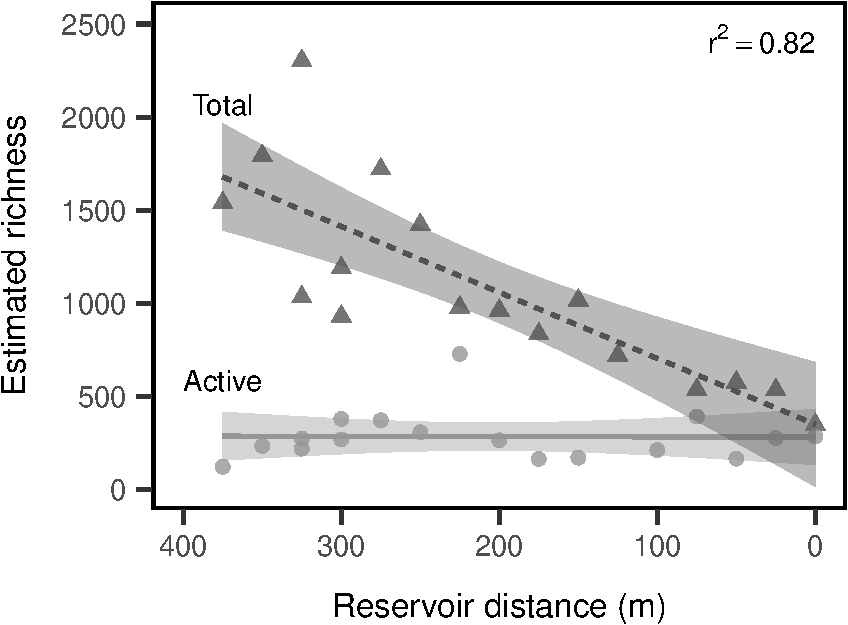
\includegraphics{ReservoirGradient_files/figure-latex/hill_div_plot-1} \end{center}

So, from the basis of these results, we can make the following
conclusions. First, we note that diversity in the total community decays
from the stream inlet to the dam of the reservoir. That is, all the
lines have a negative slope. However, we do not see this decay in the
metabolically active community. Second, we note that the metabolically
actively community has much lower diversity than the total community
near the soils, but this difference decreases toward the dam. Last,
because we quantified diversity across three orders of Hill numbers (q =
0, 1, and 2), we can also say something about the relative importance of
rare versus common taxa along the reservoir transect. We see the the
significance of the distance-by-molecule interaction term decrease as
rare taxa are downweighted in favor of common taxa. This suggests that
the differences between the active and total communities along the
transect is driven primarily by rare taxa. However, the general trend of
higher Simpson diversity across the whole transect suggests that
low-activity, but relatively common, taxa are maintained in the
reservoir.

\subsection{Similarity To Terrestrial Habitat Across Gradient
(Terrestrial
Influence)}\label{similarity-to-terrestrial-habitat-across-gradient-terrestrial-influence}

Here, we fit a linear model to the similarity of the aquatic community
to the soil community.

\begin{Shaded}
\begin{Highlighting}[]
\CommentTok{# Similarity to Soil Sample}
\NormalTok{UL.bray      <-}\StringTok{ }\DecValTok{1}\OperatorTok{-}\KeywordTok{as.matrix}\NormalTok{(}\KeywordTok{vegdist}\NormalTok{(OTUsREL.log, }\DataTypeTok{method=}\StringTok{"bray"}\NormalTok{))}
\NormalTok{UL.bray.lake <-}\StringTok{ }\NormalTok{UL.bray[}\OperatorTok{-}\KeywordTok{c}\NormalTok{(}\DecValTok{1}\OperatorTok{:}\DecValTok{3}\NormalTok{), }\DecValTok{1}\OperatorTok{:}\DecValTok{3}\NormalTok{] }
\NormalTok{bray.mean    <-}\StringTok{ }\KeywordTok{round}\NormalTok{(}\KeywordTok{apply}\NormalTok{(UL.bray.lake, }\DecValTok{1}\NormalTok{, mean), }\DecValTok{3}\NormalTok{)}
\NormalTok{bray.se      <-}\StringTok{ }\KeywordTok{round}\NormalTok{(}\KeywordTok{apply}\NormalTok{(UL.bray.lake, }\DecValTok{1}\NormalTok{, se), }\DecValTok{3}\NormalTok{)}
\NormalTok{UL.sim       <-}\StringTok{ }\KeywordTok{cbind}\NormalTok{(design[}\OperatorTok{-}\KeywordTok{c}\NormalTok{(}\DecValTok{1}\OperatorTok{:}\DecValTok{3}\NormalTok{), ], bray.mean, bray.se)}

\CommentTok{# Calculate Linear Model}
\NormalTok{model.terr <-}\StringTok{ }\KeywordTok{lm}\NormalTok{(bray.mean }\OperatorTok{~}\StringTok{ }\NormalTok{distance }\OperatorTok{*}\StringTok{ }\NormalTok{molecule, }\DataTypeTok{data =}\NormalTok{ UL.sim)}
\KeywordTok{pander}\NormalTok{(model.terr)}
\end{Highlighting}
\end{Shaded}

\begin{longtable}[]{@{}ccccc@{}}
\caption{Fitting linear model: bray.mean \textasciitilde{} distance *
molecule}\tabularnewline
\toprule
\begin{minipage}[b]{0.31\columnwidth}\centering\strut
~\strut
\end{minipage} & \begin{minipage}[b]{0.15\columnwidth}\centering\strut
Estimate\strut
\end{minipage} & \begin{minipage}[b]{0.15\columnwidth}\centering\strut
Std. Error\strut
\end{minipage} & \begin{minipage}[b]{0.13\columnwidth}\centering\strut
t value\strut
\end{minipage} & \begin{minipage}[b]{0.13\columnwidth}\centering\strut
Pr(\textgreater{}\textbar{}t\textbar{})\strut
\end{minipage}\tabularnewline
\midrule
\endfirsthead
\toprule
\begin{minipage}[b]{0.31\columnwidth}\centering\strut
~\strut
\end{minipage} & \begin{minipage}[b]{0.15\columnwidth}\centering\strut
Estimate\strut
\end{minipage} & \begin{minipage}[b]{0.15\columnwidth}\centering\strut
Std. Error\strut
\end{minipage} & \begin{minipage}[b]{0.13\columnwidth}\centering\strut
t value\strut
\end{minipage} & \begin{minipage}[b]{0.13\columnwidth}\centering\strut
Pr(\textgreater{}\textbar{}t\textbar{})\strut
\end{minipage}\tabularnewline
\midrule
\endhead
\begin{minipage}[t]{0.31\columnwidth}\centering\strut
\textbf{(Intercept)}\strut
\end{minipage} & \begin{minipage}[t]{0.15\columnwidth}\centering\strut
0.02739\strut
\end{minipage} & \begin{minipage}[t]{0.15\columnwidth}\centering\strut
0.01774\strut
\end{minipage} & \begin{minipage}[t]{0.13\columnwidth}\centering\strut
1.544\strut
\end{minipage} & \begin{minipage}[t]{0.13\columnwidth}\centering\strut
0.1331\strut
\end{minipage}\tabularnewline
\begin{minipage}[t]{0.31\columnwidth}\centering\strut
\textbf{distance}\strut
\end{minipage} & \begin{minipage}[t]{0.15\columnwidth}\centering\strut
0.0004004\strut
\end{minipage} & \begin{minipage}[t]{0.15\columnwidth}\centering\strut
7.464e-05\strut
\end{minipage} & \begin{minipage}[t]{0.13\columnwidth}\centering\strut
5.365\strut
\end{minipage} & \begin{minipage}[t]{0.13\columnwidth}\centering\strut
8.319e-06\strut
\end{minipage}\tabularnewline
\begin{minipage}[t]{0.31\columnwidth}\centering\strut
\textbf{moleculeRNA}\strut
\end{minipage} & \begin{minipage}[t]{0.15\columnwidth}\centering\strut
-0.0003186\strut
\end{minipage} & \begin{minipage}[t]{0.15\columnwidth}\centering\strut
0.02493\strut
\end{minipage} & \begin{minipage}[t]{0.13\columnwidth}\centering\strut
-0.01278\strut
\end{minipage} & \begin{minipage}[t]{0.13\columnwidth}\centering\strut
0.9899\strut
\end{minipage}\tabularnewline
\begin{minipage}[t]{0.31\columnwidth}\centering\strut
\textbf{distance:moleculeRNA}\strut
\end{minipage} & \begin{minipage}[t]{0.15\columnwidth}\centering\strut
-0.0003913\strut
\end{minipage} & \begin{minipage}[t]{0.15\columnwidth}\centering\strut
0.000105\strut
\end{minipage} & \begin{minipage}[t]{0.13\columnwidth}\centering\strut
-3.726\strut
\end{minipage} & \begin{minipage}[t]{0.13\columnwidth}\centering\strut
0.000806\strut
\end{minipage}\tabularnewline
\bottomrule
\end{longtable}

\begin{Shaded}
\begin{Highlighting}[]
\CommentTok{# # Calculate Confidance Intervals of Model}
\CommentTok{# newdata.terr <- data.frame(cbind(UL.sim$molecule, UL.sim$distance))}
\CommentTok{# conf95.terr <- predict(model.terr, newdata.terr, interval="confidence")}
\CommentTok{# }
\CommentTok{# # Dummy Variables Regression Model ("Terrestrial Influence")}
\CommentTok{# D2 <- (UL.sim$molecule == "RNA")*1}
\CommentTok{# fit.Fig.3b <- lm(UL.sim$bray.mean ~ UL.sim$distance + D2 + UL.sim$distance*D2)}
\CommentTok{# D2.R2 <- round(summary(fit.Fig.3b)$r.squared, 2)}
\CommentTok{# summary(fit.Fig.3b)}
\CommentTok{# }
\CommentTok{# }
\CommentTok{# DNA.int.3b <- fit.Fig.3b$coefficients[1]}
\CommentTok{# DNA.slp.3b <- fit.Fig.3b$coefficients[2]}
\CommentTok{# RNA.int.3b <- DNA.int.3b + fit.Fig.3b$coefficients[3]}
\CommentTok{# RNA.slp.3b <- DNA.slp.3b + fit.Fig.3b$coefficients[4]}
\end{Highlighting}
\end{Shaded}

\begin{Shaded}
\begin{Highlighting}[]
\NormalTok{similarity.plot <-}\StringTok{ }\NormalTok{UL.sim }\OperatorTok\StringTok{ }
\StringTok{  }\KeywordTok{mutate}\NormalTok{(}\DataTypeTok{molecule =} \KeywordTok{ifelse}\NormalTok{(UL.sim}\OperatorTok{$}\NormalTok{molecule }\OperatorTok{==}\StringTok{ "DNA"}\NormalTok{, }\StringTok{"Total"}\NormalTok{, }\StringTok{"Active"}\NormalTok{)) }\OperatorTok\StringTok{ }
\StringTok{  }\KeywordTok{ggplot}\NormalTok{(}\KeywordTok{aes}\NormalTok{(}\DataTypeTok{x =}\NormalTok{ distance, }\DataTypeTok{y =}\NormalTok{ bray.mean, }
             \DataTypeTok{color =}\NormalTok{ molecule, }\DataTypeTok{fill =}\NormalTok{ molecule, }\DataTypeTok{shape =}\NormalTok{ molecule)) }\OperatorTok{+}
\StringTok{  }\KeywordTok{geom_point}\NormalTok{(}\DataTypeTok{alpha =} \FloatTok{0.8}\NormalTok{, }\DataTypeTok{size =} \DecValTok{3}\NormalTok{, }\DataTypeTok{show.legend =}\NormalTok{ T) }\OperatorTok{+}\StringTok{ }
\StringTok{  }\KeywordTok{geom_smooth}\NormalTok{(}\DataTypeTok{method =} \StringTok{"lm"}\NormalTok{, }\DataTypeTok{show.legend =}\NormalTok{ T, }\KeywordTok{aes}\NormalTok{(}\DataTypeTok{linetype =}\NormalTok{ molecule)) }\OperatorTok{+}\StringTok{ }
\StringTok{  }\KeywordTok{labs}\NormalTok{(}\DataTypeTok{y =} \KeywordTok{str_wrap}\NormalTok{(}\StringTok{"Percent similarity to soil community"}\NormalTok{, }\DataTypeTok{width =} \DecValTok{20}\NormalTok{), }
       \DataTypeTok{x =} \StringTok{"Reservoir distance (m)"}\NormalTok{) }\OperatorTok{+}\StringTok{ }
\StringTok{  }\KeywordTok{scale_color_manual}\NormalTok{(}\DataTypeTok{values =}\NormalTok{ my.cols) }\OperatorTok{+}\StringTok{ }
\StringTok{  }\KeywordTok{scale_fill_manual}\NormalTok{(}\DataTypeTok{values =}\NormalTok{ my.cols) }\OperatorTok{+}
\StringTok{  }\KeywordTok{theme}\NormalTok{(}\DataTypeTok{legend.position =} \StringTok{"none"}\NormalTok{) }\OperatorTok{+}
\StringTok{  }\KeywordTok{scale_x_reverse}\NormalTok{(}\DataTypeTok{limits =} \KeywordTok{c}\NormalTok{(}\DecValTok{400}\NormalTok{,}\DecValTok{0}\NormalTok{)) }\OperatorTok{+}\StringTok{ }
\StringTok{  }\KeywordTok{annotate}\NormalTok{(}\DataTypeTok{geom =} \StringTok{"text"}\NormalTok{, }\DataTypeTok{x =} \DecValTok{0}\NormalTok{, }\DataTypeTok{y =} \KeywordTok{max}\NormalTok{(UL.sim}\OperatorTok{$}\NormalTok{bray.mean), }\DataTypeTok{hjust =} \DecValTok{1}\NormalTok{, }\DataTypeTok{vjust =} \DecValTok{1}\NormalTok{, }\DataTypeTok{size =} \DecValTok{5}\NormalTok{,}
           \DataTypeTok{label =} \KeywordTok{paste0}\NormalTok{(}\StringTok{"r^2== "}\NormalTok{,}\KeywordTok{round}\NormalTok{(}\KeywordTok{summary}\NormalTok{(model.terr)}\OperatorTok{$}\NormalTok{r.squared, }\DecValTok{2}\NormalTok{)), }\DataTypeTok{parse =}\NormalTok{ T) }\OperatorTok{+}
\StringTok{  }\KeywordTok{annotate}\NormalTok{(}\StringTok{"text"}\NormalTok{, }\DataTypeTok{x =} \DecValTok{375}\NormalTok{, }\DataTypeTok{y =}\NormalTok{ .}\DecValTok{065}\NormalTok{, }\DataTypeTok{label =} \StringTok{"Active"}\NormalTok{, }\DataTypeTok{size =} \DecValTok{5}\NormalTok{) }\OperatorTok{+}
\StringTok{  }\KeywordTok{annotate}\NormalTok{(}\StringTok{"text"}\NormalTok{, }\DataTypeTok{x =} \DecValTok{375}\NormalTok{, }\DataTypeTok{y =}\NormalTok{ .}\DecValTok{24}\NormalTok{, }\DataTypeTok{label =} \StringTok{"Total"}\NormalTok{, }\DataTypeTok{size =} \DecValTok{5}\NormalTok{) }\OperatorTok{+}
\StringTok{  }\KeywordTok{ggsave}\NormalTok{(}\StringTok{"figures/similarity_fig.pdf"}\NormalTok{)}

\NormalTok{similarity.plot}
\end{Highlighting}
\end{Shaded}

\begin{center}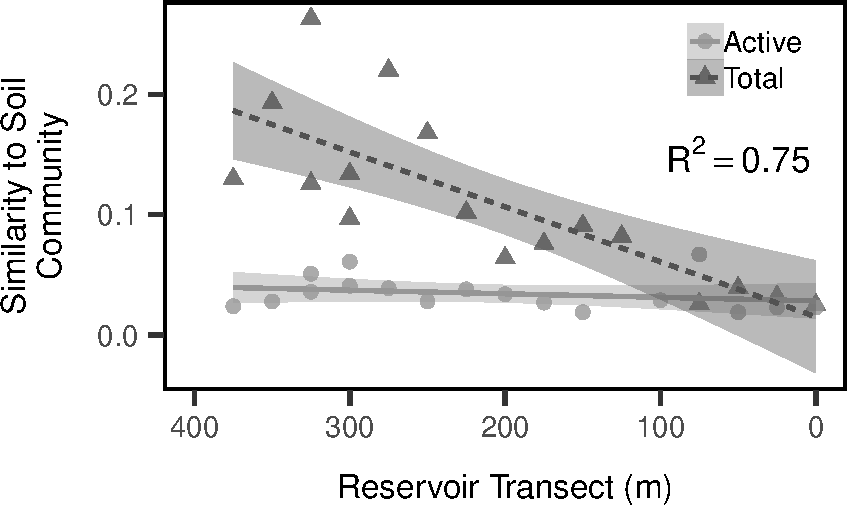
\includegraphics{ReservoirGradient_files/figure-latex/plot_similarity_to_soils-1} \end{center}

We find that our model captures most of the variation in community
structure \((R^2 = 0.7084136)\). We note a significant influence of
distance on community similarity and the presence of a significant
interaction between distance and whether the comparison is for active or
total bacterial communities. This indicates that total communities decay
faster with distance to soils than active communities do, which might be
explained by the large difference in initial intercept. Active
communities are always highly dissimilar to soil communities and remain
so across the lake, while total lake communities are initially similar
to soils, but this influence dissipates with distance into the
reservoir.

\subsubsection{Create combined figure}\label{create-combined-figure}

\begin{Shaded}
\begin{Highlighting}[]
\KeywordTok{plot_grid}\NormalTok{(alpha.fig }\OperatorTok{+}\StringTok{ }\KeywordTok{labs}\NormalTok{(}\DataTypeTok{x =} \StringTok{""}\NormalTok{), similarity.plot, }
          \DataTypeTok{align =} \StringTok{"hv"}\NormalTok{,}
          \DataTypeTok{labels =} \StringTok{"auto"}\NormalTok{, }\DataTypeTok{ncol =} \DecValTok{1}\NormalTok{) }\OperatorTok{+}
\StringTok{  }\KeywordTok{ggsave}\NormalTok{(}\StringTok{"figures/alpha_similarity_paneled.pdf"}\NormalTok{)}
\end{Highlighting}
\end{Shaded}

\begin{center}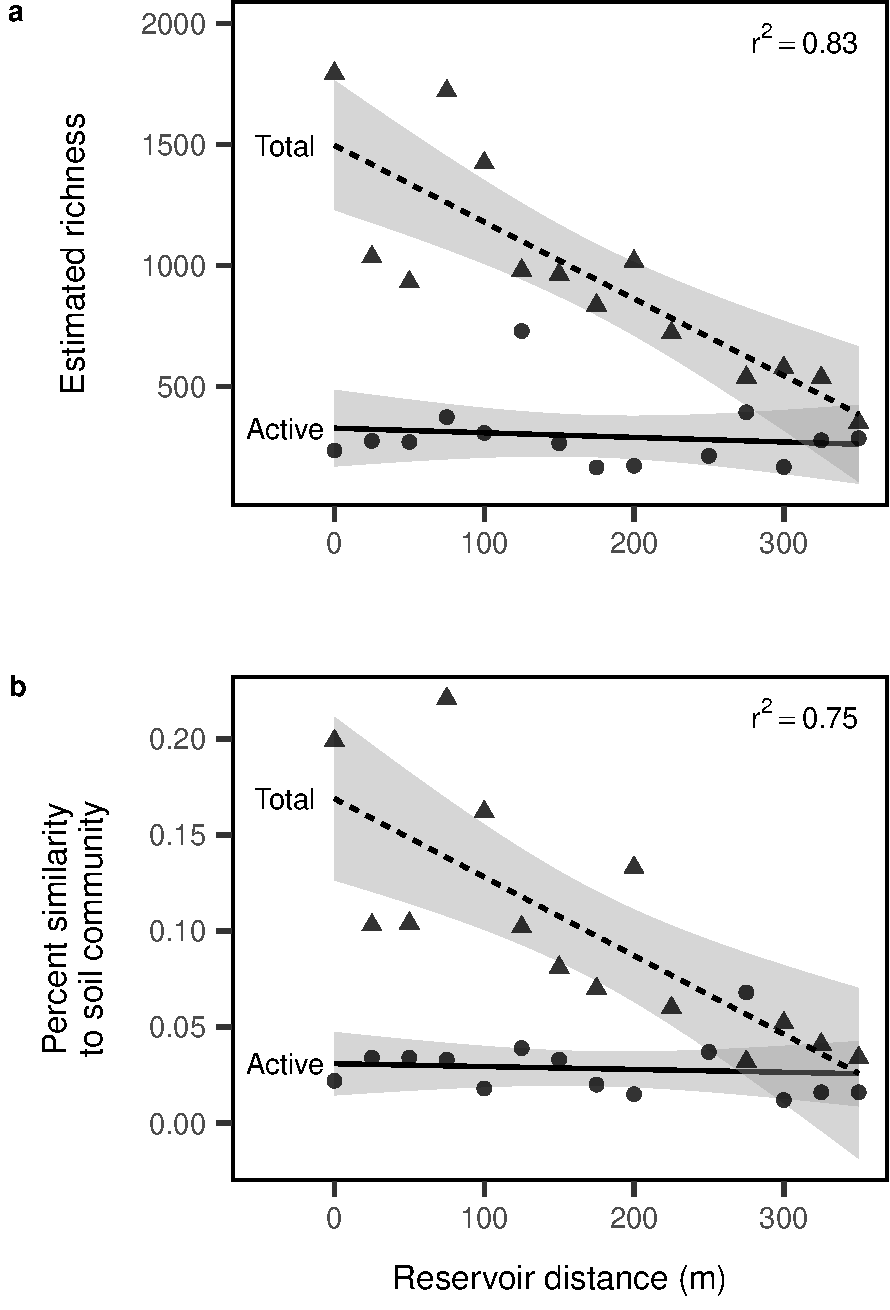
\includegraphics{ReservoirGradient_files/figure-latex/combined-plots-1} \end{center}

\subsection{How does community structure change along the
gradient?}\label{how-does-community-structure-change-along-the-gradient}

First, we'll just get an overview of how the communities look along the
aquatic transect.

\begin{Shaded}
\begin{Highlighting}[]
\NormalTok{ul.pcoa <-}\StringTok{ }\KeywordTok{cmdscale}\NormalTok{(}\KeywordTok{vegdist}\NormalTok{(OTUsREL.log, }\DataTypeTok{method=}\StringTok{"bray"}\NormalTok{), }\DecValTok{2}\NormalTok{, }\DataTypeTok{eig =}\NormalTok{ T, }\DataTypeTok{add =}\NormalTok{ T)}
\NormalTok{explainvars <-}\StringTok{ }\KeywordTok{round}\NormalTok{(}\KeywordTok{eigenvals}\NormalTok{(ul.pcoa)[}\KeywordTok{c}\NormalTok{(}\DecValTok{1}\NormalTok{,}\DecValTok{2}\NormalTok{)]}\OperatorTok{/}\KeywordTok{sum}\NormalTok{(}\KeywordTok{eigenvals}\NormalTok{(ul.pcoa)),}\DecValTok{3}\NormalTok{) }\OperatorTok{*}\DecValTok{100}
\NormalTok{water.pcvals <-}\StringTok{ }\KeywordTok{data.frame}\NormalTok{(}\KeywordTok{scores}\NormalTok{(ul.pcoa)) }\OperatorTok\StringTok{ }
\StringTok{  }\KeywordTok{rownames_to_column}\NormalTok{(}\StringTok{"name"}\NormalTok{) }\OperatorTok\StringTok{ }
\StringTok{  }\KeywordTok{left_join}\NormalTok{(}\KeywordTok{rownames_to_column}\NormalTok{(design, }\StringTok{"name"}\NormalTok{)) }\OperatorTok\StringTok{ }
\StringTok{  }\KeywordTok{arrange}\NormalTok{(}\KeywordTok{desc}\NormalTok{(distance)) }\OperatorTok\StringTok{ }\KeywordTok{filter}\NormalTok{(type }\OperatorTok{==}\StringTok{ "water"}\NormalTok{)}
\NormalTok{soil.pcvals <-}\StringTok{ }\KeywordTok{data.frame}\NormalTok{(}\KeywordTok{scores}\NormalTok{(ul.pcoa)) }\OperatorTok\StringTok{ }
\StringTok{  }\KeywordTok{rownames_to_column}\NormalTok{(}\StringTok{"name"}\NormalTok{) }\OperatorTok\StringTok{ }
\StringTok{  }\KeywordTok{left_join}\NormalTok{(}\KeywordTok{rownames_to_column}\NormalTok{(design, }\StringTok{"name"}\NormalTok{)) }\OperatorTok\StringTok{ }
\StringTok{  }\KeywordTok{arrange}\NormalTok{(}\KeywordTok{desc}\NormalTok{(distance)) }\OperatorTok\StringTok{ }\KeywordTok{filter}\NormalTok{(type }\OperatorTok{==}\StringTok{ "soil"}\NormalTok{)}
\NormalTok{pc_dists <-}\StringTok{ }\KeywordTok{tibble}\NormalTok{(}
  \DataTypeTok{DNA_dim1 =} \KeywordTok{subset}\NormalTok{(water.pcvals, molecule }\OperatorTok{==}\StringTok{ "DNA"}\NormalTok{)}\OperatorTok{$}\NormalTok{Dim1,}
  \DataTypeTok{DNA_dim2 =} \KeywordTok{subset}\NormalTok{(water.pcvals, molecule }\OperatorTok{==}\StringTok{ "DNA"}\NormalTok{)}\OperatorTok{$}\NormalTok{Dim2,}
  \DataTypeTok{RNA_dim1 =} \KeywordTok{subset}\NormalTok{(water.pcvals, molecule }\OperatorTok{==}\StringTok{ "RNA"}\NormalTok{)}\OperatorTok{$}\NormalTok{Dim1,}
  \DataTypeTok{RNA_dim2 =} \KeywordTok{subset}\NormalTok{(water.pcvals, molecule }\OperatorTok{==}\StringTok{ "RNA"}\NormalTok{)}\OperatorTok{$}\NormalTok{Dim2)}
\NormalTok{pcoa.fig <-}\StringTok{ }\KeywordTok{data.frame}\NormalTok{(}\KeywordTok{scores}\NormalTok{(ul.pcoa)) }\OperatorTok\StringTok{ }
\StringTok{  }\KeywordTok{rownames_to_column}\NormalTok{(}\StringTok{"name"}\NormalTok{) }\OperatorTok\StringTok{ }
\StringTok{  }\KeywordTok{left_join}\NormalTok{(}\KeywordTok{rownames_to_column}\NormalTok{(design, }\StringTok{"name"}\NormalTok{)) }\OperatorTok\StringTok{ }
\StringTok{  }\KeywordTok{arrange}\NormalTok{(}\KeywordTok{desc}\NormalTok{(distance)) }\OperatorTok\StringTok{ }\KeywordTok{filter}\NormalTok{(type }\OperatorTok{==}\StringTok{ "water"}\NormalTok{) }\OperatorTok\StringTok{ }
\StringTok{  }\KeywordTok{mutate}\NormalTok{(}\DataTypeTok{molecule =} \KeywordTok{ifelse}\NormalTok{(molecule }\OperatorTok{==}\StringTok{ "DNA"}\NormalTok{, }\StringTok{"Total"}\NormalTok{, }\StringTok{"Active"}\NormalTok{)) }\OperatorTok\StringTok{ }
\StringTok{  }\KeywordTok{ggplot}\NormalTok{(}\KeywordTok{aes}\NormalTok{(}\DataTypeTok{x =}\NormalTok{ Dim1, }\DataTypeTok{y =}\NormalTok{ Dim2)) }\OperatorTok{+}
\StringTok{  }\KeywordTok{geom_path}\NormalTok{(}\DataTypeTok{size =} \DecValTok{1}\NormalTok{, }\DataTypeTok{alpha =} \FloatTok{0.75}\NormalTok{, }\DataTypeTok{arrow =} \KeywordTok{arrow}\NormalTok{(}\DataTypeTok{angle =} \DecValTok{20}\NormalTok{,}
                          \DataTypeTok{length =} \KeywordTok{unit}\NormalTok{(}\FloatTok{0.35}\NormalTok{, }\StringTok{"cm"}\NormalTok{),}
                          \DataTypeTok{type =} \StringTok{"closed"}\NormalTok{), }\KeywordTok{aes}\NormalTok{(}\DataTypeTok{color =}\NormalTok{ molecule, }\DataTypeTok{linetype =}\NormalTok{ molecule)) }\OperatorTok{+}
\StringTok{  }\KeywordTok{geom_point}\NormalTok{(}\DataTypeTok{size =} \DecValTok{3}\NormalTok{, }\DataTypeTok{alpha =} \FloatTok{0.8}\NormalTok{, }\KeywordTok{aes}\NormalTok{(}\DataTypeTok{color =}\NormalTok{ molecule, }\DataTypeTok{shape =}\NormalTok{ molecule)) }\OperatorTok{+}\StringTok{ }
\StringTok{  }\KeywordTok{geom_point}\NormalTok{(}\DataTypeTok{data =} \KeywordTok{select}\NormalTok{(soil.pcvals, Dim1, Dim2), }\DataTypeTok{col =} \StringTok{"black"}\NormalTok{, }\DataTypeTok{alpha =}\NormalTok{ .}\DecValTok{8}\NormalTok{, }\DataTypeTok{size =} \DecValTok{3}\NormalTok{) }\OperatorTok{+}
\StringTok{  }\KeywordTok{scale_color_manual}\NormalTok{(}\StringTok{"Community Subset"}\NormalTok{, }\DataTypeTok{values =}\NormalTok{ my.cols) }\OperatorTok{+}
\StringTok{  }\KeywordTok{geom_segment}\NormalTok{(}\DataTypeTok{data =}\NormalTok{ pc_dists,}
               \KeywordTok{aes}\NormalTok{(}\DataTypeTok{x =}\NormalTok{ DNA_dim1, }\DataTypeTok{y =}\NormalTok{ DNA_dim2,}
                   \DataTypeTok{xend =}\NormalTok{ RNA_dim1, }\DataTypeTok{yend =}\NormalTok{ RNA_dim2),}
               \DataTypeTok{alpha =} \DecValTok{0}\NormalTok{) }\OperatorTok{+}
\StringTok{  }\CommentTok{#coord_fixed(ratio = 1, xlim = c(-.4, .4)) +}
\StringTok{  }\KeywordTok{labs}\NormalTok{(}\DataTypeTok{x =} \KeywordTok{paste0}\NormalTok{(}\StringTok{"PCoA 1 ("}\NormalTok{, explainvars[}\DecValTok{1}\NormalTok{],}\StringTok{"%)"}\NormalTok{),}
       \DataTypeTok{y =} \KeywordTok{paste0}\NormalTok{(}\StringTok{"PCoA 2 ("}\NormalTok{, explainvars[}\DecValTok{2}\NormalTok{],}\StringTok{"%)"}\NormalTok{)) }\OperatorTok{+}
\StringTok{  }\KeywordTok{theme}\NormalTok{(}\DataTypeTok{legend.position =} \StringTok{"none"}\NormalTok{) }\OperatorTok{+}
\StringTok{  }\KeywordTok{annotate}\NormalTok{(}\DataTypeTok{geom =} \StringTok{"text"}\NormalTok{, }\DataTypeTok{x =}\NormalTok{ .}\DecValTok{2}\NormalTok{, }\DataTypeTok{y =} \DecValTok{0}\NormalTok{, }\DataTypeTok{label =} \StringTok{"Active"}\NormalTok{, }\DataTypeTok{size =} \DecValTok{5}\NormalTok{) }\OperatorTok{+}
\StringTok{  }\KeywordTok{annotate}\NormalTok{(}\DataTypeTok{geom =} \StringTok{"text"}\NormalTok{, }\DataTypeTok{x =} \OperatorTok{-}\NormalTok{.}\DecValTok{25}\NormalTok{, }\DataTypeTok{y =} \OperatorTok{-}\NormalTok{.}\DecValTok{3}\NormalTok{, }\DataTypeTok{label =} \StringTok{"Total"}\NormalTok{, }\DataTypeTok{size =} \DecValTok{5}\NormalTok{) }\OperatorTok{+}\StringTok{ }
\StringTok{  }\KeywordTok{annotate}\NormalTok{(}\DataTypeTok{geom =} \StringTok{"text"}\NormalTok{, }\DataTypeTok{x =}\NormalTok{ .}\DecValTok{3}\NormalTok{, }\DataTypeTok{y =} \OperatorTok{-}\NormalTok{.}\DecValTok{4}\NormalTok{, }\DataTypeTok{label =} \StringTok{"Soils"}\NormalTok{, }\DataTypeTok{size =} \DecValTok{5}\NormalTok{) }\OperatorTok{+}
\StringTok{  }\KeywordTok{ggsave}\NormalTok{(}\StringTok{"figures/pcoa.pdf"}\NormalTok{)}
\NormalTok{pcoa.fig}
\end{Highlighting}
\end{Shaded}

\begin{center}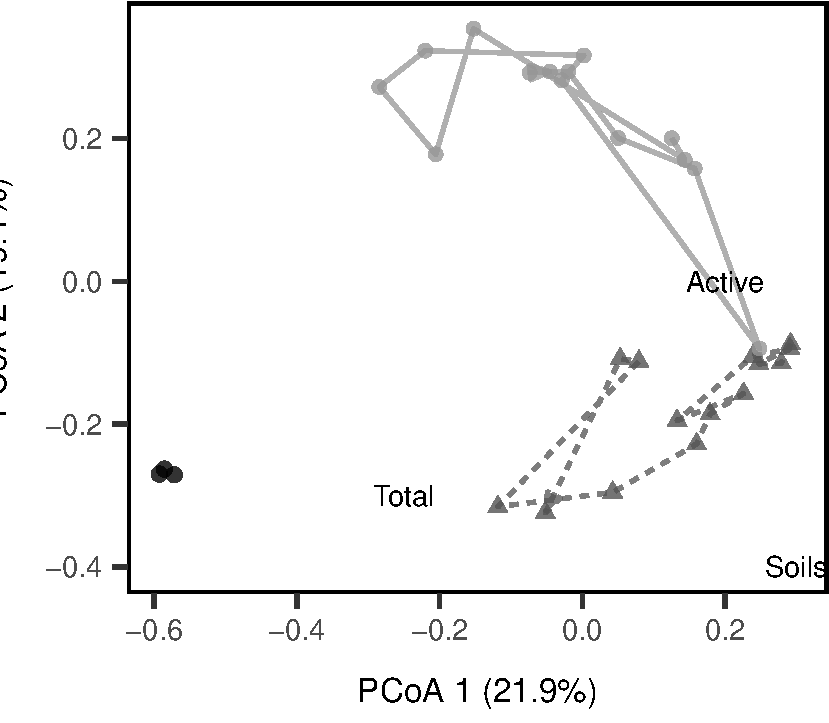
\includegraphics{ReservoirGradient_files/figure-latex/ordination-1} \end{center}

So, it appears that there is convergence in community structure along
the path from stream inlet to the dam. This could reflect a loss of
soil-derived taxa in the aquatic samples. To test this, we'll look at
\(\beta\)-diversity along the gradient with respect to the soil samples.
If we see a decay in similarity to soils, this suggests soil taxa are
having a comparatively lower influence with distance from the inlet.

\section{Identifying the Soil
Bacteria}\label{identifying-the-soil-bacteria}

Now, we wish to determine whether soil-derived taxa are driving this
pattern, and then ask who these influential soil bacteria are.

To classify soil bacteria, we take an incidence-based approach and
classify OTUs as:\\
- present in the soil and present, but never active, in the reservoir\\
- present in the soil and active in the reservoir

\begin{Shaded}
\begin{Highlighting}[]
\CommentTok{# separate lake and soil samples}
\NormalTok{lake.total <-}\StringTok{ }\NormalTok{OTUs[}\KeywordTok{which}\NormalTok{(design}\OperatorTok{$}\NormalTok{molecule }\OperatorTok{==}\StringTok{ "DNA"}\NormalTok{, design}\OperatorTok{$}\NormalTok{type }\OperatorTok{==}\StringTok{ "water"}\NormalTok{),]}
\NormalTok{soil.total <-}\StringTok{ }\NormalTok{OTUs[}\KeywordTok{which}\NormalTok{(design}\OperatorTok{$}\NormalTok{molecule }\OperatorTok{==}\StringTok{ "DNA"}\NormalTok{, design}\OperatorTok{$}\NormalTok{type }\OperatorTok{==}\StringTok{ "soil"}\NormalTok{),]}

\CommentTok{# which otus are present in both lake and soil samples}
\NormalTok{lake.and.soil.total <-}\StringTok{ }\NormalTok{OTUs[}\KeywordTok{which}\NormalTok{(design}\OperatorTok{$}\NormalTok{molecule }\OperatorTok{==}\StringTok{ "DNA"}\NormalTok{, design}\OperatorTok{$}\NormalTok{type }\OperatorTok{==}\StringTok{ "water"}\NormalTok{),}
                            \KeywordTok{which}\NormalTok{(}\KeywordTok{colSums}\NormalTok{(lake.total) }\OperatorTok{>}\StringTok{ }\DecValTok{0} \OperatorTok{&}\StringTok{ }\KeywordTok{colSums}\NormalTok{(soil.total) }\OperatorTok{>}\StringTok{ }\DecValTok{0}\NormalTok{)]}

\CommentTok{# isolate just the dna and rna lake communities}
\NormalTok{w.dna <-}\StringTok{ }\NormalTok{OTUs[}\KeywordTok{which}\NormalTok{(design}\OperatorTok{$}\NormalTok{molecule }\OperatorTok{==}\StringTok{ "DNA"} \OperatorTok{&}\StringTok{ }\NormalTok{design}\OperatorTok{$}\NormalTok{type }\OperatorTok{==}\StringTok{ "water"}\NormalTok{), ]}
\NormalTok{w.rna <-}\StringTok{ }\NormalTok{OTUs[}\KeywordTok{which}\NormalTok{(design}\OperatorTok{$}\NormalTok{molecule }\OperatorTok{==}\StringTok{ "RNA"} \OperatorTok{&}\StringTok{ }\NormalTok{design}\OperatorTok{$}\NormalTok{type }\OperatorTok{==}\StringTok{ "water"}\NormalTok{), ]}

\CommentTok{# pull out the lake rna counts for otus found in lake and soil}
\NormalTok{lake.and.soil.act <-}\StringTok{ }\NormalTok{w.rna[,}\KeywordTok{colnames}\NormalTok{(lake.and.soil.total)]}

\CommentTok{# of these lake and soil taxa, which are never active? active?}
\NormalTok{nvr.act <-}\StringTok{ }\KeywordTok{which}\NormalTok{(}\KeywordTok{colSums}\NormalTok{(lake.and.soil.act) }\OperatorTok{==}\StringTok{ }\DecValTok{0}\NormalTok{)}
\NormalTok{yes.act <-}\StringTok{ }\KeywordTok{which}\NormalTok{(}\KeywordTok{colSums}\NormalTok{(lake.and.soil.act) }\OperatorTok{!=}\StringTok{ }\DecValTok{0}\NormalTok{)}

\CommentTok{# how many otus are active relative to the total number of otus }
\KeywordTok{length}\NormalTok{(nvr.act) }\OperatorTok{/}\StringTok{ }\KeywordTok{ncol}\NormalTok{(lake.and.soil.total)}
\end{Highlighting}
\end{Shaded}

\begin{verbatim}
## [1] 0.8814706
\end{verbatim}

\begin{Shaded}
\begin{Highlighting}[]
\KeywordTok{length}\NormalTok{(yes.act) }\OperatorTok{/}\StringTok{ }\KeywordTok{ncol}\NormalTok{(lake.and.soil.total)}
\end{Highlighting}
\end{Shaded}

\begin{verbatim}
## [1] 0.1185294
\end{verbatim}

\begin{Shaded}
\begin{Highlighting}[]
\CommentTok{# of taxa who were never active, what fraction of the total community did they represent?}
\KeywordTok{sum}\NormalTok{(}\KeywordTok{rowSums}\NormalTok{(w.dna[,}\KeywordTok{names}\NormalTok{(nvr.act)]))}
\end{Highlighting}
\end{Shaded}

\begin{verbatim}
## [1] 35765
\end{verbatim}

\begin{Shaded}
\begin{Highlighting}[]
\KeywordTok{sum}\NormalTok{(}\KeywordTok{rowSums}\NormalTok{(w.dna[,}\KeywordTok{names}\NormalTok{(yes.act)]))}
\end{Highlighting}
\end{Shaded}

\begin{verbatim}
## [1] 594544
\end{verbatim}

\begin{Shaded}
\begin{Highlighting}[]
\KeywordTok{sum}\NormalTok{(}\KeywordTok{rowSums}\NormalTok{(w.dna[,}\KeywordTok{names}\NormalTok{(nvr.act)])) }\OperatorTok{/}\StringTok{ }\KeywordTok{sum}\NormalTok{(}\KeywordTok{rowSums}\NormalTok{(w.dna))}
\end{Highlighting}
\end{Shaded}

\begin{verbatim}
## [1] 0.05674201
\end{verbatim}

\begin{Shaded}
\begin{Highlighting}[]
\CommentTok{# of taxa who became active, what fraction of the active community did they represent?}
\KeywordTok{sum}\NormalTok{(}\KeywordTok{rowSums}\NormalTok{(w.rna[,}\KeywordTok{names}\NormalTok{(nvr.act)]))}
\end{Highlighting}
\end{Shaded}

\begin{verbatim}
## [1] 0
\end{verbatim}

\begin{Shaded}
\begin{Highlighting}[]
\KeywordTok{sum}\NormalTok{(}\KeywordTok{rowSums}\NormalTok{(w.rna[,}\KeywordTok{names}\NormalTok{(yes.act)]))}
\end{Highlighting}
\end{Shaded}

\begin{verbatim}
## [1] 624979
\end{verbatim}

\begin{Shaded}
\begin{Highlighting}[]
\KeywordTok{sum}\NormalTok{(}\KeywordTok{rowSums}\NormalTok{(w.rna[,}\KeywordTok{names}\NormalTok{(nvr.act)])) }\OperatorTok{/}\StringTok{ }\KeywordTok{sum}\NormalTok{(}\KeywordTok{rowSums}\NormalTok{(w.rna))}
\end{Highlighting}
\end{Shaded}

\begin{verbatim}
## [1] 0
\end{verbatim}

\begin{Shaded}
\begin{Highlighting}[]
\KeywordTok{sum}\NormalTok{(}\KeywordTok{rowSums}\NormalTok{(w.rna[,}\KeywordTok{names}\NormalTok{(yes.act)])) }\OperatorTok{/}\StringTok{ }\KeywordTok{sum}\NormalTok{(}\KeywordTok{rowSums}\NormalTok{(w.rna))}
\end{Highlighting}
\end{Shaded}

\begin{verbatim}
## [1] 0.9915438
\end{verbatim}

\begin{Shaded}
\begin{Highlighting}[]
\NormalTok{prop.nvr.act <-}\StringTok{ }\KeywordTok{rowSums}\NormalTok{(w.dna[,nvr.act]) }\OperatorTok{/}\StringTok{ }\KeywordTok{rowSums}\NormalTok{(w.dna)}
\CommentTok{# cbind.data.frame(design.dna, inactive = prop.nvr.act) %>% }
\CommentTok{#   ggplot(aes(x = distance, y = inactive)) +}
\CommentTok{#   geom_point() + }
\CommentTok{#   geom_line(stat = "smooth", method = "lm", formula = y ~ x, se = F) +}
\CommentTok{#   labs(x = "Reservoir transect (m)", y = "Rel. abundance of taxa\textbackslash{}n that are never active") +}
\CommentTok{#   scale_x_reverse()}
\end{Highlighting}
\end{Shaded}

We calculate the richness of the soil taxa that are never active in the
lake. We calculate richness from the DNA-based samples.

\begin{Shaded}
\begin{Highlighting}[]
\CommentTok{# pull out their dna abundances and calculate richness}
\NormalTok{terr.lake <-}\StringTok{ }\NormalTok{w.dna[ , }\KeywordTok{c}\NormalTok{(}\KeywordTok{names}\NormalTok{(nvr.act))]}
\NormalTok{terr.rich <-}\StringTok{ }\KeywordTok{rowSums}\NormalTok{((terr.lake }\OperatorTok{>}\StringTok{ }\DecValTok{0}\NormalTok{) }\OperatorTok{*}\StringTok{ }\DecValTok{1}\NormalTok{)}
\NormalTok{terr.REL <-}\StringTok{ }\KeywordTok{rowSums}\NormalTok{(terr.lake) }\OperatorTok{/}\StringTok{ }\KeywordTok{rowSums}\NormalTok{(w.dna) }
\NormalTok{design.dna <-}\StringTok{ }\NormalTok{design[}\KeywordTok{which}\NormalTok{(design}\OperatorTok{$}\NormalTok{molecule }\OperatorTok{==}\StringTok{ "DNA"} \OperatorTok{&}\StringTok{ }\NormalTok{design}\OperatorTok{$}\NormalTok{type }\OperatorTok{==}\StringTok{ "water"}\NormalTok{), ]}
\NormalTok{terr.rich.log <-}\StringTok{ }\KeywordTok{log10}\NormalTok{(terr.rich)}
\NormalTok{terr.REL.log <-}\StringTok{ }\KeywordTok{log10}\NormalTok{(terr.REL)}

\NormalTok{terr.mod1 <-}\StringTok{ }\KeywordTok{lm}\NormalTok{(terr.rich.log }\OperatorTok{~}\StringTok{ }\NormalTok{design.dna}\OperatorTok{$}\NormalTok{distance)}
\KeywordTok{summary}\NormalTok{(terr.mod1)}
\end{Highlighting}
\end{Shaded}

\begin{verbatim}
## 
## Call:
## lm(formula = terr.rich.log ~ design.dna$distance)
## 
## Residuals:
##      Min       1Q   Median       3Q      Max 
## -0.21392 -0.10372 -0.02366  0.09693  0.26253 
## 
## Coefficients:
##                      Estimate Std. Error t value Pr(>|t|)    
## (Intercept)         2.1199393  0.0774515  27.371 3.21e-14 ***
## design.dna$distance 0.0025505  0.0003258   7.828 1.12e-06 ***
## ---
## Signif. codes:  0 '***' 0.001 '**' 0.01 '*' 0.05 '.' 0.1 ' ' 1
## 
## Residual standard error: 0.1562 on 15 degrees of freedom
## Multiple R-squared:  0.8034, Adjusted R-squared:  0.7902 
## F-statistic: 61.28 on 1 and 15 DF,  p-value: 1.124e-06
\end{verbatim}

\begin{Shaded}
\begin{Highlighting}[]
\NormalTok{T1.R2 <-}\StringTok{ }\KeywordTok{round}\NormalTok{(}\KeywordTok{summary}\NormalTok{(terr.mod1)}\OperatorTok{$}\NormalTok{r.squared, }\DecValTok{2}\NormalTok{)}
\NormalTok{T1.int <-}\StringTok{ }\NormalTok{terr.mod1}\OperatorTok{$}\NormalTok{coefficients[}\DecValTok{1}\NormalTok{]}
\NormalTok{T1.slp <-}\StringTok{ }\NormalTok{terr.mod1}\OperatorTok{$}\NormalTok{coefficients[}\DecValTok{2}\NormalTok{]}
\KeywordTok{pander}\NormalTok{(terr.mod1)}
\end{Highlighting}
\end{Shaded}

\begin{longtable}[]{@{}ccccc@{}}
\caption{Fitting linear model: terr.rich.log \textasciitilde{}
design.dna\$distance We find distance is a highly significant predictor
of the richness of these soil-derived taxa (on a
log-scale).}\tabularnewline
\toprule
\begin{minipage}[b]{0.31\columnwidth}\centering\strut
~\strut
\end{minipage} & \begin{minipage}[b]{0.13\columnwidth}\centering\strut
Estimate\strut
\end{minipage} & \begin{minipage}[b]{0.16\columnwidth}\centering\strut
Std. Error\strut
\end{minipage} & \begin{minipage}[b]{0.12\columnwidth}\centering\strut
t value\strut
\end{minipage} & \begin{minipage}[b]{0.13\columnwidth}\centering\strut
Pr(\textgreater{}\textbar{}t\textbar{})\strut
\end{minipage}\tabularnewline
\midrule
\endfirsthead
\toprule
\begin{minipage}[b]{0.31\columnwidth}\centering\strut
~\strut
\end{minipage} & \begin{minipage}[b]{0.13\columnwidth}\centering\strut
Estimate\strut
\end{minipage} & \begin{minipage}[b]{0.16\columnwidth}\centering\strut
Std. Error\strut
\end{minipage} & \begin{minipage}[b]{0.12\columnwidth}\centering\strut
t value\strut
\end{minipage} & \begin{minipage}[b]{0.13\columnwidth}\centering\strut
Pr(\textgreater{}\textbar{}t\textbar{})\strut
\end{minipage}\tabularnewline
\midrule
\endhead
\begin{minipage}[t]{0.31\columnwidth}\centering\strut
\textbf{(Intercept)}\strut
\end{minipage} & \begin{minipage}[t]{0.13\columnwidth}\centering\strut
2.12\strut
\end{minipage} & \begin{minipage}[t]{0.16\columnwidth}\centering\strut
0.07745\strut
\end{minipage} & \begin{minipage}[t]{0.12\columnwidth}\centering\strut
27.37\strut
\end{minipage} & \begin{minipage}[t]{0.13\columnwidth}\centering\strut
3.215e-14\strut
\end{minipage}\tabularnewline
\begin{minipage}[t]{0.31\columnwidth}\centering\strut
\textbf{design.dna\$distance}\strut
\end{minipage} & \begin{minipage}[t]{0.13\columnwidth}\centering\strut
0.002551\strut
\end{minipage} & \begin{minipage}[t]{0.16\columnwidth}\centering\strut
0.0003258\strut
\end{minipage} & \begin{minipage}[t]{0.12\columnwidth}\centering\strut
7.828\strut
\end{minipage} & \begin{minipage}[t]{0.13\columnwidth}\centering\strut
1.124e-06\strut
\end{minipage}\tabularnewline
\bottomrule
\end{longtable}

\begin{Shaded}
\begin{Highlighting}[]
\NormalTok{transient.plot <-}\StringTok{ }\KeywordTok{tibble}\NormalTok{(}\DataTypeTok{transient_rich =}\NormalTok{ terr.rich, }\DataTypeTok{distance =}\NormalTok{ design.dna}\OperatorTok{$}\NormalTok{distance) }\OperatorTok\StringTok{ }
\StringTok{  }\KeywordTok{ggplot}\NormalTok{(}\KeywordTok{aes}\NormalTok{(}\DataTypeTok{x =}\NormalTok{ distance, }\DataTypeTok{y =}\NormalTok{ transient_rich)) }\OperatorTok{+}\StringTok{ }
\StringTok{  }\KeywordTok{geom_smooth}\NormalTok{(}\DataTypeTok{method =} \StringTok{"lm"}\NormalTok{, }\DataTypeTok{color =} \StringTok{"black"}\NormalTok{, }\DataTypeTok{fill =} \StringTok{"grey"}\NormalTok{) }\OperatorTok{+}
\StringTok{  }\KeywordTok{geom_point}\NormalTok{(}\DataTypeTok{size =} \DecValTok{3}\NormalTok{, }\DataTypeTok{alpha =}\NormalTok{ .}\DecValTok{8}\NormalTok{, }\DataTypeTok{color =} \StringTok{"black"}\NormalTok{) }\OperatorTok{+}\StringTok{ }
\StringTok{  }\KeywordTok{scale_x_reverse}\NormalTok{(}\DataTypeTok{limits =} \KeywordTok{c}\NormalTok{(}\DecValTok{400}\NormalTok{,}\DecValTok{0}\NormalTok{)) }\OperatorTok{+}
\StringTok{  }\KeywordTok{scale_y_log10}\NormalTok{() }\OperatorTok{+}
\StringTok{  }\KeywordTok{annotation_logticks}\NormalTok{(}\DataTypeTok{sides =} \StringTok{"l"}\NormalTok{) }\OperatorTok{+}
\StringTok{  }\KeywordTok{labs}\NormalTok{(}\DataTypeTok{x =} \StringTok{"Reservoir distance (m)"}\NormalTok{,}
       \DataTypeTok{y =} \StringTok{"Dormant soil taxa in reservoir"}\NormalTok{) }\OperatorTok{+}
\StringTok{  }\KeywordTok{annotate}\NormalTok{(}\StringTok{"text"}\NormalTok{, }\DataTypeTok{x =} \DecValTok{0}\NormalTok{, }\DataTypeTok{y =} \KeywordTok{max}\NormalTok{(terr.rich), }\DataTypeTok{hjust =} \DecValTok{1}\NormalTok{, }\DataTypeTok{vjust =} \DecValTok{1}\NormalTok{, }\DataTypeTok{size =} \DecValTok{5}\NormalTok{,}
           \DataTypeTok{label =} \KeywordTok{paste0}\NormalTok{(}\StringTok{"r^2== "}\NormalTok{,T1.R2), }\DataTypeTok{parse =}\NormalTok{ T)  }\OperatorTok{+}
\StringTok{  }\KeywordTok{ggsave}\NormalTok{(}\StringTok{"figures/transients.pdf"}\NormalTok{)}
\NormalTok{transient.plot}
\end{Highlighting}
\end{Shaded}

\begin{center}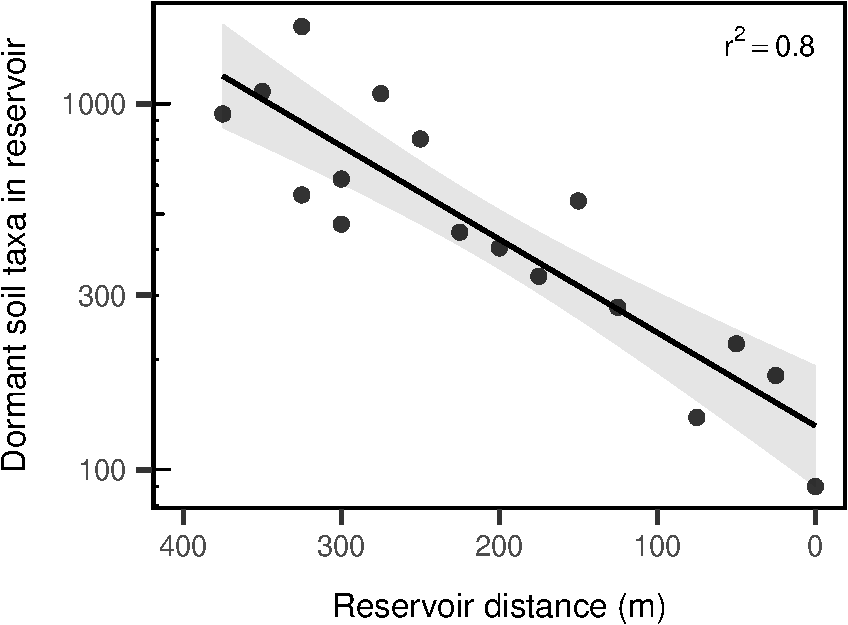
\includegraphics{ReservoirGradient_files/figure-latex/plot_transient-1} \end{center}

\begin{Shaded}
\begin{Highlighting}[]
\CommentTok{# plot_grid(alpha.fig, }
\CommentTok{#           similarity.plot, }
\CommentTok{#           pcoa.fig + , }
\CommentTok{#           transient.plot,}
\CommentTok{#           align = "hv", axis = "tlbr",}
\CommentTok{#           labels = "auto", ncol = 2) +}
\CommentTok{#   ggsave("figures/large_panel.pdf", width = 12, height = 8)}
\end{Highlighting}
\end{Shaded}

\section{What is the fate of soil-derived taxa in the
reservoir?}\label{what-is-the-fate-of-soil-derived-taxa-in-the-reservoir}

So, we observe that most soil-derived taxa appear to decay once they
enter the reservoir. Do any soil-derived taxa persist in the active
bacterial community of the reservoir and do they rise to high relative
abundances?

\begin{Shaded}
\begin{Highlighting}[]
\CommentTok{# identify otus in soil samples and lake samples}
\NormalTok{in.soil <-}\StringTok{ }\NormalTok{OTUs[, }\KeywordTok{which}\NormalTok{(}\KeywordTok{colSums}\NormalTok{(OTUs[}\KeywordTok{c}\NormalTok{(}\DecValTok{1}\OperatorTok{:}\DecValTok{3}\NormalTok{),]) }\OperatorTok{>}\StringTok{ }\DecValTok{0}\NormalTok{ )]}
\CommentTok{#in.lake <- OTUs[, which(colSums(OTUs[-c(1:3),]) > 0)]}

\CommentTok{# isolate just the rna water samples and convert to presence-absence}
\NormalTok{in.lake.rna <-}\StringTok{ }\NormalTok{OTUs[}\KeywordTok{which}\NormalTok{(design}\OperatorTok{$}\NormalTok{molecule }\OperatorTok{==}\StringTok{ "RNA"} \OperatorTok{&}\StringTok{ }\NormalTok{design}\OperatorTok{$}\NormalTok{type }\OperatorTok{==}\StringTok{ "water"}\NormalTok{), ]}
\NormalTok{in.lake.rna.pa <-}\StringTok{ }\NormalTok{(in.lake.rna }\OperatorTok{>}\StringTok{ }\DecValTok{0}\NormalTok{) }\OperatorTok{*}\StringTok{ }\DecValTok{1}

\CommentTok{# define the 'core' taxa as otus present in 50% of samples}
\NormalTok{in.lake.core <-}\StringTok{ }\NormalTok{w.dna[, }\KeywordTok{which}\NormalTok{((}\KeywordTok{colSums}\NormalTok{(in.lake.rna.pa) }\OperatorTok{/}\StringTok{ }\KeywordTok{nrow}\NormalTok{(in.lake.rna.pa)) }\OperatorTok{>=}\StringTok{ }\FloatTok{0.75}\NormalTok{)]}

\CommentTok{# of the core, how many are also in the soil samples?}
\NormalTok{in.lake.core.from.soils <-}\StringTok{ }\NormalTok{in.lake.core[, }\KeywordTok{intersect}\NormalTok{(}\KeywordTok{colnames}\NormalTok{(in.lake.core), }\KeywordTok{colnames}\NormalTok{(in.soil))]}

\CommentTok{# of the core which are not in the soil samples}
\NormalTok{in.lake.core.not.soils <-}\StringTok{ }\NormalTok{in.lake.core[, }\KeywordTok{setdiff}\NormalTok{(}\KeywordTok{colnames}\NormalTok{(in.lake.core), }\KeywordTok{colnames}\NormalTok{(in.soil))]}

\CommentTok{# Find the relative abundance of the core taxa and prepare data frame to plot}
\NormalTok{in.lake.core.from.soils.REL <-}\StringTok{ }\NormalTok{in.lake.core.from.soils }\OperatorTok{/}\StringTok{ }\KeywordTok{rowSums}\NormalTok{(w.dna)}

\NormalTok{in.soil.to.plot <-}\StringTok{ }\KeywordTok{as.data.frame}\NormalTok{(in.lake.core.from.soils.REL) }\OperatorTok\StringTok{ }
\StringTok{  }\KeywordTok{rownames_to_column}\NormalTok{(}\StringTok{"sample_ID"}\NormalTok{) }\OperatorTok\StringTok{ }
\StringTok{  }\KeywordTok{gather}\NormalTok{(otu_id, rel_abundance, }\OperatorTok{-}\NormalTok{sample_ID) }\OperatorTok\StringTok{ }
\StringTok{  }\KeywordTok{left_join}\NormalTok{(}\KeywordTok{rownames_to_column}\NormalTok{(design.dna, }\StringTok{"sample_ID"}\NormalTok{)) }\OperatorTok\StringTok{ }
\StringTok{  }\KeywordTok{add_column}\NormalTok{(}\DataTypeTok{found =} \StringTok{"soils"}\NormalTok{)}

\NormalTok{in.lake.core.not.soils.REL <-}\StringTok{ }\NormalTok{in.lake.core.not.soils }\OperatorTok{/}\StringTok{ }\KeywordTok{rowSums}\NormalTok{(w.dna)}

\NormalTok{in.lake.to.plot <-}\StringTok{ }\KeywordTok{as.data.frame}\NormalTok{(in.lake.core.not.soils.REL) }\OperatorTok\StringTok{ }
\StringTok{  }\KeywordTok{rownames_to_column}\NormalTok{(}\StringTok{"sample_ID"}\NormalTok{) }\OperatorTok\StringTok{ }
\StringTok{  }\KeywordTok{gather}\NormalTok{(otu_id, rel_abundance, }\OperatorTok{-}\NormalTok{sample_ID) }\OperatorTok\StringTok{ }
\StringTok{  }\KeywordTok{left_join}\NormalTok{(}\KeywordTok{rownames_to_column}\NormalTok{(design.dna, }\StringTok{"sample_ID"}\NormalTok{)) }\OperatorTok\StringTok{ }
\StringTok{  }\KeywordTok{add_column}\NormalTok{(}\DataTypeTok{found =} \StringTok{"lake"}\NormalTok{)}
\end{Highlighting}
\end{Shaded}

Now, lets plot the abundances of the OTUs across the reservoir and split
them up into whether they were recovered in soils or not.

\begin{Shaded}
\begin{Highlighting}[]
\KeywordTok{bind_rows}\NormalTok{(in.soil.to.plot, in.lake.to.plot) }\OperatorTok\StringTok{ }
\StringTok{  }\KeywordTok{ggplot}\NormalTok{(}\KeywordTok{aes}\NormalTok{(}\DataTypeTok{x =}\NormalTok{ distance, }\DataTypeTok{y =}\NormalTok{ rel_abundance, }\DataTypeTok{group =}\NormalTok{ otu_id)) }\OperatorTok{+}\StringTok{ }
\StringTok{  }\KeywordTok{labs}\NormalTok{(}\DataTypeTok{x =} \StringTok{"Reservoir distance (m)"}\NormalTok{, }
       \DataTypeTok{y =} \StringTok{"OTU relative abundance"}\NormalTok{) }\OperatorTok{+}
\StringTok{  }\KeywordTok{geom_line}\NormalTok{(}\DataTypeTok{alpha =} \FloatTok{0.25}\NormalTok{, }\DataTypeTok{stat =} \StringTok{"smooth"}\NormalTok{, }\DataTypeTok{method =} \StringTok{"lm"}\NormalTok{, }\DataTypeTok{se =}\NormalTok{ F, }\DataTypeTok{show.legend =}\NormalTok{ F) }\OperatorTok{+}
\StringTok{  }\KeywordTok{scale_y_log10}\NormalTok{() }\OperatorTok{+}
\StringTok{  }\KeywordTok{scale_x_reverse}\NormalTok{() }\OperatorTok{+}\StringTok{ }
\StringTok{  }\KeywordTok{facet_wrap}\NormalTok{(}\OperatorTok{~}\StringTok{ }\NormalTok{found, }\DataTypeTok{ncol =} \DecValTok{1}\NormalTok{, }
             \DataTypeTok{labeller =} \KeywordTok{as_labeller}\NormalTok{(}\KeywordTok{c}\NormalTok{(}
               \StringTok{`}\DataTypeTok{lake}\StringTok{`}\NormalTok{ =}\StringTok{ "Undetected in soils"}\NormalTok{,}
               \StringTok{`}\DataTypeTok{soils}\StringTok{`}\NormalTok{ =}\StringTok{ "Present in soils"}\NormalTok{)))}
\end{Highlighting}
\end{Shaded}

\begin{verbatim}
## Warning: Transformation introduced infinite values in continuous y-axis
\end{verbatim}

\begin{verbatim}
## Warning: Removed 59 rows containing non-finite values (stat_smooth).
\end{verbatim}

\begin{center}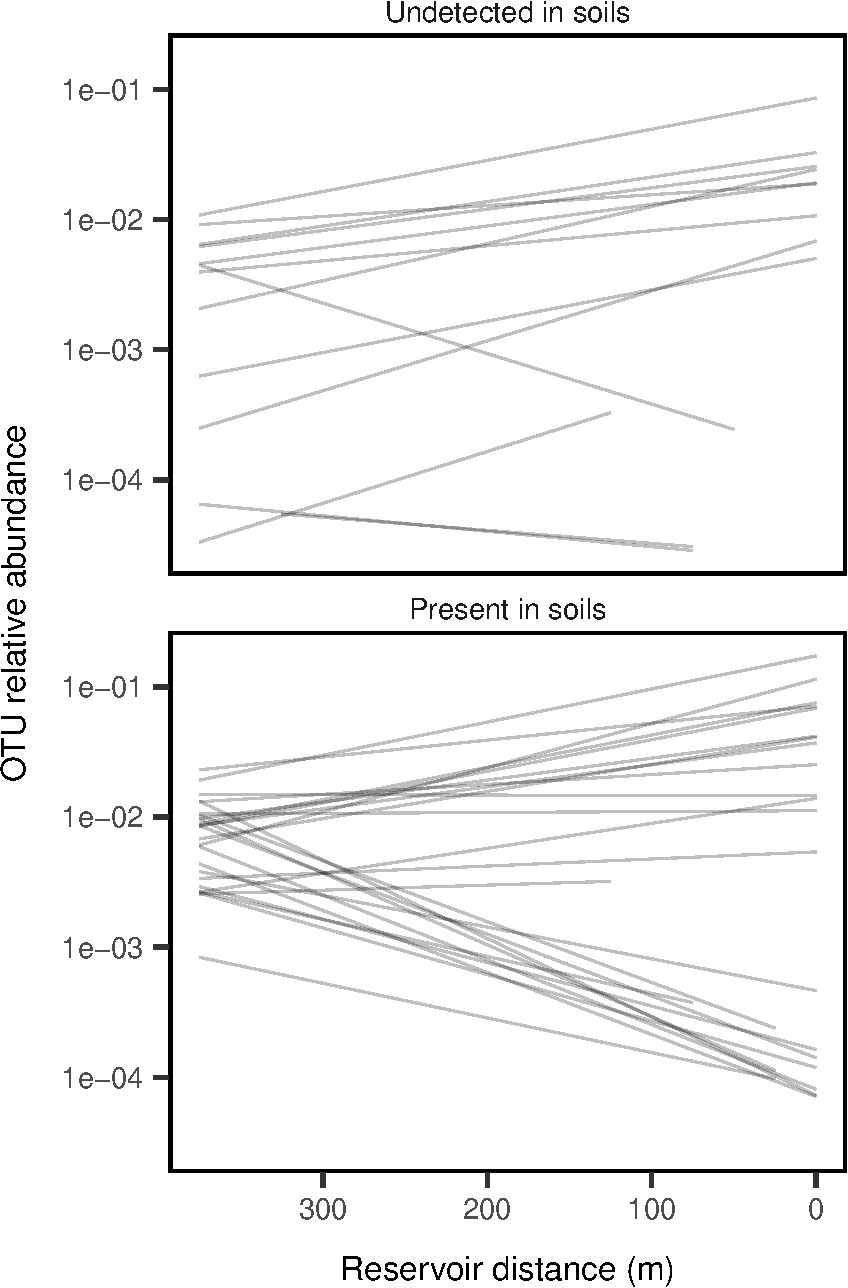
\includegraphics{ReservoirGradient_files/figure-latex/coreplot-1} \end{center}

From this figure, we note a few important points. First, we observe that
core reservoir taxa that are not detected in the soil samples tend to
increase in relative abundance along the reservoir transect. We also
note that for the taxa that are present in the soil samples, some tend
to increase drastically, while others tend to increase, along the
transect. This suggests that there may be two classes of soil-derived
OTUs that contribute to reservoir bacterial diversity:\\
- taxa where the reservoir is a sink (i.e., maintained via mass effects
from the soils) - aquatic taxa seeded by populations stored in the soils

\begin{Shaded}
\begin{Highlighting}[]
\CommentTok{# model distance effect on rel abundance to get slope and pval}
\NormalTok{soil.core.mods <-}\StringTok{ }\KeywordTok{apply}\NormalTok{(in.lake.core.from.soils.REL, }\DataTypeTok{MARGIN =} \DecValTok{2}\NormalTok{, }
    \DataTypeTok{FUN =} \ControlFlowTok{function}\NormalTok{(x) }\KeywordTok{summary}\NormalTok{(}\KeywordTok{lm}\NormalTok{(x }\OperatorTok{~}\StringTok{ }\NormalTok{design.dna}\OperatorTok{$}\NormalTok{distance))}\OperatorTok{$}\NormalTok{coefficients[}\DecValTok{2}\NormalTok{,}\KeywordTok{c}\NormalTok{(}\DecValTok{1}\NormalTok{,}\DecValTok{4}\NormalTok{)])}
\KeywordTok{rownames}\NormalTok{(soil.core.mods) <-}\StringTok{ }\KeywordTok{c}\NormalTok{(}\StringTok{"slope"}\NormalTok{, }\StringTok{"pval"}\NormalTok{)}

\CommentTok{# classify otus as significantly increasing or decreasing along reservoir}
\NormalTok{soil.core.decreasing <-}\StringTok{ }\KeywordTok{as.data.frame}\NormalTok{(}\KeywordTok{t}\NormalTok{(soil.core.mods)) }\OperatorTok\StringTok{ }
\StringTok{  }\KeywordTok{rownames_to_column}\NormalTok{(}\StringTok{"OTU"}\NormalTok{) }\OperatorTok\StringTok{ }
\StringTok{  }\KeywordTok{filter}\NormalTok{(slope }\OperatorTok{>}\StringTok{ }\DecValTok{0}\NormalTok{) }\OperatorTok\StringTok{   }\CommentTok{# rel abund decreases toward dam}
\StringTok{  }\KeywordTok{left_join}\NormalTok{(OTU.tax)}
\end{Highlighting}
\end{Shaded}

\begin{verbatim}
## Warning: Column `OTU` joining character vector and factor, coercing into
## character vector
\end{verbatim}

\begin{Shaded}
\begin{Highlighting}[]
\NormalTok{soil.core.increasing <-}\StringTok{ }\KeywordTok{as.data.frame}\NormalTok{(}\KeywordTok{t}\NormalTok{(soil.core.mods)) }\OperatorTok\StringTok{ }
\StringTok{  }\KeywordTok{rownames_to_column}\NormalTok{(}\StringTok{"OTU"}\NormalTok{) }\OperatorTok\StringTok{ }
\StringTok{  }\KeywordTok{filter}\NormalTok{(slope }\OperatorTok{<}\StringTok{ }\DecValTok{0}\NormalTok{) }\OperatorTok\StringTok{   }\CommentTok{# rel abund increases toward dam}
\StringTok{  }\KeywordTok{left_join}\NormalTok{(OTU.tax)}
\end{Highlighting}
\end{Shaded}

\begin{verbatim}
## Warning: Column `OTU` joining character vector and factor, coercing into
## character vector
\end{verbatim}

\begin{Shaded}
\begin{Highlighting}[]
\NormalTok{nonsoil.core.mods <-}\StringTok{ }\KeywordTok{apply}\NormalTok{(in.lake.core.not.soils.REL, }\DataTypeTok{MARGIN =} \DecValTok{2}\NormalTok{, }
    \DataTypeTok{FUN =} \ControlFlowTok{function}\NormalTok{(x) }\KeywordTok{summary}\NormalTok{(}\KeywordTok{lm}\NormalTok{(x }\OperatorTok{~}\StringTok{ }\NormalTok{design.dna}\OperatorTok{$}\NormalTok{distance))}\OperatorTok{$}\NormalTok{coefficients[}\DecValTok{2}\NormalTok{,}\KeywordTok{c}\NormalTok{(}\DecValTok{1}\NormalTok{,}\DecValTok{4}\NormalTok{)])}
\KeywordTok{rownames}\NormalTok{(nonsoil.core.mods) <-}\StringTok{ }\KeywordTok{c}\NormalTok{(}\StringTok{"slope"}\NormalTok{, }\StringTok{"pval"}\NormalTok{)}
\NormalTok{nonsoil.core.decreasing <-}\StringTok{ }\KeywordTok{as.data.frame}\NormalTok{(}\KeywordTok{t}\NormalTok{(nonsoil.core.mods)) }\OperatorTok\StringTok{ }
\StringTok{  }\KeywordTok{rownames_to_column}\NormalTok{(}\StringTok{"OTU"}\NormalTok{) }\OperatorTok\StringTok{ }
\StringTok{  }\KeywordTok{filter}\NormalTok{(slope }\OperatorTok{>}\StringTok{ }\DecValTok{0}\NormalTok{) }\OperatorTok\StringTok{   }\CommentTok{# rel abund decreases toward dam}
\StringTok{  }\KeywordTok{left_join}\NormalTok{(OTU.tax)}
\end{Highlighting}
\end{Shaded}

\begin{verbatim}
## Warning: Column `OTU` joining character vector and factor, coercing into
## character vector
\end{verbatim}

\begin{Shaded}
\begin{Highlighting}[]
\NormalTok{nonsoil.core.increasing <-}\StringTok{ }\KeywordTok{as.data.frame}\NormalTok{(}\KeywordTok{t}\NormalTok{(nonsoil.core.mods)) }\OperatorTok\StringTok{ }
\StringTok{  }\KeywordTok{rownames_to_column}\NormalTok{(}\StringTok{"OTU"}\NormalTok{) }\OperatorTok\StringTok{ }
\StringTok{  }\KeywordTok{filter}\NormalTok{(slope }\OperatorTok{<}\StringTok{ }\DecValTok{0}\NormalTok{) }\OperatorTok\StringTok{   }\CommentTok{# rel abund increases toward dam}
\StringTok{  }\KeywordTok{left_join}\NormalTok{(OTU.tax)}
\end{Highlighting}
\end{Shaded}

\begin{verbatim}
## Warning: Column `OTU` joining character vector and factor, coercing into
## character vector
\end{verbatim}

Now we will visualize the significant taxa

\begin{Shaded}
\begin{Highlighting}[]
\KeywordTok{pander}\NormalTok{(nonsoil.core.decreasing, }\DataTypeTok{caption =} \StringTok{"Core taxa not found in soils that get rarer along the transect."}\NormalTok{)}
\end{Highlighting}
\end{Shaded}

\begin{longtable}[]{@{}ccccc@{}}
\caption{Core taxa not found in soils that get rarer along the transect.
(continued below)}\tabularnewline
\toprule
\begin{minipage}[b]{0.13\columnwidth}\centering\strut
OTU\strut
\end{minipage} & \begin{minipage}[b]{0.14\columnwidth}\centering\strut
slope\strut
\end{minipage} & \begin{minipage}[b]{0.12\columnwidth}\centering\strut
pval\strut
\end{minipage} & \begin{minipage}[b]{0.13\columnwidth}\centering\strut
Domain\strut
\end{minipage} & \begin{minipage}[b]{0.19\columnwidth}\centering\strut
Phylum\strut
\end{minipage}\tabularnewline
\midrule
\endfirsthead
\toprule
\begin{minipage}[b]{0.13\columnwidth}\centering\strut
OTU\strut
\end{minipage} & \begin{minipage}[b]{0.14\columnwidth}\centering\strut
slope\strut
\end{minipage} & \begin{minipage}[b]{0.12\columnwidth}\centering\strut
pval\strut
\end{minipage} & \begin{minipage}[b]{0.13\columnwidth}\centering\strut
Domain\strut
\end{minipage} & \begin{minipage}[b]{0.19\columnwidth}\centering\strut
Phylum\strut
\end{minipage}\tabularnewline
\midrule
\endhead
\begin{minipage}[t]{0.13\columnwidth}\centering\strut
Otu00020\strut
\end{minipage} & \begin{minipage}[t]{0.14\columnwidth}\centering\strut
4.933e-07\strut
\end{minipage} & \begin{minipage}[t]{0.12\columnwidth}\centering\strut
0.9784\strut
\end{minipage} & \begin{minipage}[t]{0.13\columnwidth}\centering\strut
Bacteria\strut
\end{minipage} & \begin{minipage}[t]{0.19\columnwidth}\centering\strut
Proteobacteria\strut
\end{minipage}\tabularnewline
\begin{minipage}[t]{0.13\columnwidth}\centering\strut
Otu00138\strut
\end{minipage} & \begin{minipage}[t]{0.14\columnwidth}\centering\strut
3.152e-05\strut
\end{minipage} & \begin{minipage}[t]{0.12\columnwidth}\centering\strut
0.04589\strut
\end{minipage} & \begin{minipage}[t]{0.13\columnwidth}\centering\strut
Bacteria\strut
\end{minipage} & \begin{minipage}[t]{0.19\columnwidth}\centering\strut
Firmicutes\strut
\end{minipage}\tabularnewline
\begin{minipage}[t]{0.13\columnwidth}\centering\strut
Otu01010\strut
\end{minipage} & \begin{minipage}[t]{0.14\columnwidth}\centering\strut
1.364e-08\strut
\end{minipage} & \begin{minipage}[t]{0.12\columnwidth}\centering\strut
0.8511\strut
\end{minipage} & \begin{minipage}[t]{0.13\columnwidth}\centering\strut
Bacteria\strut
\end{minipage} & \begin{minipage}[t]{0.19\columnwidth}\centering\strut
Actinobacteria\strut
\end{minipage}\tabularnewline
\begin{minipage}[t]{0.13\columnwidth}\centering\strut
Otu01055\strut
\end{minipage} & \begin{minipage}[t]{0.14\columnwidth}\centering\strut
6.268e-08\strut
\end{minipage} & \begin{minipage}[t]{0.12\columnwidth}\centering\strut
0.25\strut
\end{minipage} & \begin{minipage}[t]{0.13\columnwidth}\centering\strut
Bacteria\strut
\end{minipage} & \begin{minipage}[t]{0.19\columnwidth}\centering\strut
Actinobacteria\strut
\end{minipage}\tabularnewline
\bottomrule
\end{longtable}

\begin{longtable}[]{@{}ccc@{}}
\caption{Table continues below}\tabularnewline
\toprule
\begin{minipage}[b]{0.27\columnwidth}\centering\strut
Class\strut
\end{minipage} & \begin{minipage}[b]{0.23\columnwidth}\centering\strut
Order\strut
\end{minipage} & \begin{minipage}[b]{0.23\columnwidth}\centering\strut
Family\strut
\end{minipage}\tabularnewline
\midrule
\endfirsthead
\toprule
\begin{minipage}[b]{0.27\columnwidth}\centering\strut
Class\strut
\end{minipage} & \begin{minipage}[b]{0.23\columnwidth}\centering\strut
Order\strut
\end{minipage} & \begin{minipage}[b]{0.23\columnwidth}\centering\strut
Family\strut
\end{minipage}\tabularnewline
\midrule
\endhead
\begin{minipage}[t]{0.27\columnwidth}\centering\strut
Betaproteobacteria\strut
\end{minipage} & \begin{minipage}[t]{0.23\columnwidth}\centering\strut
Burkholderiales\strut
\end{minipage} & \begin{minipage}[t]{0.23\columnwidth}\centering\strut
Alcaligenaceae\strut
\end{minipage}\tabularnewline
\begin{minipage}[t]{0.27\columnwidth}\centering\strut
Bacilli\strut
\end{minipage} & \begin{minipage}[t]{0.23\columnwidth}\centering\strut
Bacillales\strut
\end{minipage} & \begin{minipage}[t]{0.23\columnwidth}\centering\strut
Bacillaceae\_1\strut
\end{minipage}\tabularnewline
\begin{minipage}[t]{0.27\columnwidth}\centering\strut
Actinobacteria\strut
\end{minipage} & \begin{minipage}[t]{0.23\columnwidth}\centering\strut
Actinomycetales\strut
\end{minipage} & \begin{minipage}[t]{0.23\columnwidth}\centering\strut
Dermabacteraceae\strut
\end{minipage}\tabularnewline
\begin{minipage}[t]{0.27\columnwidth}\centering\strut
Actinobacteria\strut
\end{minipage} & \begin{minipage}[t]{0.23\columnwidth}\centering\strut
Actinomycetales\strut
\end{minipage} & \begin{minipage}[t]{0.23\columnwidth}\centering\strut
Dietziaceae\strut
\end{minipage}\tabularnewline
\bottomrule
\end{longtable}

\begin{longtable}[]{@{}c@{}}
\toprule
\begin{minipage}[b]{0.39\columnwidth}\centering\strut
Genus\strut
\end{minipage}\tabularnewline
\midrule
\endhead
\begin{minipage}[t]{0.39\columnwidth}\centering\strut
Alcaligenaceae\_unclassified\strut
\end{minipage}\tabularnewline
\begin{minipage}[t]{0.39\columnwidth}\centering\strut
Bacillus\strut
\end{minipage}\tabularnewline
\begin{minipage}[t]{0.39\columnwidth}\centering\strut
Brachybacterium\strut
\end{minipage}\tabularnewline
\begin{minipage}[t]{0.39\columnwidth}\centering\strut
Dietzia\strut
\end{minipage}\tabularnewline
\bottomrule
\end{longtable}

\begin{Shaded}
\begin{Highlighting}[]
\KeywordTok{pander}\NormalTok{(nonsoil.core.increasing, }\DataTypeTok{caption =} \StringTok{"Core taxa not found in soils that get more common along the transect."}\NormalTok{)}
\end{Highlighting}
\end{Shaded}

\begin{longtable}[]{@{}ccccc@{}}
\caption{Core taxa not found in soils that get more common along the
transect. (continued below)}\tabularnewline
\toprule
\begin{minipage}[b]{0.13\columnwidth}\centering\strut
OTU\strut
\end{minipage} & \begin{minipage}[b]{0.16\columnwidth}\centering\strut
slope\strut
\end{minipage} & \begin{minipage}[b]{0.14\columnwidth}\centering\strut
pval\strut
\end{minipage} & \begin{minipage}[b]{0.13\columnwidth}\centering\strut
Domain\strut
\end{minipage} & \begin{minipage}[b]{0.27\columnwidth}\centering\strut
Phylum\strut
\end{minipage}\tabularnewline
\midrule
\endfirsthead
\toprule
\begin{minipage}[b]{0.13\columnwidth}\centering\strut
OTU\strut
\end{minipage} & \begin{minipage}[b]{0.16\columnwidth}\centering\strut
slope\strut
\end{minipage} & \begin{minipage}[b]{0.14\columnwidth}\centering\strut
pval\strut
\end{minipage} & \begin{minipage}[b]{0.13\columnwidth}\centering\strut
Domain\strut
\end{minipage} & \begin{minipage}[b]{0.27\columnwidth}\centering\strut
Phylum\strut
\end{minipage}\tabularnewline
\midrule
\endhead
\begin{minipage}[t]{0.13\columnwidth}\centering\strut
Otu00004\strut
\end{minipage} & \begin{minipage}[t]{0.16\columnwidth}\centering\strut
-0.0001379\strut
\end{minipage} & \begin{minipage}[t]{0.14\columnwidth}\centering\strut
3.031e-06\strut
\end{minipage} & \begin{minipage}[t]{0.13\columnwidth}\centering\strut
Bacteria\strut
\end{minipage} & \begin{minipage}[t]{0.27\columnwidth}\centering\strut
Actinobacteria\strut
\end{minipage}\tabularnewline
\begin{minipage}[t]{0.13\columnwidth}\centering\strut
Otu00007\strut
\end{minipage} & \begin{minipage}[t]{0.16\columnwidth}\centering\strut
-3.822e-06\strut
\end{minipage} & \begin{minipage}[t]{0.14\columnwidth}\centering\strut
0.704\strut
\end{minipage} & \begin{minipage}[t]{0.13\columnwidth}\centering\strut
Bacteria\strut
\end{minipage} & \begin{minipage}[t]{0.27\columnwidth}\centering\strut
Proteobacteria\strut
\end{minipage}\tabularnewline
\begin{minipage}[t]{0.13\columnwidth}\centering\strut
Otu00023\strut
\end{minipage} & \begin{minipage}[t]{0.16\columnwidth}\centering\strut
-3.269e-07\strut
\end{minipage} & \begin{minipage}[t]{0.14\columnwidth}\centering\strut
0.7409\strut
\end{minipage} & \begin{minipage}[t]{0.13\columnwidth}\centering\strut
Bacteria\strut
\end{minipage} & \begin{minipage}[t]{0.27\columnwidth}\centering\strut
Proteobacteria\strut
\end{minipage}\tabularnewline
\begin{minipage}[t]{0.13\columnwidth}\centering\strut
Otu00025\strut
\end{minipage} & \begin{minipage}[t]{0.16\columnwidth}\centering\strut
-5.193e-05\strut
\end{minipage} & \begin{minipage}[t]{0.14\columnwidth}\centering\strut
0.000563\strut
\end{minipage} & \begin{minipage}[t]{0.13\columnwidth}\centering\strut
Bacteria\strut
\end{minipage} & \begin{minipage}[t]{0.27\columnwidth}\centering\strut
Actinobacteria\strut
\end{minipage}\tabularnewline
\begin{minipage}[t]{0.13\columnwidth}\centering\strut
Otu00032\strut
\end{minipage} & \begin{minipage}[t]{0.16\columnwidth}\centering\strut
-1.799e-05\strut
\end{minipage} & \begin{minipage}[t]{0.14\columnwidth}\centering\strut
0.2422\strut
\end{minipage} & \begin{minipage}[t]{0.13\columnwidth}\centering\strut
Bacteria\strut
\end{minipage} & \begin{minipage}[t]{0.27\columnwidth}\centering\strut
Bacteroidetes\strut
\end{minipage}\tabularnewline
\begin{minipage}[t]{0.13\columnwidth}\centering\strut
Otu00038\strut
\end{minipage} & \begin{minipage}[t]{0.16\columnwidth}\centering\strut
-4.082e-05\strut
\end{minipage} & \begin{minipage}[t]{0.14\columnwidth}\centering\strut
0.0004677\strut
\end{minipage} & \begin{minipage}[t]{0.13\columnwidth}\centering\strut
Bacteria\strut
\end{minipage} & \begin{minipage}[t]{0.27\columnwidth}\centering\strut
Actinobacteria\strut
\end{minipage}\tabularnewline
\begin{minipage}[t]{0.13\columnwidth}\centering\strut
Otu00040\strut
\end{minipage} & \begin{minipage}[t]{0.16\columnwidth}\centering\strut
-3.681e-05\strut
\end{minipage} & \begin{minipage}[t]{0.14\columnwidth}\centering\strut
1.522e-05\strut
\end{minipage} & \begin{minipage}[t]{0.13\columnwidth}\centering\strut
Bacteria\strut
\end{minipage} & \begin{minipage}[t]{0.27\columnwidth}\centering\strut
Proteobacteria\strut
\end{minipage}\tabularnewline
\begin{minipage}[t]{0.13\columnwidth}\centering\strut
Otu00118\strut
\end{minipage} & \begin{minipage}[t]{0.16\columnwidth}\centering\strut
-7.165e-06\strut
\end{minipage} & \begin{minipage}[t]{0.14\columnwidth}\centering\strut
0.01503\strut
\end{minipage} & \begin{minipage}[t]{0.13\columnwidth}\centering\strut
Bacteria\strut
\end{minipage} & \begin{minipage}[t]{0.27\columnwidth}\centering\strut
Actinobacteria\strut
\end{minipage}\tabularnewline
\begin{minipage}[t]{0.13\columnwidth}\centering\strut
Otu00156\strut
\end{minipage} & \begin{minipage}[t]{0.16\columnwidth}\centering\strut
-9.057e-06\strut
\end{minipage} & \begin{minipage}[t]{0.14\columnwidth}\centering\strut
0.0002607\strut
\end{minipage} & \begin{minipage}[t]{0.13\columnwidth}\centering\strut
Bacteria\strut
\end{minipage} & \begin{minipage}[t]{0.27\columnwidth}\centering\strut
Bacteria\_unclassified\strut
\end{minipage}\tabularnewline
\bottomrule
\end{longtable}

\begin{longtable}[]{@{}cc@{}}
\caption{Table continues below}\tabularnewline
\toprule
\begin{minipage}[b]{0.38\columnwidth}\centering\strut
Class\strut
\end{minipage} & \begin{minipage}[b]{0.38\columnwidth}\centering\strut
Order\strut
\end{minipage}\tabularnewline
\midrule
\endfirsthead
\toprule
\begin{minipage}[b]{0.38\columnwidth}\centering\strut
Class\strut
\end{minipage} & \begin{minipage}[b]{0.38\columnwidth}\centering\strut
Order\strut
\end{minipage}\tabularnewline
\midrule
\endhead
\begin{minipage}[t]{0.38\columnwidth}\centering\strut
Actinobacteria\strut
\end{minipage} & \begin{minipage}[t]{0.38\columnwidth}\centering\strut
Actinomycetales\strut
\end{minipage}\tabularnewline
\begin{minipage}[t]{0.38\columnwidth}\centering\strut
Betaproteobacteria\strut
\end{minipage} & \begin{minipage}[t]{0.38\columnwidth}\centering\strut
Burkholderiales\strut
\end{minipage}\tabularnewline
\begin{minipage}[t]{0.38\columnwidth}\centering\strut
Gammaproteobacteria\strut
\end{minipage} & \begin{minipage}[t]{0.38\columnwidth}\centering\strut
Pseudomonadales\strut
\end{minipage}\tabularnewline
\begin{minipage}[t]{0.38\columnwidth}\centering\strut
Actinobacteria\strut
\end{minipage} & \begin{minipage}[t]{0.38\columnwidth}\centering\strut
Actinomycetales\strut
\end{minipage}\tabularnewline
\begin{minipage}[t]{0.38\columnwidth}\centering\strut
Bacteroidetes\_unclassified\strut
\end{minipage} & \begin{minipage}[t]{0.38\columnwidth}\centering\strut
Bacteroidetes\_unclassified\strut
\end{minipage}\tabularnewline
\begin{minipage}[t]{0.38\columnwidth}\centering\strut
Actinobacteria\strut
\end{minipage} & \begin{minipage}[t]{0.38\columnwidth}\centering\strut
Actinomycetales\strut
\end{minipage}\tabularnewline
\begin{minipage}[t]{0.38\columnwidth}\centering\strut
Alphaproteobacteria\strut
\end{minipage} & \begin{minipage}[t]{0.38\columnwidth}\centering\strut
Rhodospirillales\strut
\end{minipage}\tabularnewline
\begin{minipage}[t]{0.38\columnwidth}\centering\strut
Actinobacteria\strut
\end{minipage} & \begin{minipage}[t]{0.38\columnwidth}\centering\strut
Actinobacteria\_unclassified\strut
\end{minipage}\tabularnewline
\begin{minipage}[t]{0.38\columnwidth}\centering\strut
Bacteria\_unclassified\strut
\end{minipage} & \begin{minipage}[t]{0.38\columnwidth}\centering\strut
Bacteria\_unclassified\strut
\end{minipage}\tabularnewline
\bottomrule
\end{longtable}

\begin{longtable}[]{@{}cc@{}}
\toprule
\begin{minipage}[b]{0.41\columnwidth}\centering\strut
Family\strut
\end{minipage} & \begin{minipage}[b]{0.42\columnwidth}\centering\strut
Genus\strut
\end{minipage}\tabularnewline
\midrule
\endhead
\begin{minipage}[t]{0.41\columnwidth}\centering\strut
Actinomycetales\_unclassified\strut
\end{minipage} & \begin{minipage}[t]{0.42\columnwidth}\centering\strut
Actinomycetales\_unclassified\strut
\end{minipage}\tabularnewline
\begin{minipage}[t]{0.41\columnwidth}\centering\strut
Burkholderiaceae\strut
\end{minipage} & \begin{minipage}[t]{0.42\columnwidth}\centering\strut
Polynucleobacter\strut
\end{minipage}\tabularnewline
\begin{minipage}[t]{0.41\columnwidth}\centering\strut
Moraxellaceae\strut
\end{minipage} & \begin{minipage}[t]{0.42\columnwidth}\centering\strut
Acinetobacter\strut
\end{minipage}\tabularnewline
\begin{minipage}[t]{0.41\columnwidth}\centering\strut
Microbacteriaceae\strut
\end{minipage} & \begin{minipage}[t]{0.42\columnwidth}\centering\strut
Microbacteriaceae\_unclassified\strut
\end{minipage}\tabularnewline
\begin{minipage}[t]{0.41\columnwidth}\centering\strut
Bacteroidetes\_unclassified\strut
\end{minipage} & \begin{minipage}[t]{0.42\columnwidth}\centering\strut
Bacteroidetes\_unclassified\strut
\end{minipage}\tabularnewline
\begin{minipage}[t]{0.41\columnwidth}\centering\strut
Actinomycetales\_unclassified\strut
\end{minipage} & \begin{minipage}[t]{0.42\columnwidth}\centering\strut
Actinomycetales\_unclassified\strut
\end{minipage}\tabularnewline
\begin{minipage}[t]{0.41\columnwidth}\centering\strut
Acetobacteraceae\strut
\end{minipage} & \begin{minipage}[t]{0.42\columnwidth}\centering\strut
Roseomonas\strut
\end{minipage}\tabularnewline
\begin{minipage}[t]{0.41\columnwidth}\centering\strut
Actinobacteria\_unclassified\strut
\end{minipage} & \begin{minipage}[t]{0.42\columnwidth}\centering\strut
Actinobacteria\_unclassified\strut
\end{minipage}\tabularnewline
\begin{minipage}[t]{0.41\columnwidth}\centering\strut
Bacteria\_unclassified\strut
\end{minipage} & \begin{minipage}[t]{0.42\columnwidth}\centering\strut
Bacteria\_unclassified\strut
\end{minipage}\tabularnewline
\bottomrule
\end{longtable}

\begin{Shaded}
\begin{Highlighting}[]
\KeywordTok{pander}\NormalTok{(soil.core.decreasing, }\DataTypeTok{caption =} \StringTok{"Core taxa found in soils that get rarer along the transect."}\NormalTok{)}
\end{Highlighting}
\end{Shaded}

\begin{longtable}[]{@{}ccccc@{}}
\caption{Core taxa found in soils that get rarer along the transect.
(continued below)}\tabularnewline
\toprule
\begin{minipage}[b]{0.13\columnwidth}\centering\strut
OTU\strut
\end{minipage} & \begin{minipage}[b]{0.14\columnwidth}\centering\strut
slope\strut
\end{minipage} & \begin{minipage}[b]{0.12\columnwidth}\centering\strut
pval\strut
\end{minipage} & \begin{minipage}[b]{0.13\columnwidth}\centering\strut
Domain\strut
\end{minipage} & \begin{minipage}[b]{0.20\columnwidth}\centering\strut
Phylum\strut
\end{minipage}\tabularnewline
\midrule
\endfirsthead
\toprule
\begin{minipage}[b]{0.13\columnwidth}\centering\strut
OTU\strut
\end{minipage} & \begin{minipage}[b]{0.14\columnwidth}\centering\strut
slope\strut
\end{minipage} & \begin{minipage}[b]{0.12\columnwidth}\centering\strut
pval\strut
\end{minipage} & \begin{minipage}[b]{0.13\columnwidth}\centering\strut
Domain\strut
\end{minipage} & \begin{minipage}[b]{0.20\columnwidth}\centering\strut
Phylum\strut
\end{minipage}\tabularnewline
\midrule
\endhead
\begin{minipage}[t]{0.13\columnwidth}\centering\strut
Otu00009\strut
\end{minipage} & \begin{minipage}[t]{0.14\columnwidth}\centering\strut
4.862e-05\strut
\end{minipage} & \begin{minipage}[t]{0.12\columnwidth}\centering\strut
0.06326\strut
\end{minipage} & \begin{minipage}[t]{0.13\columnwidth}\centering\strut
Bacteria\strut
\end{minipage} & \begin{minipage}[t]{0.20\columnwidth}\centering\strut
Proteobacteria\strut
\end{minipage}\tabularnewline
\begin{minipage}[t]{0.13\columnwidth}\centering\strut
Otu00012\strut
\end{minipage} & \begin{minipage}[t]{0.14\columnwidth}\centering\strut
7.397e-07\strut
\end{minipage} & \begin{minipage}[t]{0.12\columnwidth}\centering\strut
0.9069\strut
\end{minipage} & \begin{minipage}[t]{0.13\columnwidth}\centering\strut
Bacteria\strut
\end{minipage} & \begin{minipage}[t]{0.20\columnwidth}\centering\strut
Proteobacteria\strut
\end{minipage}\tabularnewline
\begin{minipage}[t]{0.13\columnwidth}\centering\strut
Otu00018\strut
\end{minipage} & \begin{minipage}[t]{0.14\columnwidth}\centering\strut
4.823e-05\strut
\end{minipage} & \begin{minipage}[t]{0.12\columnwidth}\centering\strut
0.02295\strut
\end{minipage} & \begin{minipage}[t]{0.13\columnwidth}\centering\strut
Bacteria\strut
\end{minipage} & \begin{minipage}[t]{0.20\columnwidth}\centering\strut
Proteobacteria\strut
\end{minipage}\tabularnewline
\begin{minipage}[t]{0.13\columnwidth}\centering\strut
Otu00022\strut
\end{minipage} & \begin{minipage}[t]{0.14\columnwidth}\centering\strut
9.926e-06\strut
\end{minipage} & \begin{minipage}[t]{0.12\columnwidth}\centering\strut
0.5565\strut
\end{minipage} & \begin{minipage}[t]{0.13\columnwidth}\centering\strut
Bacteria\strut
\end{minipage} & \begin{minipage}[t]{0.20\columnwidth}\centering\strut
Verrucomicrobia\strut
\end{minipage}\tabularnewline
\begin{minipage}[t]{0.13\columnwidth}\centering\strut
Otu00028\strut
\end{minipage} & \begin{minipage}[t]{0.14\columnwidth}\centering\strut
2.89e-05\strut
\end{minipage} & \begin{minipage}[t]{0.12\columnwidth}\centering\strut
0.06155\strut
\end{minipage} & \begin{minipage}[t]{0.13\columnwidth}\centering\strut
Bacteria\strut
\end{minipage} & \begin{minipage}[t]{0.20\columnwidth}\centering\strut
Proteobacteria\strut
\end{minipage}\tabularnewline
\begin{minipage}[t]{0.13\columnwidth}\centering\strut
Otu00030\strut
\end{minipage} & \begin{minipage}[t]{0.14\columnwidth}\centering\strut
1.849e-05\strut
\end{minipage} & \begin{minipage}[t]{0.12\columnwidth}\centering\strut
0.07112\strut
\end{minipage} & \begin{minipage}[t]{0.13\columnwidth}\centering\strut
Bacteria\strut
\end{minipage} & \begin{minipage}[t]{0.20\columnwidth}\centering\strut
Actinobacteria\strut
\end{minipage}\tabularnewline
\begin{minipage}[t]{0.13\columnwidth}\centering\strut
Otu00039\strut
\end{minipage} & \begin{minipage}[t]{0.14\columnwidth}\centering\strut
6.677e-06\strut
\end{minipage} & \begin{minipage}[t]{0.12\columnwidth}\centering\strut
0.3738\strut
\end{minipage} & \begin{minipage}[t]{0.13\columnwidth}\centering\strut
Bacteria\strut
\end{minipage} & \begin{minipage}[t]{0.20\columnwidth}\centering\strut
Proteobacteria\strut
\end{minipage}\tabularnewline
\begin{minipage}[t]{0.13\columnwidth}\centering\strut
Otu00042\strut
\end{minipage} & \begin{minipage}[t]{0.14\columnwidth}\centering\strut
1.432e-05\strut
\end{minipage} & \begin{minipage}[t]{0.12\columnwidth}\centering\strut
0.06336\strut
\end{minipage} & \begin{minipage}[t]{0.13\columnwidth}\centering\strut
Bacteria\strut
\end{minipage} & \begin{minipage}[t]{0.20\columnwidth}\centering\strut
Proteobacteria\strut
\end{minipage}\tabularnewline
\begin{minipage}[t]{0.13\columnwidth}\centering\strut
Otu00059\strut
\end{minipage} & \begin{minipage}[t]{0.14\columnwidth}\centering\strut
5.62e-05\strut
\end{minipage} & \begin{minipage}[t]{0.12\columnwidth}\centering\strut
0.05497\strut
\end{minipage} & \begin{minipage}[t]{0.13\columnwidth}\centering\strut
Bacteria\strut
\end{minipage} & \begin{minipage}[t]{0.20\columnwidth}\centering\strut
Actinobacteria\strut
\end{minipage}\tabularnewline
\begin{minipage}[t]{0.13\columnwidth}\centering\strut
Otu00065\strut
\end{minipage} & \begin{minipage}[t]{0.14\columnwidth}\centering\strut
4.952e-05\strut
\end{minipage} & \begin{minipage}[t]{0.12\columnwidth}\centering\strut
0.05262\strut
\end{minipage} & \begin{minipage}[t]{0.13\columnwidth}\centering\strut
Bacteria\strut
\end{minipage} & \begin{minipage}[t]{0.20\columnwidth}\centering\strut
Bacteroidetes\strut
\end{minipage}\tabularnewline
\begin{minipage}[t]{0.13\columnwidth}\centering\strut
Otu00077\strut
\end{minipage} & \begin{minipage}[t]{0.14\columnwidth}\centering\strut
5.202e-05\strut
\end{minipage} & \begin{minipage}[t]{0.12\columnwidth}\centering\strut
0.0459\strut
\end{minipage} & \begin{minipage}[t]{0.13\columnwidth}\centering\strut
Bacteria\strut
\end{minipage} & \begin{minipage}[t]{0.20\columnwidth}\centering\strut
Bacteroidetes\strut
\end{minipage}\tabularnewline
\begin{minipage}[t]{0.13\columnwidth}\centering\strut
Otu00081\strut
\end{minipage} & \begin{minipage}[t]{0.14\columnwidth}\centering\strut
2.039e-05\strut
\end{minipage} & \begin{minipage}[t]{0.12\columnwidth}\centering\strut
0.04586\strut
\end{minipage} & \begin{minipage}[t]{0.13\columnwidth}\centering\strut
Bacteria\strut
\end{minipage} & \begin{minipage}[t]{0.20\columnwidth}\centering\strut
Proteobacteria\strut
\end{minipage}\tabularnewline
\begin{minipage}[t]{0.13\columnwidth}\centering\strut
Otu00086\strut
\end{minipage} & \begin{minipage}[t]{0.14\columnwidth}\centering\strut
1.075e-05\strut
\end{minipage} & \begin{minipage}[t]{0.12\columnwidth}\centering\strut
0.06061\strut
\end{minipage} & \begin{minipage}[t]{0.13\columnwidth}\centering\strut
Bacteria\strut
\end{minipage} & \begin{minipage}[t]{0.20\columnwidth}\centering\strut
Proteobacteria\strut
\end{minipage}\tabularnewline
\begin{minipage}[t]{0.13\columnwidth}\centering\strut
Otu00095\strut
\end{minipage} & \begin{minipage}[t]{0.14\columnwidth}\centering\strut
3.442e-05\strut
\end{minipage} & \begin{minipage}[t]{0.12\columnwidth}\centering\strut
0.05901\strut
\end{minipage} & \begin{minipage}[t]{0.13\columnwidth}\centering\strut
Bacteria\strut
\end{minipage} & \begin{minipage}[t]{0.20\columnwidth}\centering\strut
Proteobacteria\strut
\end{minipage}\tabularnewline
\begin{minipage}[t]{0.13\columnwidth}\centering\strut
Otu00545\strut
\end{minipage} & \begin{minipage}[t]{0.14\columnwidth}\centering\strut
2.144e-06\strut
\end{minipage} & \begin{minipage}[t]{0.12\columnwidth}\centering\strut
0.05592\strut
\end{minipage} & \begin{minipage}[t]{0.13\columnwidth}\centering\strut
Bacteria\strut
\end{minipage} & \begin{minipage}[t]{0.20\columnwidth}\centering\strut
Actinobacteria\strut
\end{minipage}\tabularnewline
\bottomrule
\end{longtable}

\begin{longtable}[]{@{}ccc@{}}
\caption{Table continues below}\tabularnewline
\toprule
\begin{minipage}[b]{0.28\columnwidth}\centering\strut
Class\strut
\end{minipage} & \begin{minipage}[b]{0.30\columnwidth}\centering\strut
Order\strut
\end{minipage} & \begin{minipage}[b]{0.30\columnwidth}\centering\strut
Family\strut
\end{minipage}\tabularnewline
\midrule
\endfirsthead
\toprule
\begin{minipage}[b]{0.28\columnwidth}\centering\strut
Class\strut
\end{minipage} & \begin{minipage}[b]{0.30\columnwidth}\centering\strut
Order\strut
\end{minipage} & \begin{minipage}[b]{0.30\columnwidth}\centering\strut
Family\strut
\end{minipage}\tabularnewline
\midrule
\endhead
\begin{minipage}[t]{0.28\columnwidth}\centering\strut
Gammaproteobacteria\strut
\end{minipage} & \begin{minipage}[t]{0.30\columnwidth}\centering\strut
Pseudomonadales\strut
\end{minipage} & \begin{minipage}[t]{0.30\columnwidth}\centering\strut
Pseudomonadaceae\strut
\end{minipage}\tabularnewline
\begin{minipage}[t]{0.28\columnwidth}\centering\strut
Betaproteobacteria\strut
\end{minipage} & \begin{minipage}[t]{0.30\columnwidth}\centering\strut
Burkholderiales\strut
\end{minipage} & \begin{minipage}[t]{0.30\columnwidth}\centering\strut
Comamonadaceae\strut
\end{minipage}\tabularnewline
\begin{minipage}[t]{0.28\columnwidth}\centering\strut
Gammaproteobacteria\strut
\end{minipage} & \begin{minipage}[t]{0.30\columnwidth}\centering\strut
Pseudomonadales\strut
\end{minipage} & \begin{minipage}[t]{0.30\columnwidth}\centering\strut
Pseudomonadaceae\strut
\end{minipage}\tabularnewline
\begin{minipage}[t]{0.28\columnwidth}\centering\strut
Opitutae\strut
\end{minipage} & \begin{minipage}[t]{0.30\columnwidth}\centering\strut
Opitutae\_unclassified\strut
\end{minipage} & \begin{minipage}[t]{0.30\columnwidth}\centering\strut
Opitutae\_unclassified\strut
\end{minipage}\tabularnewline
\begin{minipage}[t]{0.28\columnwidth}\centering\strut
Gammaproteobacteria\strut
\end{minipage} & \begin{minipage}[t]{0.30\columnwidth}\centering\strut
Pseudomonadales\strut
\end{minipage} & \begin{minipage}[t]{0.30\columnwidth}\centering\strut
Pseudomonadaceae\strut
\end{minipage}\tabularnewline
\begin{minipage}[t]{0.28\columnwidth}\centering\strut
Actinobacteria\strut
\end{minipage} & \begin{minipage}[t]{0.30\columnwidth}\centering\strut
Actinomycetales\strut
\end{minipage} & \begin{minipage}[t]{0.30\columnwidth}\centering\strut
Micrococcaceae\strut
\end{minipage}\tabularnewline
\begin{minipage}[t]{0.28\columnwidth}\centering\strut
Betaproteobacteria\strut
\end{minipage} & \begin{minipage}[t]{0.30\columnwidth}\centering\strut
Burkholderiales\strut
\end{minipage} & \begin{minipage}[t]{0.30\columnwidth}\centering\strut
Comamonadaceae\strut
\end{minipage}\tabularnewline
\begin{minipage}[t]{0.28\columnwidth}\centering\strut
Betaproteobacteria\strut
\end{minipage} & \begin{minipage}[t]{0.30\columnwidth}\centering\strut
Burkholderiales\strut
\end{minipage} & \begin{minipage}[t]{0.30\columnwidth}\centering\strut
Burkholderiaceae\strut
\end{minipage}\tabularnewline
\begin{minipage}[t]{0.28\columnwidth}\centering\strut
Actinobacteria\strut
\end{minipage} & \begin{minipage}[t]{0.30\columnwidth}\centering\strut
Actinomycetales\strut
\end{minipage} & \begin{minipage}[t]{0.30\columnwidth}\centering\strut
Micrococcaceae\strut
\end{minipage}\tabularnewline
\begin{minipage}[t]{0.28\columnwidth}\centering\strut
Sphingobacteriia\strut
\end{minipage} & \begin{minipage}[t]{0.30\columnwidth}\centering\strut
Sphingobacteriales\strut
\end{minipage} & \begin{minipage}[t]{0.30\columnwidth}\centering\strut
Sphingobacteriaceae\strut
\end{minipage}\tabularnewline
\begin{minipage}[t]{0.28\columnwidth}\centering\strut
Flavobacteriia\strut
\end{minipage} & \begin{minipage}[t]{0.30\columnwidth}\centering\strut
Flavobacteriales\strut
\end{minipage} & \begin{minipage}[t]{0.30\columnwidth}\centering\strut
Flavobacteriaceae\strut
\end{minipage}\tabularnewline
\begin{minipage}[t]{0.28\columnwidth}\centering\strut
Betaproteobacteria\strut
\end{minipage} & \begin{minipage}[t]{0.30\columnwidth}\centering\strut
Burkholderiales\strut
\end{minipage} & \begin{minipage}[t]{0.30\columnwidth}\centering\strut
Oxalobacteraceae\strut
\end{minipage}\tabularnewline
\begin{minipage}[t]{0.28\columnwidth}\centering\strut
Alphaproteobacteria\strut
\end{minipage} & \begin{minipage}[t]{0.30\columnwidth}\centering\strut
Rhizobiales\strut
\end{minipage} & \begin{minipage}[t]{0.30\columnwidth}\centering\strut
Bradyrhizobiaceae\strut
\end{minipage}\tabularnewline
\begin{minipage}[t]{0.28\columnwidth}\centering\strut
Betaproteobacteria\strut
\end{minipage} & \begin{minipage}[t]{0.30\columnwidth}\centering\strut
Burkholderiales\strut
\end{minipage} & \begin{minipage}[t]{0.30\columnwidth}\centering\strut
Comamonadaceae\strut
\end{minipage}\tabularnewline
\begin{minipage}[t]{0.28\columnwidth}\centering\strut
Actinobacteria\strut
\end{minipage} & \begin{minipage}[t]{0.30\columnwidth}\centering\strut
Solirubrobacterales\strut
\end{minipage} & \begin{minipage}[t]{0.30\columnwidth}\centering\strut
Solirubrobacteraceae\strut
\end{minipage}\tabularnewline
\bottomrule
\end{longtable}

\begin{longtable}[]{@{}c@{}}
\toprule
\begin{minipage}[b]{0.39\columnwidth}\centering\strut
Genus\strut
\end{minipage}\tabularnewline
\midrule
\endhead
\begin{minipage}[t]{0.39\columnwidth}\centering\strut
Pseudomonas\strut
\end{minipage}\tabularnewline
\begin{minipage}[t]{0.39\columnwidth}\centering\strut
Comamonadaceae\_unclassified\strut
\end{minipage}\tabularnewline
\begin{minipage}[t]{0.39\columnwidth}\centering\strut
Pseudomonas\strut
\end{minipage}\tabularnewline
\begin{minipage}[t]{0.39\columnwidth}\centering\strut
Opitutae\_unclassified\strut
\end{minipage}\tabularnewline
\begin{minipage}[t]{0.39\columnwidth}\centering\strut
Pseudomonas\strut
\end{minipage}\tabularnewline
\begin{minipage}[t]{0.39\columnwidth}\centering\strut
Micrococcus\strut
\end{minipage}\tabularnewline
\begin{minipage}[t]{0.39\columnwidth}\centering\strut
Comamonas\strut
\end{minipage}\tabularnewline
\begin{minipage}[t]{0.39\columnwidth}\centering\strut
Burkholderia\strut
\end{minipage}\tabularnewline
\begin{minipage}[t]{0.39\columnwidth}\centering\strut
Arthrobacter\strut
\end{minipage}\tabularnewline
\begin{minipage}[t]{0.39\columnwidth}\centering\strut
Pedobacter\strut
\end{minipage}\tabularnewline
\begin{minipage}[t]{0.39\columnwidth}\centering\strut
Flavobacterium\strut
\end{minipage}\tabularnewline
\begin{minipage}[t]{0.39\columnwidth}\centering\strut
Janthinobacterium\strut
\end{minipage}\tabularnewline
\begin{minipage}[t]{0.39\columnwidth}\centering\strut
Bradyrhizobium\strut
\end{minipage}\tabularnewline
\begin{minipage}[t]{0.39\columnwidth}\centering\strut
Comamonadaceae\_unclassified\strut
\end{minipage}\tabularnewline
\begin{minipage}[t]{0.39\columnwidth}\centering\strut
Solirubrobacter\strut
\end{minipage}\tabularnewline
\bottomrule
\end{longtable}

\begin{Shaded}
\begin{Highlighting}[]
\KeywordTok{pander}\NormalTok{(soil.core.increasing, }\DataTypeTok{caption =} \StringTok{"Core taxa found in soils that get more common along the transect."}\NormalTok{)}
\end{Highlighting}
\end{Shaded}

\begin{longtable}[]{@{}ccccc@{}}
\caption{Core taxa found in soils that get more common along the
transect. (continued below)}\tabularnewline
\toprule
\begin{minipage}[b]{0.13\columnwidth}\centering\strut
OTU\strut
\end{minipage} & \begin{minipage}[b]{0.16\columnwidth}\centering\strut
slope\strut
\end{minipage} & \begin{minipage}[b]{0.14\columnwidth}\centering\strut
pval\strut
\end{minipage} & \begin{minipage}[b]{0.13\columnwidth}\centering\strut
Domain\strut
\end{minipage} & \begin{minipage}[b]{0.20\columnwidth}\centering\strut
Phylum\strut
\end{minipage}\tabularnewline
\midrule
\endfirsthead
\toprule
\begin{minipage}[b]{0.13\columnwidth}\centering\strut
OTU\strut
\end{minipage} & \begin{minipage}[b]{0.16\columnwidth}\centering\strut
slope\strut
\end{minipage} & \begin{minipage}[b]{0.14\columnwidth}\centering\strut
pval\strut
\end{minipage} & \begin{minipage}[b]{0.13\columnwidth}\centering\strut
Domain\strut
\end{minipage} & \begin{minipage}[b]{0.20\columnwidth}\centering\strut
Phylum\strut
\end{minipage}\tabularnewline
\midrule
\endhead
\begin{minipage}[t]{0.13\columnwidth}\centering\strut
Otu00001\strut
\end{minipage} & \begin{minipage}[t]{0.16\columnwidth}\centering\strut
-2.297e-05\strut
\end{minipage} & \begin{minipage}[t]{0.14\columnwidth}\centering\strut
0.02728\strut
\end{minipage} & \begin{minipage}[t]{0.13\columnwidth}\centering\strut
Bacteria\strut
\end{minipage} & \begin{minipage}[t]{0.20\columnwidth}\centering\strut
Proteobacteria\strut
\end{minipage}\tabularnewline
\begin{minipage}[t]{0.13\columnwidth}\centering\strut
Otu00002\strut
\end{minipage} & \begin{minipage}[t]{0.16\columnwidth}\centering\strut
-0.000238\strut
\end{minipage} & \begin{minipage}[t]{0.14\columnwidth}\centering\strut
0.0005166\strut
\end{minipage} & \begin{minipage}[t]{0.13\columnwidth}\centering\strut
Bacteria\strut
\end{minipage} & \begin{minipage}[t]{0.20\columnwidth}\centering\strut
Actinobacteria\strut
\end{minipage}\tabularnewline
\begin{minipage}[t]{0.13\columnwidth}\centering\strut
Otu00003\strut
\end{minipage} & \begin{minipage}[t]{0.16\columnwidth}\centering\strut
-0.0001095\strut
\end{minipage} & \begin{minipage}[t]{0.14\columnwidth}\centering\strut
0.0003038\strut
\end{minipage} & \begin{minipage}[t]{0.13\columnwidth}\centering\strut
Bacteria\strut
\end{minipage} & \begin{minipage}[t]{0.20\columnwidth}\centering\strut
Verrucomicrobia\strut
\end{minipage}\tabularnewline
\begin{minipage}[t]{0.13\columnwidth}\centering\strut
Otu00005\strut
\end{minipage} & \begin{minipage}[t]{0.16\columnwidth}\centering\strut
-5.261e-05\strut
\end{minipage} & \begin{minipage}[t]{0.14\columnwidth}\centering\strut
0.002303\strut
\end{minipage} & \begin{minipage}[t]{0.13\columnwidth}\centering\strut
Bacteria\strut
\end{minipage} & \begin{minipage}[t]{0.20\columnwidth}\centering\strut
Bacteroidetes\strut
\end{minipage}\tabularnewline
\begin{minipage}[t]{0.13\columnwidth}\centering\strut
Otu00008\strut
\end{minipage} & \begin{minipage}[t]{0.16\columnwidth}\centering\strut
-4.242e-05\strut
\end{minipage} & \begin{minipage}[t]{0.14\columnwidth}\centering\strut
0.004938\strut
\end{minipage} & \begin{minipage}[t]{0.13\columnwidth}\centering\strut
Bacteria\strut
\end{minipage} & \begin{minipage}[t]{0.20\columnwidth}\centering\strut
Actinobacteria\strut
\end{minipage}\tabularnewline
\begin{minipage}[t]{0.13\columnwidth}\centering\strut
Otu00010\strut
\end{minipage} & \begin{minipage}[t]{0.16\columnwidth}\centering\strut
-4.197e-05\strut
\end{minipage} & \begin{minipage}[t]{0.14\columnwidth}\centering\strut
0.5399\strut
\end{minipage} & \begin{minipage}[t]{0.13\columnwidth}\centering\strut
Bacteria\strut
\end{minipage} & \begin{minipage}[t]{0.20\columnwidth}\centering\strut
Proteobacteria\strut
\end{minipage}\tabularnewline
\begin{minipage}[t]{0.13\columnwidth}\centering\strut
Otu00011\strut
\end{minipage} & \begin{minipage}[t]{0.16\columnwidth}\centering\strut
-2.029e-05\strut
\end{minipage} & \begin{minipage}[t]{0.14\columnwidth}\centering\strut
0.5457\strut
\end{minipage} & \begin{minipage}[t]{0.13\columnwidth}\centering\strut
Bacteria\strut
\end{minipage} & \begin{minipage}[t]{0.20\columnwidth}\centering\strut
Proteobacteria\strut
\end{minipage}\tabularnewline
\begin{minipage}[t]{0.13\columnwidth}\centering\strut
Otu00014\strut
\end{minipage} & \begin{minipage}[t]{0.16\columnwidth}\centering\strut
-0.000103\strut
\end{minipage} & \begin{minipage}[t]{0.14\columnwidth}\centering\strut
0.000156\strut
\end{minipage} & \begin{minipage}[t]{0.13\columnwidth}\centering\strut
Bacteria\strut
\end{minipage} & \begin{minipage}[t]{0.20\columnwidth}\centering\strut
Actinobacteria\strut
\end{minipage}\tabularnewline
\begin{minipage}[t]{0.13\columnwidth}\centering\strut
Otu00015\strut
\end{minipage} & \begin{minipage}[t]{0.16\columnwidth}\centering\strut
-0.0001461\strut
\end{minipage} & \begin{minipage}[t]{0.14\columnwidth}\centering\strut
5.141e-05\strut
\end{minipage} & \begin{minipage}[t]{0.13\columnwidth}\centering\strut
Bacteria\strut
\end{minipage} & \begin{minipage}[t]{0.20\columnwidth}\centering\strut
Actinobacteria\strut
\end{minipage}\tabularnewline
\begin{minipage}[t]{0.13\columnwidth}\centering\strut
Otu00033\strut
\end{minipage} & \begin{minipage}[t]{0.16\columnwidth}\centering\strut
-1.544e-05\strut
\end{minipage} & \begin{minipage}[t]{0.14\columnwidth}\centering\strut
0.437\strut
\end{minipage} & \begin{minipage}[t]{0.13\columnwidth}\centering\strut
Bacteria\strut
\end{minipage} & \begin{minipage}[t]{0.20\columnwidth}\centering\strut
Proteobacteria\strut
\end{minipage}\tabularnewline
\bottomrule
\end{longtable}

\begin{longtable}[]{@{}cc@{}}
\caption{Table continues below}\tabularnewline
\toprule
\begin{minipage}[b]{0.39\columnwidth}\centering\strut
Class\strut
\end{minipage} & \begin{minipage}[b]{0.43\columnwidth}\centering\strut
Order\strut
\end{minipage}\tabularnewline
\midrule
\endfirsthead
\toprule
\begin{minipage}[b]{0.39\columnwidth}\centering\strut
Class\strut
\end{minipage} & \begin{minipage}[b]{0.43\columnwidth}\centering\strut
Order\strut
\end{minipage}\tabularnewline
\midrule
\endhead
\begin{minipage}[t]{0.39\columnwidth}\centering\strut
Betaproteobacteria\strut
\end{minipage} & \begin{minipage}[t]{0.43\columnwidth}\centering\strut
Burkholderiales\strut
\end{minipage}\tabularnewline
\begin{minipage}[t]{0.39\columnwidth}\centering\strut
Actinobacteria\strut
\end{minipage} & \begin{minipage}[t]{0.43\columnwidth}\centering\strut
Actinomycetales\strut
\end{minipage}\tabularnewline
\begin{minipage}[t]{0.39\columnwidth}\centering\strut
Spartobacteria\strut
\end{minipage} & \begin{minipage}[t]{0.43\columnwidth}\centering\strut
Spartobacteria\_unclassified\strut
\end{minipage}\tabularnewline
\begin{minipage}[t]{0.39\columnwidth}\centering\strut
Sphingobacteriia\strut
\end{minipage} & \begin{minipage}[t]{0.43\columnwidth}\centering\strut
Sphingobacteriales\strut
\end{minipage}\tabularnewline
\begin{minipage}[t]{0.39\columnwidth}\centering\strut
Actinobacteria\strut
\end{minipage} & \begin{minipage}[t]{0.43\columnwidth}\centering\strut
Actinomycetales\strut
\end{minipage}\tabularnewline
\begin{minipage}[t]{0.39\columnwidth}\centering\strut
Proteobacteria\_unclassified\strut
\end{minipage} & \begin{minipage}[t]{0.43\columnwidth}\centering\strut
Proteobacteria\_unclassified\strut
\end{minipage}\tabularnewline
\begin{minipage}[t]{0.39\columnwidth}\centering\strut
Betaproteobacteria\strut
\end{minipage} & \begin{minipage}[t]{0.43\columnwidth}\centering\strut
Betaproteobacteria\_unclassified\strut
\end{minipage}\tabularnewline
\begin{minipage}[t]{0.39\columnwidth}\centering\strut
Actinobacteria\strut
\end{minipage} & \begin{minipage}[t]{0.43\columnwidth}\centering\strut
Actinomycetales\strut
\end{minipage}\tabularnewline
\begin{minipage}[t]{0.39\columnwidth}\centering\strut
Actinobacteria\strut
\end{minipage} & \begin{minipage}[t]{0.43\columnwidth}\centering\strut
Actinobacteria\_unclassified\strut
\end{minipage}\tabularnewline
\begin{minipage}[t]{0.39\columnwidth}\centering\strut
Alphaproteobacteria\strut
\end{minipage} & \begin{minipage}[t]{0.43\columnwidth}\centering\strut
Rhizobiales\strut
\end{minipage}\tabularnewline
\bottomrule
\end{longtable}

\begin{longtable}[]{@{}cc@{}}
\toprule
\begin{minipage}[b]{0.44\columnwidth}\centering\strut
Family\strut
\end{minipage} & \begin{minipage}[b]{0.44\columnwidth}\centering\strut
Genus\strut
\end{minipage}\tabularnewline
\midrule
\endhead
\begin{minipage}[t]{0.44\columnwidth}\centering\strut
Comamonadaceae\strut
\end{minipage} & \begin{minipage}[t]{0.44\columnwidth}\centering\strut
Comamonadaceae\_unclassified\strut
\end{minipage}\tabularnewline
\begin{minipage}[t]{0.44\columnwidth}\centering\strut
Actinomycetales\_unclassified\strut
\end{minipage} & \begin{minipage}[t]{0.44\columnwidth}\centering\strut
Actinomycetales\_unclassified\strut
\end{minipage}\tabularnewline
\begin{minipage}[t]{0.44\columnwidth}\centering\strut
Spartobacteria\_unclassified\strut
\end{minipage} & \begin{minipage}[t]{0.44\columnwidth}\centering\strut
Spartobacteria\_unclassified\strut
\end{minipage}\tabularnewline
\begin{minipage}[t]{0.44\columnwidth}\centering\strut
Chitinophagaceae\strut
\end{minipage} & \begin{minipage}[t]{0.44\columnwidth}\centering\strut
Sediminibacterium\strut
\end{minipage}\tabularnewline
\begin{minipage}[t]{0.44\columnwidth}\centering\strut
Actinomycetales\_unclassified\strut
\end{minipage} & \begin{minipage}[t]{0.44\columnwidth}\centering\strut
Actinomycetales\_unclassified\strut
\end{minipage}\tabularnewline
\begin{minipage}[t]{0.44\columnwidth}\centering\strut
Proteobacteria\_unclassified\strut
\end{minipage} & \begin{minipage}[t]{0.44\columnwidth}\centering\strut
Proteobacteria\_unclassified\strut
\end{minipage}\tabularnewline
\begin{minipage}[t]{0.44\columnwidth}\centering\strut
Betaproteobacteria\_unclassified\strut
\end{minipage} & \begin{minipage}[t]{0.44\columnwidth}\centering\strut
Betaproteobacteria\_unclassified\strut
\end{minipage}\tabularnewline
\begin{minipage}[t]{0.44\columnwidth}\centering\strut
Actinomycetales\_unclassified\strut
\end{minipage} & \begin{minipage}[t]{0.44\columnwidth}\centering\strut
Actinomycetales\_unclassified\strut
\end{minipage}\tabularnewline
\begin{minipage}[t]{0.44\columnwidth}\centering\strut
Actinobacteria\_unclassified\strut
\end{minipage} & \begin{minipage}[t]{0.44\columnwidth}\centering\strut
Actinobacteria\_unclassified\strut
\end{minipage}\tabularnewline
\begin{minipage}[t]{0.44\columnwidth}\centering\strut
Rhizobiales\_unclassified\strut
\end{minipage} & \begin{minipage}[t]{0.44\columnwidth}\centering\strut
Rhizobiales\_unclassified\strut
\end{minipage}\tabularnewline
\bottomrule
\end{longtable}

\begin{Shaded}
\begin{Highlighting}[]
\CommentTok{# p1 <- as.data.frame(OTUsREL[,nonsoil.core.increasing$OTU]) %>% }
\CommentTok{#   rownames_to_column("sampleID") %>% }
\CommentTok{#   left_join(rownames_to_column(design, "sampleID")) %>% }
\CommentTok{#   gather(OTU, rel_abund, -station, -molecule, -type, -distance, -sampleID) %>% }
\CommentTok{#   filter(molecule == "DNA") %>% left_join(OTU.tax) %>% }
\CommentTok{#   mutate(taxon = paste(Phylum, Class, Order, Family, Genus)) %>% }
\CommentTok{#   ggplot(aes(x = distance, y = rel_abund, group = OTU)) + }
\CommentTok{#   #geom_point(alpha = 0.5) + }
\CommentTok{#   geom_line(stat = "smooth", alpha = 0.5, size = 1,}
\CommentTok{#             color = "black", method = "loess", span = 1, se = FALSE) + }
\CommentTok{#   scale_x_reverse() +}
\CommentTok{#   scale_y_log10(labels = scales::scientific) +}
\CommentTok{#   theme(legend.position = "none") +}
\CommentTok{#   guides(color = guide_legend(ncol = 1)) +}
\CommentTok{#   labs(x = "",}
\CommentTok{#        y = "Relative Abundance",}
\CommentTok{#        title = "Absent from soil and significantly increasing")}
\CommentTok{# }
\CommentTok{# p2 <- as.data.frame(OTUsREL[,soil.core.increasing$OTU]) %>% }
\CommentTok{#   rownames_to_column("sampleID") %>% }
\CommentTok{#   left_join(rownames_to_column(design, "sampleID")) %>% }
\CommentTok{#   gather(OTU, rel_abund, -station, -molecule, -type, -distance, -sampleID) %>% }
\CommentTok{#   filter(molecule == "DNA") %>% left_join(OTU.tax) %>% }
\CommentTok{#   mutate(taxon = paste(Class, Order)) %>% }
\CommentTok{#   ggplot(aes(x = distance, y = rel_abund, group = OTU)) + }
\CommentTok{#   #geom_point(alpha = 0.5) + }
\CommentTok{#   geom_line(stat = "smooth", alpha = 0.5, size = 1,}
\CommentTok{#             color = "black", method = "loess", span = 1, se = FALSE) + }
\CommentTok{#   scale_x_reverse() + }
\CommentTok{#   scale_y_log10(labels = scales::scientific) +}
\CommentTok{#   theme(legend.position = "none") +}
\CommentTok{#   guides(color = guide_legend(ncol = 1)) +}
\CommentTok{#   labs(x = "",}
\CommentTok{#        y = "Relative Abundance",}
\CommentTok{#        title = "Present in soil and significantly increasing")}
\CommentTok{# }
\CommentTok{# p3 <- as.data.frame(OTUsREL[,soil.core.decreasing$OTU]) %>% }
\CommentTok{#   rownames_to_column("sampleID") %>% }
\CommentTok{#   left_join(rownames_to_column(design, "sampleID")) %>% }
\CommentTok{#   gather(OTU, rel_abund, -station, -molecule, -type, -distance, -sampleID) %>% }
\CommentTok{#   filter(molecule == "DNA") %>% left_join(OTU.tax) %>% }
\CommentTok{#   mutate(taxon = paste(Class, Order)) %>% }
\CommentTok{#   ggplot(aes(x = distance, y = rel_abund, group = OTU)) + }
\CommentTok{#   #geom_point(alpha = 0.5) + }
\CommentTok{#   geom_line(stat = "smooth", alpha = 0.5, size = 1,}
\CommentTok{#             color = "black", method = "loess", span = 1, se = FALSE) + }
\CommentTok{#   scale_x_reverse() +}
\CommentTok{#   scale_y_log10(labels = scales::scientific) +}
\CommentTok{#   theme(legend.position = "none") +}
\CommentTok{#   guides(color = guide_legend(ncol = 1)) +}
\CommentTok{#   labs(x = "Reservoir Transect (m)",}
\CommentTok{#        y = "Relative Abundance",}
\CommentTok{#        title = "Present in soil and significantly decreasing")}
\CommentTok{# }
\CommentTok{# cowplot::plot_grid(p1, p2, p3, align = "hv", labels = "AUTO", ncol = 1)}

\NormalTok{df1 <-}\StringTok{ }\KeywordTok{as.data.frame}\NormalTok{(OTUsREL[,nonsoil.core.increasing}\OperatorTok{$}\NormalTok{OTU]) }\OperatorTok\StringTok{ }
\StringTok{  }\KeywordTok{rownames_to_column}\NormalTok{(}\StringTok{"sampleID"}\NormalTok{) }\OperatorTok\StringTok{ }
\StringTok{  }\KeywordTok{left_join}\NormalTok{(}\KeywordTok{rownames_to_column}\NormalTok{(design, }\StringTok{"sampleID"}\NormalTok{)) }\OperatorTok\StringTok{ }
\StringTok{  }\KeywordTok{gather}\NormalTok{(OTU, rel_abund, }\OperatorTok{-}\NormalTok{station, }\OperatorTok{-}\NormalTok{molecule, }\OperatorTok{-}\NormalTok{type, }\OperatorTok{-}\NormalTok{distance, }\OperatorTok{-}\NormalTok{sampleID) }\OperatorTok\StringTok{ }
\StringTok{  }\KeywordTok{filter}\NormalTok{(molecule }\OperatorTok{==}\StringTok{ "DNA"}\NormalTok{) }\OperatorTok\StringTok{ }\KeywordTok{left_join}\NormalTok{(OTU.tax) }\OperatorTok\StringTok{ }
\StringTok{  }\KeywordTok{mutate}\NormalTok{(}\DataTypeTok{soils =} \StringTok{"Absent from soils"}\NormalTok{, }\DataTypeTok{change =} \StringTok{"Increasing"}\NormalTok{)}
\end{Highlighting}
\end{Shaded}

\begin{verbatim}
## Warning: Column `OTU` joining character vector and factor, coercing into
## character vector
\end{verbatim}

\begin{Shaded}
\begin{Highlighting}[]
\NormalTok{n1 <-}\StringTok{ }\KeywordTok{length}\NormalTok{(}\KeywordTok{unique}\NormalTok{(df1}\OperatorTok{$}\NormalTok{OTU))}

\NormalTok{df2 <-}\StringTok{ }\KeywordTok{as.data.frame}\NormalTok{(OTUsREL[,soil.core.increasing}\OperatorTok{$}\NormalTok{OTU]) }\OperatorTok\StringTok{ }
\StringTok{  }\KeywordTok{rownames_to_column}\NormalTok{(}\StringTok{"sampleID"}\NormalTok{) }\OperatorTok\StringTok{ }
\StringTok{  }\KeywordTok{left_join}\NormalTok{(}\KeywordTok{rownames_to_column}\NormalTok{(design, }\StringTok{"sampleID"}\NormalTok{)) }\OperatorTok\StringTok{ }
\StringTok{  }\KeywordTok{gather}\NormalTok{(OTU, rel_abund, }\OperatorTok{-}\NormalTok{station, }\OperatorTok{-}\NormalTok{molecule, }\OperatorTok{-}\NormalTok{type, }\OperatorTok{-}\NormalTok{distance, }\OperatorTok{-}\NormalTok{sampleID) }\OperatorTok\StringTok{ }
\StringTok{  }\KeywordTok{filter}\NormalTok{(molecule }\OperatorTok{==}\StringTok{ "DNA"}\NormalTok{) }\OperatorTok\StringTok{ }\KeywordTok{left_join}\NormalTok{(OTU.tax) }\OperatorTok\StringTok{ }
\StringTok{  }\KeywordTok{mutate}\NormalTok{(}\DataTypeTok{soils =} \StringTok{"Present in soils"}\NormalTok{, }\DataTypeTok{change =} \StringTok{"Increasing"}\NormalTok{)}
\end{Highlighting}
\end{Shaded}

\begin{verbatim}
## Warning: Column `OTU` joining character vector and factor, coercing into
## character vector
\end{verbatim}

\begin{Shaded}
\begin{Highlighting}[]
\NormalTok{n2 <-}\StringTok{ }\KeywordTok{length}\NormalTok{(}\KeywordTok{unique}\NormalTok{(df2}\OperatorTok{$}\NormalTok{OTU))}

\NormalTok{df3 <-}\StringTok{ }\KeywordTok{as.data.frame}\NormalTok{(OTUsREL[,soil.core.decreasing}\OperatorTok{$}\NormalTok{OTU]) }\OperatorTok\StringTok{ }
\StringTok{  }\KeywordTok{rownames_to_column}\NormalTok{(}\StringTok{"sampleID"}\NormalTok{) }\OperatorTok\StringTok{ }
\StringTok{  }\KeywordTok{left_join}\NormalTok{(}\KeywordTok{rownames_to_column}\NormalTok{(design, }\StringTok{"sampleID"}\NormalTok{)) }\OperatorTok\StringTok{ }
\StringTok{  }\KeywordTok{gather}\NormalTok{(OTU, rel_abund, }\OperatorTok{-}\NormalTok{station, }\OperatorTok{-}\NormalTok{molecule, }\OperatorTok{-}\NormalTok{type, }\OperatorTok{-}\NormalTok{distance, }\OperatorTok{-}\NormalTok{sampleID) }\OperatorTok\StringTok{ }
\StringTok{  }\KeywordTok{filter}\NormalTok{(molecule }\OperatorTok{==}\StringTok{ "DNA"}\NormalTok{) }\OperatorTok\StringTok{ }\KeywordTok{left_join}\NormalTok{(OTU.tax) }\OperatorTok\StringTok{ }
\StringTok{  }\KeywordTok{mutate}\NormalTok{(}\DataTypeTok{soils =} \StringTok{"Present in soils"}\NormalTok{, }\DataTypeTok{change =} \StringTok{"Decreasing"}\NormalTok{)}
\end{Highlighting}
\end{Shaded}

\begin{verbatim}
## Warning: Column `OTU` joining character vector and factor, coercing into
## character vector
\end{verbatim}

\begin{Shaded}
\begin{Highlighting}[]
\NormalTok{n3 <-}\StringTok{ }\KeywordTok{length}\NormalTok{(}\KeywordTok{unique}\NormalTok{(df3}\OperatorTok{$}\NormalTok{OTU))}

\NormalTok{df4 <-}\StringTok{ }\KeywordTok{as.data.frame}\NormalTok{(OTUsREL[,nonsoil.core.decreasing}\OperatorTok{$}\NormalTok{OTU]) }\OperatorTok\StringTok{ }
\StringTok{  }\KeywordTok{rownames_to_column}\NormalTok{(}\StringTok{"sampleID"}\NormalTok{) }\OperatorTok\StringTok{ }
\StringTok{  }\KeywordTok{left_join}\NormalTok{(}\KeywordTok{rownames_to_column}\NormalTok{(design, }\StringTok{"sampleID"}\NormalTok{)) }\OperatorTok\StringTok{ }
\StringTok{  }\KeywordTok{gather}\NormalTok{(OTU, rel_abund, }\OperatorTok{-}\NormalTok{station, }\OperatorTok{-}\NormalTok{molecule, }\OperatorTok{-}\NormalTok{type, }\OperatorTok{-}\NormalTok{distance, }\OperatorTok{-}\NormalTok{sampleID) }\OperatorTok\StringTok{ }
\StringTok{  }\KeywordTok{filter}\NormalTok{(molecule }\OperatorTok{==}\StringTok{ "DNA"}\NormalTok{) }\OperatorTok\StringTok{ }\KeywordTok{left_join}\NormalTok{(OTU.tax) }\OperatorTok\StringTok{ }
\StringTok{  }\KeywordTok{mutate}\NormalTok{(}\DataTypeTok{soils =} \StringTok{"Absent from soils"}\NormalTok{, }\DataTypeTok{change =} \StringTok{"Decreasing"}\NormalTok{)}
\end{Highlighting}
\end{Shaded}

\begin{verbatim}
## Warning: Column `OTU` joining character vector and factor, coercing into
## character vector
\end{verbatim}

\begin{Shaded}
\begin{Highlighting}[]
\NormalTok{n4 <-}\StringTok{ }\KeywordTok{length}\NormalTok{(}\KeywordTok{unique}\NormalTok{(df4}\OperatorTok{$}\NormalTok{OTU))}


\NormalTok{df.plot <-}\StringTok{ }\KeywordTok{as_tibble}\NormalTok{(}\KeywordTok{rbind.data.frame}\NormalTok{(df1, df2, df3, df4)) }\OperatorTok\StringTok{ }\KeywordTok{filter}\NormalTok{(type }\OperatorTok{==}\StringTok{ "water"}\NormalTok{)}

\NormalTok{taxon_fate.plot <-}\StringTok{ }\NormalTok{df.plot }\OperatorTok\StringTok{ }\KeywordTok{mutate}\NormalTok{(}\DataTypeTok{rel_abund =} \KeywordTok{ifelse}\NormalTok{(rel_abund }\OperatorTok{==}\StringTok{ }\DecValTok{0}\NormalTok{, }\FloatTok{1e-6}\NormalTok{, rel_abund)) }\OperatorTok\StringTok{ }
\StringTok{  }\KeywordTok{filter}\NormalTok{(soils }\OperatorTok{==}\StringTok{ "Present in soils"}\NormalTok{) }\OperatorTok\StringTok{ }
\StringTok{  }\CommentTok{#mutate(change = ifelse(change == "Increasing", }
\StringTok{  }\CommentTok{#                       paste0("Increasing (n = ", n2,")"),}
\StringTok{  }\CommentTok{#                       paste0("Decreasing (n = ", n3,")"))) %>% }
\StringTok{  }\KeywordTok{ggplot}\NormalTok{(}\KeywordTok{aes}\NormalTok{(}\DataTypeTok{x =}\NormalTok{ distance, }\DataTypeTok{y =}\NormalTok{ rel_abund, }\DataTypeTok{group =}\NormalTok{ OTU)) }\OperatorTok{+}\StringTok{ }
\StringTok{  }\CommentTok{#geom_jitter(alpha = 0.15) + }
\StringTok{  }\KeywordTok{geom_line}\NormalTok{(}\DataTypeTok{stat =} \StringTok{"smooth"}\NormalTok{, }\DataTypeTok{alpha =} \FloatTok{0.15}\NormalTok{, }\DataTypeTok{size =} \DecValTok{1}\NormalTok{,}
            \DataTypeTok{method =} \StringTok{"loess"}\NormalTok{, }\DataTypeTok{span =}\NormalTok{ .}\DecValTok{7}\NormalTok{, }\DataTypeTok{se =} \OtherTok{FALSE}\NormalTok{) }\OperatorTok{+}
\StringTok{  }\KeywordTok{scale_x_reverse}\NormalTok{(}\DataTypeTok{limits =} \KeywordTok{c}\NormalTok{(}\DecValTok{400}\NormalTok{, }\OperatorTok{-}\DecValTok{50}\NormalTok{)) }\OperatorTok{+}
\StringTok{  }\KeywordTok{scale_y_log10}\NormalTok{(}\DataTypeTok{labels =}\NormalTok{ scales}\OperatorTok{::}\NormalTok{scientific) }\OperatorTok{+}
\StringTok{  }\CommentTok{#theme(legend.position = "none") +}
\StringTok{  }\CommentTok{#guides(color = guide_legend(ncol = 1)) +}
\StringTok{  }\KeywordTok{labs}\NormalTok{(}\DataTypeTok{x =} \StringTok{"Reservoir distance (m)"}\NormalTok{,}
       \DataTypeTok{y =} \StringTok{"Active relative abundance"}\NormalTok{) }\OperatorTok{+}
\StringTok{  }\KeywordTok{annotate}\NormalTok{(}\StringTok{"text"}\NormalTok{, }\DataTypeTok{x =} \OperatorTok{-}\DecValTok{25}\NormalTok{, }\DataTypeTok{y =} \FloatTok{1e-1}\NormalTok{, }\DataTypeTok{size =} \DecValTok{5}\NormalTok{, }\DataTypeTok{hjust =} \DecValTok{1}\NormalTok{, }\DataTypeTok{vjust =} \DecValTok{1}\NormalTok{, }\DataTypeTok{angle =} \DecValTok{90}\NormalTok{,}
           \DataTypeTok{label =} \StringTok{"Maintained"}\NormalTok{) }\OperatorTok{+}
\StringTok{  }\KeywordTok{annotate}\NormalTok{(}\StringTok{"text"}\NormalTok{, }\DataTypeTok{x =} \OperatorTok{-}\DecValTok{25}\NormalTok{, }\DataTypeTok{y =} \FloatTok{1e-5}\NormalTok{, }\DataTypeTok{size =} \DecValTok{5}\NormalTok{, }\DataTypeTok{hjust =} \FloatTok{0.5}\NormalTok{, }\DataTypeTok{vjust =} \DecValTok{1}\NormalTok{, }\DataTypeTok{angle =} \DecValTok{90}\NormalTok{,}
           \DataTypeTok{label =} \StringTok{"Decaying"}\NormalTok{) }\OperatorTok{+}
\StringTok{  }\KeywordTok{ggsave}\NormalTok{(}\StringTok{"figures/taxa_origins.pdf"}\NormalTok{)}


\CommentTok{# how much do the different core components contribute to total abundances}
\NormalTok{in.lake.core.soil.REL <-}\StringTok{ }\KeywordTok{rowSums}\NormalTok{(in.lake.core.from.soils) }\OperatorTok{/}\StringTok{ }\KeywordTok{rowSums}\NormalTok{(w.dna)}
\NormalTok{in.lake.core.water.REL <-}\StringTok{ }\KeywordTok{rowSums}\NormalTok{(in.lake.core.not.soils) }\OperatorTok{/}\StringTok{ }\KeywordTok{rowSums}\NormalTok{(w.dna)}
\end{Highlighting}
\end{Shaded}

\begin{Shaded}
\begin{Highlighting}[]
\KeywordTok{plot_grid}\NormalTok{(transient.plot }\OperatorTok{+}\StringTok{ }\KeywordTok{labs}\NormalTok{(}\DataTypeTok{x =} \StringTok{""}\NormalTok{),}
\NormalTok{          taxon_fate.plot,}
          \DataTypeTok{align =} \StringTok{"hv"}\NormalTok{, }\DataTypeTok{axis =} \StringTok{"rltb"}\NormalTok{,}
          \DataTypeTok{labels =} \StringTok{"auto"}\NormalTok{,}
          \DataTypeTok{ncol =} \DecValTok{1}\NormalTok{) }\OperatorTok{+}
\StringTok{  }\KeywordTok{ggsave}\NormalTok{(}\StringTok{"figures/fate_panel.pdf"}\NormalTok{)}
\end{Highlighting}
\end{Shaded}

\begin{center}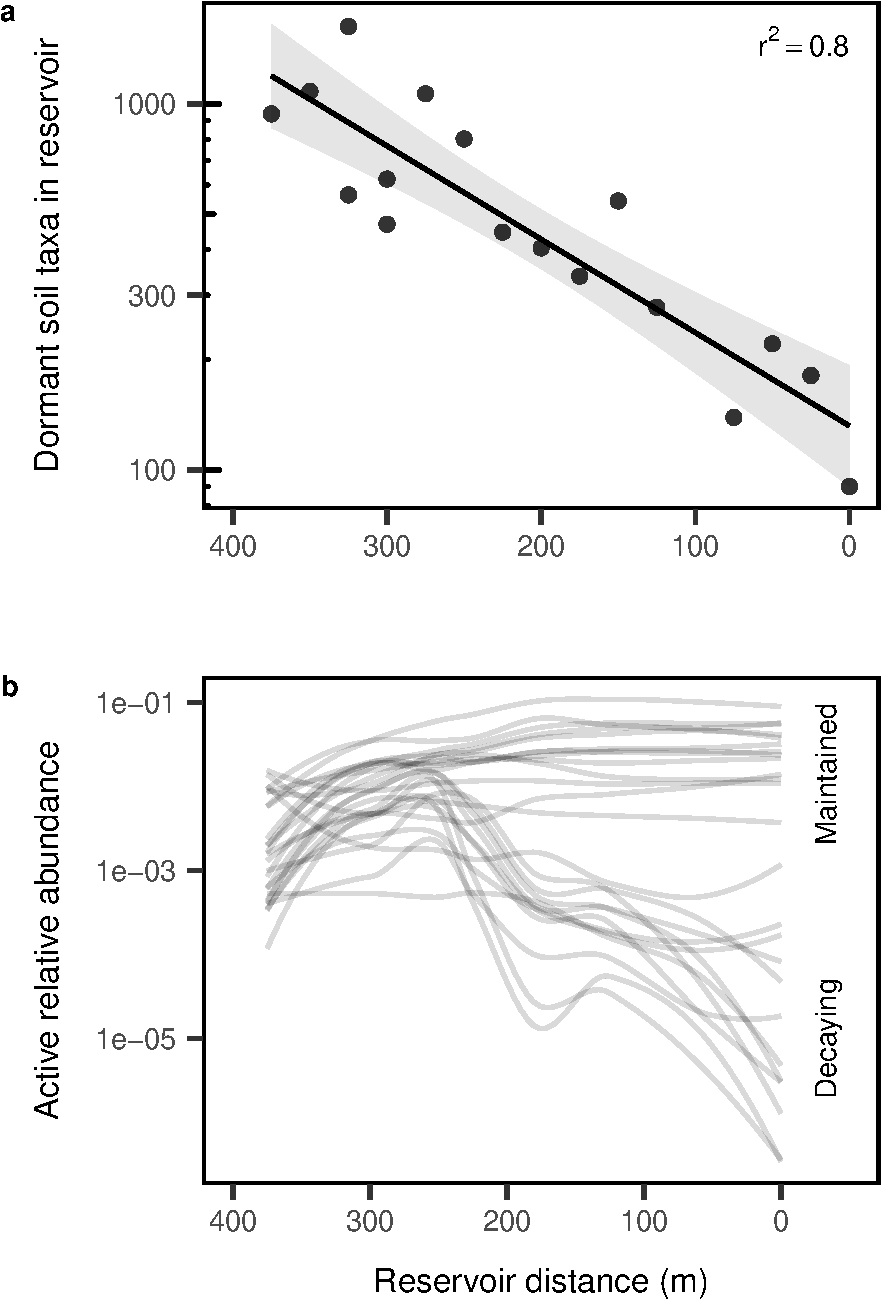
\includegraphics{ReservoirGradient_files/figure-latex/fate_panel-1} \end{center}

\begin{Shaded}
\begin{Highlighting}[]
\CommentTok{# soil.mods <- t(soil.core.mods) %>% as.data.frame()}
\CommentTok{# soil.mods$habitat <- "Present in soils"}
\CommentTok{# soil.mods <- soil.mods %>% rownames_to_column(var = "OTU")}
\CommentTok{# nonsoil.mods <- t(nonsoil.core.mods) %>% as.data.frame()}
\CommentTok{# nonsoil.mods$habitat <- "Absent from soils"}
\CommentTok{# nonsoil.mods <- nonsoil.mods %>% rownames_to_column(var = "OTU")}
\CommentTok{# rbind.data.frame(soil.mods, nonsoil.mods) %>% }
\CommentTok{#   filter(pval < 0.05) %>% }
\CommentTok{#   ggplot(aes(x = -slope, fill = habitat, color = habitat)) +}
\CommentTok{#   geom_line(stat = "density", alpha = 0.5, adjust = .8) +}
\CommentTok{#   geom_density(color = NA, adjust = .8, alpha = 0.2)}
\end{Highlighting}
\end{Shaded}

\section{\texorpdfstring{Are the ``persistent'' reservoir taxa really
representative? Look over
time\ldots{}}{Are the persistent reservoir taxa really representative? Look over time\ldots{}}}\label{are-the-persistent-reservoir-taxa-really-representative-look-over-time}

\begin{Shaded}
\begin{Highlighting}[]
\NormalTok{total.OTUs <-}\StringTok{ }\KeywordTok{read.otu}\NormalTok{(}\DataTypeTok{shared =}\NormalTok{ shared, }\DataTypeTok{cutoff =} \StringTok{"0.03"}\NormalTok{)    }\CommentTok{# 97% Similarity}

\CommentTok{# Import Taxonomy}
\NormalTok{total.OTU.tax <-}\StringTok{ }\KeywordTok{read.tax}\NormalTok{(}\DataTypeTok{taxonomy =}\NormalTok{ taxon, }\DataTypeTok{format =} \StringTok{"rdp"}\NormalTok{)}

\CommentTok{# Subset to just the time series sites}
\NormalTok{UL.ts.OTUs <-}\StringTok{ }\NormalTok{total.OTUs[}\KeywordTok{str_which}\NormalTok{(}\KeywordTok{rownames}\NormalTok{(total.OTUs), }\StringTok{"UL"}\NormalTok{),]}

\CommentTok{# make sure OTU table matches up with design order}
\NormalTok{UL.ts.design <-}\StringTok{ }\KeywordTok{read_csv}\NormalTok{(}\StringTok{"data/UL_timeseries_design.csv"}\NormalTok{)}
\NormalTok{UL.ts.OTUs <-}\StringTok{ }\NormalTok{UL.ts.OTUs[}\KeywordTok{match}\NormalTok{(UL.ts.design}\OperatorTok{$}\NormalTok{sample.name, }\KeywordTok{rownames}\NormalTok{(UL.ts.OTUs)),]}
\NormalTok{UL.ts.OTUs.RNA <-}\StringTok{ }\KeywordTok{decostand}\NormalTok{(UL.ts.OTUs[}\KeywordTok{which}\NormalTok{(UL.ts.design}\OperatorTok{$}\NormalTok{sample.type }\OperatorTok{==}\StringTok{ "RNA"}\NormalTok{),], }\DataTypeTok{method =} \StringTok{"total"}\NormalTok{)}
\NormalTok{UL.ts.OTUs.DNA <-}\StringTok{ }\KeywordTok{decostand}\NormalTok{(UL.ts.OTUs[}\KeywordTok{which}\NormalTok{(UL.ts.design}\OperatorTok{$}\NormalTok{sample.type }\OperatorTok{==}\StringTok{ "DNA"}\NormalTok{),], }\DataTypeTok{method =} \StringTok{"total"}\NormalTok{)}


\NormalTok{env.ts.data <-}\StringTok{ }\KeywordTok{read.table}\NormalTok{(}\StringTok{"data/ul-seedbank.env.txt"}\NormalTok{, }\DataTypeTok{sep=}\StringTok{"}\CharTok{\textbackslash{}t}\StringTok{"}\NormalTok{, }\DataTypeTok{header=}\OtherTok{TRUE}\NormalTok{)}
\NormalTok{env.ts.data}\OperatorTok{$}\NormalTok{date <-}\StringTok{ }\KeywordTok{as.Date}\NormalTok{(}\KeywordTok{parse_date_time}\NormalTok{(env.ts.data}\OperatorTok{$}\NormalTok{date, }\StringTok{"m d y"}\NormalTok{))}
\NormalTok{env.ts.data}\OperatorTok{$}\NormalTok{doc[}\KeywordTok{which}\NormalTok{(env.ts.data}\OperatorTok{$}\NormalTok{doc }\OperatorTok{==}\StringTok{ "**"}\NormalTok{)] <-}\StringTok{ }\OtherTok{NA}
\NormalTok{env.ts.data}\OperatorTok{$}\NormalTok{doc <-}\StringTok{ }\KeywordTok{as.numeric}\NormalTok{(env.ts.data}\OperatorTok{$}\NormalTok{doc)}
\KeywordTok{summary}\NormalTok{(env.ts.data)}
\end{Highlighting}
\end{Shaded}

\begin{verbatim}
##    sample.id           date                 temp            spc        
##  Min.   :  1.00   Min.   :2013-04-19   Min.   : 2.21   Min.   :0.3300  
##  1st Qu.: 31.75   1st Qu.:2013-11-20   1st Qu.: 5.50   1st Qu.:0.4600  
##  Median : 62.50   Median :2014-06-23   Median :17.73   Median :0.5320  
##  Mean   : 62.50   Mean   :2014-06-24   Mean   :16.18   Mean   :0.5172  
##  3rd Qu.: 93.25   3rd Qu.:2015-01-25   3rd Qu.:25.05   3rd Qu.:0.5660  
##  Max.   :124.00   Max.   :2015-09-14   Max.   :29.77   Max.   :0.6700  
##                                        NA's   :2       NA's   :2       
##      oxygen          salinity          secchi            ph        
##  Min.   : 1.870   Min.   :0.1500   Min.   :0.200   Min.   : 6.890  
##  1st Qu.: 5.237   1st Qu.:0.2200   1st Qu.:1.200   1st Qu.: 7.920  
##  Median : 8.355   Median :0.2550   Median :1.600   Median : 8.415  
##  Mean   : 8.961   Mean   :0.2487   Mean   :1.668   Mean   : 8.567  
##  3rd Qu.:10.178   3rd Qu.:0.2700   3rd Qu.:2.200   3rd Qu.: 9.123  
##  Max.   :22.240   Max.   :0.3200   Max.   :3.600   Max.   :10.860  
##  NA's   :2        NA's   :2        NA's   :1       NA's   :2       
##       chla              tp                tn              doc        
##  Min.   :  0.92   Min.   :   8.26   Min.   : 0.407   Min.   :  2.00  
##  1st Qu.: 12.63   1st Qu.:  26.30   1st Qu.: 0.882   1st Qu.: 32.25  
##  Median : 37.67   Median :  34.85   Median : 1.210   Median : 61.50  
##  Mean   : 79.25   Mean   :  84.25   Mean   : 1.889   Mean   : 61.57  
##  3rd Qu.:121.31   3rd Qu.:  47.95   3rd Qu.: 1.490   3rd Qu.: 90.75  
##  Max.   :523.56   Max.   :3200.00   Max.   :42.600   Max.   :121.00  
##  NA's   :2        NA's   :2         NA's   :3        NA's   :2       
##       orp             air.temp     
##  Min.   :-41.800   Min.   :-11.60  
##  1st Qu.:  9.325   1st Qu.:  7.00  
##  Median : 21.700   Median : 18.50  
##  Mean   : 50.507   Mean   : 15.57  
##  3rd Qu.:104.975   3rd Qu.: 24.00  
##  Max.   :225.200   Max.   : 32.00  
##  NA's   :68        NA's   :2
\end{verbatim}

\begin{Shaded}
\begin{Highlighting}[]
\NormalTok{UL.ts.design <-}\StringTok{ }\KeywordTok{left_join}\NormalTok{(UL.ts.design, env.ts.data[,}\KeywordTok{c}\NormalTok{(}\StringTok{"sample.id"}\NormalTok{, }\StringTok{"date"}\NormalTok{)])}
\NormalTok{env.ts.data <-}\StringTok{ }\NormalTok{env.ts.data[}\OperatorTok{-}\KeywordTok{which}\NormalTok{(}\OperatorTok{!}\NormalTok{(env.ts.data}\OperatorTok{$}\NormalTok{date }\OperatorTok\StringTok{ }\NormalTok{UL.ts.design}\OperatorTok{$}\NormalTok{date)),]}

\NormalTok{OTUs.in.core <-}\StringTok{ }\NormalTok{UL.ts.OTUs.RNA[, }\KeywordTok{which}\NormalTok{(}\KeywordTok{colnames}\NormalTok{(UL.ts.OTUs) }\OperatorTok\StringTok{ }\NormalTok{df.plot}\OperatorTok{$}\NormalTok{OTU)]}
\KeywordTok{cbind.data.frame}\NormalTok{(UL.ts.design[}\KeywordTok{which}\NormalTok{(UL.ts.design}\OperatorTok{$}\NormalTok{sample.type }\OperatorTok{==}\StringTok{ "RNA"}\NormalTok{),], OTUs.in.core) }\OperatorTok\StringTok{ }\KeywordTok{as_tibble}\NormalTok{() }\OperatorTok\StringTok{ }
\StringTok{  }\KeywordTok{gather}\NormalTok{(}\OperatorTok{-}\NormalTok{sample.name, }\OperatorTok{-}\NormalTok{sample.type, }\OperatorTok{-}\NormalTok{sample.id, }\OperatorTok{-}\NormalTok{date, }\DataTypeTok{key =}\NormalTok{ OTU, }\DataTypeTok{value =}\NormalTok{ rel_abund) }\OperatorTok\StringTok{ }
\StringTok{  }\KeywordTok{mutate}\NormalTok{(}\DataTypeTok{soils =} \KeywordTok{ifelse}\NormalTok{(OTU }\OperatorTok\StringTok{ }\KeywordTok{unique}\NormalTok{(}\KeywordTok{c}\NormalTok{(df2}\OperatorTok{$}\NormalTok{OTU, df3}\OperatorTok{$}\NormalTok{OTU)), }
                        \StringTok{"Present in soils"}\NormalTok{, }\StringTok{"Absent from soils"}\NormalTok{)) }\OperatorTok\StringTok{ }
\StringTok{  }\KeywordTok{mutate}\NormalTok{(}\DataTypeTok{change =} \KeywordTok{ifelse}\NormalTok{(OTU }\OperatorTok\StringTok{ }\KeywordTok{unique}\NormalTok{(}\KeywordTok{c}\NormalTok{(df3}\OperatorTok{$}\NormalTok{OTU, df4}\OperatorTok{$}\NormalTok{OTU)), }
                        \StringTok{"Decreasing"}\NormalTok{, }\StringTok{"Increasing"}\NormalTok{)) }\OperatorTok\StringTok{ }
\StringTok{  }\KeywordTok{mutate}\NormalTok{(}\DataTypeTok{rel_abund =} \KeywordTok{ifelse}\NormalTok{(rel_abund }\OperatorTok{==}\StringTok{ }\DecValTok{0}\NormalTok{, }\FloatTok{1e-6}\NormalTok{, rel_abund)) }\OperatorTok\StringTok{ }
\StringTok{  }\KeywordTok{ggplot}\NormalTok{(}\KeywordTok{aes}\NormalTok{(}\DataTypeTok{x =}\NormalTok{ date, }\DataTypeTok{y =}\NormalTok{ rel_abund, }\DataTypeTok{group =}\NormalTok{ OTU)) }\OperatorTok{+}
\StringTok{  }\KeywordTok{geom_point}\NormalTok{(}\DataTypeTok{alpha =}\NormalTok{ .}\DecValTok{1}\NormalTok{) }\OperatorTok{+}\StringTok{ }
\StringTok{  }\KeywordTok{geom_line}\NormalTok{(}\DataTypeTok{stat =} \StringTok{"smooth"}\NormalTok{, }\DataTypeTok{method =} \StringTok{"loess"}\NormalTok{, }\DataTypeTok{color =} \StringTok{"blue"}\NormalTok{,}
            \DataTypeTok{alpha =} \FloatTok{0.5}\NormalTok{, }\DataTypeTok{span =}\NormalTok{ .}\DecValTok{5}\NormalTok{, }\DataTypeTok{se =}\NormalTok{ F) }\OperatorTok{+}
\StringTok{  }\KeywordTok{geom_vline}\NormalTok{(}\KeywordTok{aes}\NormalTok{(}\DataTypeTok{xintercept =} \KeywordTok{as_date}\NormalTok{(}\StringTok{"2013-07-15"}\NormalTok{))) }\OperatorTok{+}
\StringTok{  }\KeywordTok{scale_y_log10}\NormalTok{() }\OperatorTok{+}\StringTok{ }
\StringTok{  }\KeywordTok{scale_x_date}\NormalTok{(}\DataTypeTok{labels =}\NormalTok{ scales}\OperatorTok{::}\KeywordTok{date_format}\NormalTok{(}\DataTypeTok{format =} \StringTok{"%b %y"}\NormalTok{)) }\OperatorTok{+}
\StringTok{  }\KeywordTok{theme}\NormalTok{(}\DataTypeTok{axis.text.x =} \KeywordTok{element_text}\NormalTok{(}\DataTypeTok{angle =} \DecValTok{45}\NormalTok{, }\DataTypeTok{hjust =} \DecValTok{1}\NormalTok{)) }\OperatorTok{+}
\StringTok{  }\KeywordTok{facet_grid}\NormalTok{(soils }\OperatorTok{~}\StringTok{ }\NormalTok{change) }\OperatorTok{+}
\StringTok{  }\KeywordTok{labs}\NormalTok{(}\DataTypeTok{x =} \StringTok{""}\NormalTok{,}
       \DataTypeTok{y =} \StringTok{"Relative abundance"}\NormalTok{)}
\end{Highlighting}
\end{Shaded}

\begin{center}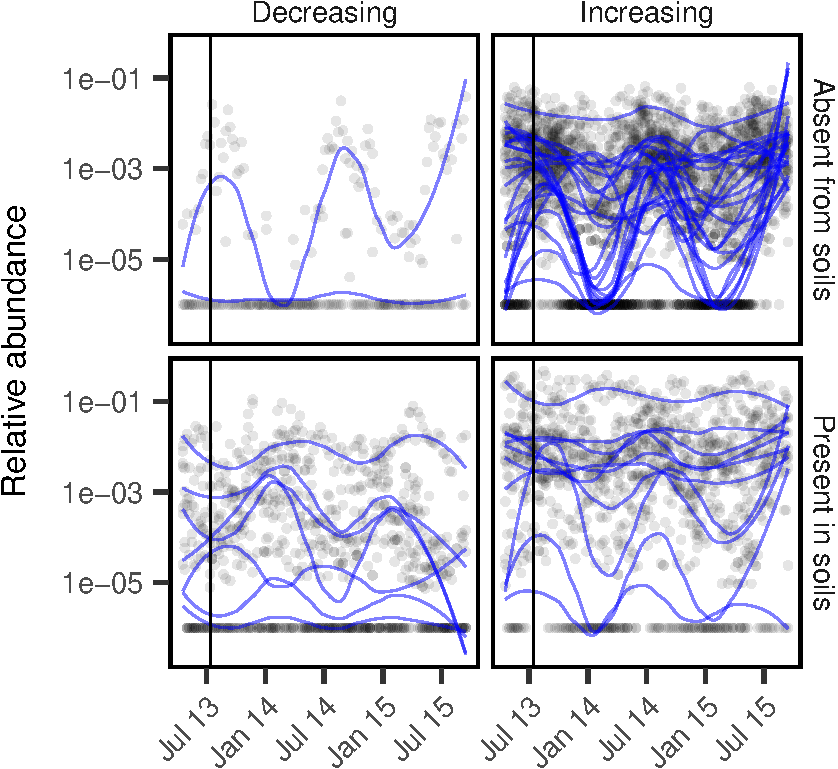
\includegraphics{ReservoirGradient_files/figure-latex/time_series-1} \end{center}

Many of them do appear to track the seasons quite well, suggesting there
could be a seasonality component to the role of terrestrial inputs into
the reservoir.

\section{Not-included}\label{not-included}

\subsection{Ecosystem functions}\label{ecosystem-functions}

\begin{Shaded}
\begin{Highlighting}[]
\NormalTok{metab <-}\StringTok{ }\KeywordTok{read.table}\NormalTok{(}\StringTok{"data/res.grad.metab.txt"}\NormalTok{, }\DataTypeTok{sep=}\StringTok{"}\CharTok{\textbackslash{}t}\StringTok{"}\NormalTok{, }\DataTypeTok{header=}\OtherTok{TRUE}\NormalTok{)}
\KeywordTok{colnames}\NormalTok{(metab) <-}\StringTok{ }\KeywordTok{c}\NormalTok{(}\StringTok{"dist"}\NormalTok{, }\StringTok{"BP"}\NormalTok{, }\StringTok{"BR"}\NormalTok{)}
\NormalTok{BGE <-}\StringTok{ }\KeywordTok{round}\NormalTok{((metab}\OperatorTok{$}\NormalTok{BP}\OperatorTok{/}\NormalTok{(metab}\OperatorTok{$}\NormalTok{BP }\OperatorTok{+}\StringTok{ }\NormalTok{metab}\OperatorTok{$}\NormalTok{BR)),}\DecValTok{3}\NormalTok{)}
\NormalTok{metab <-}\StringTok{ }\KeywordTok{cbind}\NormalTok{(metab, BGE)}


\CommentTok{# Quadratic regression for BP}
\NormalTok{dist <-}\StringTok{ }\NormalTok{metab}\OperatorTok{$}\NormalTok{dist}
\NormalTok{dist2 <-}\StringTok{ }\NormalTok{metab}\OperatorTok{$}\NormalTok{dist}\OperatorTok{^}\DecValTok{2}
\NormalTok{BP.fit <-}\StringTok{ }\KeywordTok{lm}\NormalTok{(metab}\OperatorTok{$}\NormalTok{BP }\OperatorTok{~}\StringTok{ }\NormalTok{dist }\OperatorTok{+}\StringTok{ }\NormalTok{dist2)}
\NormalTok{BP.R2 <-}\StringTok{ }\KeywordTok{round}\NormalTok{(}\KeywordTok{summary}\NormalTok{(BP.fit)}\OperatorTok{$}\NormalTok{r.squared, }\DecValTok{2}\NormalTok{)}

\CommentTok{# Simple linear regression for BR}
\NormalTok{BR.fit <-}\StringTok{ }\KeywordTok{lm}\NormalTok{(metab}\OperatorTok{$}\NormalTok{BR }\OperatorTok{~}\StringTok{ }\NormalTok{metab}\OperatorTok{$}\NormalTok{dist)}
\NormalTok{BR.R2 <-}\StringTok{ }\KeywordTok{round}\NormalTok{(}\KeywordTok{summary}\NormalTok{(BR.fit)}\OperatorTok{$}\NormalTok{r.squared, }\DecValTok{2}\NormalTok{)}
\NormalTok{BR.int <-}\StringTok{ }\NormalTok{BR.fit}\OperatorTok{$}\NormalTok{coefficients[}\DecValTok{1}\NormalTok{]}
\NormalTok{BR.slp <-}\StringTok{ }\NormalTok{BR.fit}\OperatorTok{$}\NormalTok{coefficients[}\DecValTok{2}\NormalTok{]}

\CommentTok{# Simple linear regression for BGE}
\NormalTok{BGE.fit <-}\StringTok{ }\KeywordTok{lm}\NormalTok{(metab}\OperatorTok{$}\NormalTok{BGE }\OperatorTok{~}\StringTok{ }\NormalTok{metab}\OperatorTok{$}\NormalTok{dist)}
\NormalTok{BGE.R2 <-}\StringTok{ }\KeywordTok{round}\NormalTok{(}\KeywordTok{summary}\NormalTok{(BGE.fit)}\OperatorTok{$}\NormalTok{r.squared, }\DecValTok{2}\NormalTok{)}
\NormalTok{BGE.int <-}\StringTok{ }\NormalTok{BGE.fit}\OperatorTok{$}\NormalTok{coefficients[}\DecValTok{1}\NormalTok{]}
\NormalTok{BGE.slp <-}\StringTok{ }\NormalTok{BGE.fit}\OperatorTok{$}\NormalTok{coefficients[}\DecValTok{2}\NormalTok{]}

\NormalTok{BP.R2}
\NormalTok{BR.R2}
\NormalTok{BGE.R2}

\NormalTok{BP.plot <-}\StringTok{ }\KeywordTok{ggplot}\NormalTok{(metab, }\KeywordTok{aes}\NormalTok{(}\DataTypeTok{x =}\NormalTok{ dist, }\DataTypeTok{y =}\NormalTok{ BP)) }\OperatorTok{+}\StringTok{ }
\StringTok{  }\KeywordTok{geom_point}\NormalTok{() }\OperatorTok{+}\StringTok{ }
\StringTok{  }\KeywordTok{geom_smooth}\NormalTok{(}\DataTypeTok{method =} \StringTok{"lm"}\NormalTok{, }\DataTypeTok{formula =}\NormalTok{ y }\OperatorTok{~}\StringTok{ }\NormalTok{x }\OperatorTok{+}\StringTok{ }\KeywordTok{I}\NormalTok{(x}\OperatorTok{^}\DecValTok{2}\NormalTok{), }\DataTypeTok{color =} \StringTok{"black"}\NormalTok{) }\OperatorTok{+}
\StringTok{  }\KeywordTok{annotate}\NormalTok{(}\DataTypeTok{geom =} \StringTok{"text"}\NormalTok{, }\DataTypeTok{x =} \DecValTok{50}\NormalTok{, }\DataTypeTok{y =} \FloatTok{1.5}\NormalTok{, }\DataTypeTok{size =} \DecValTok{5}\NormalTok{, }
           \DataTypeTok{label =} \KeywordTok{paste0}\NormalTok{(}\StringTok{"R^2== "}\NormalTok{,BP.R2), }\DataTypeTok{parse =}\NormalTok{ T) }\OperatorTok{+}
\StringTok{  }\KeywordTok{labs}\NormalTok{(}\DataTypeTok{y =} \KeywordTok{expression}\NormalTok{(}\KeywordTok{paste}\NormalTok{(}\StringTok{'BP ('}\NormalTok{, mu ,}\StringTok{'M C h'}\OperatorTok{^-}\DecValTok{1}\OperatorTok{*}\StringTok{ ')'}\NormalTok{)), }
       \DataTypeTok{x =} \StringTok{"Reservoir Transect (m)"}\NormalTok{) }\OperatorTok{+}
\StringTok{  }\KeywordTok{scale_x_reverse}\NormalTok{(}\DataTypeTok{limits =} \KeywordTok{c}\NormalTok{(}\DecValTok{400}\NormalTok{,}\DecValTok{0}\NormalTok{))}
\NormalTok{BR.plot <-}\StringTok{ }\KeywordTok{ggplot}\NormalTok{(metab, }\KeywordTok{aes}\NormalTok{(}\DataTypeTok{x =}\NormalTok{ dist, }\DataTypeTok{y =}\NormalTok{ BR)) }\OperatorTok{+}\StringTok{ }
\StringTok{  }\KeywordTok{geom_point}\NormalTok{() }\OperatorTok{+}\StringTok{ }
\StringTok{  }\KeywordTok{geom_smooth}\NormalTok{(}\DataTypeTok{method =} \StringTok{"lm"}\NormalTok{, }\DataTypeTok{formula =}\NormalTok{ y }\OperatorTok{~}\StringTok{ }\NormalTok{x, }\DataTypeTok{color =} \StringTok{"black"}\NormalTok{) }\OperatorTok{+}\StringTok{ }
\StringTok{  }\KeywordTok{annotate}\NormalTok{(}\StringTok{"text"}\NormalTok{, }\DataTypeTok{x =} \DecValTok{50}\NormalTok{, }\DataTypeTok{y =} \FloatTok{1.5}\NormalTok{, }\DataTypeTok{size =} \DecValTok{5}\NormalTok{, }
           \DataTypeTok{label =} \KeywordTok{paste0}\NormalTok{(}\StringTok{"R^2== "}\NormalTok{,BR.R2), }\DataTypeTok{parse =}\NormalTok{ T ) }\OperatorTok{+}
\StringTok{  }\KeywordTok{labs}\NormalTok{(}\DataTypeTok{y =} \KeywordTok{expression}\NormalTok{(}\KeywordTok{paste}\NormalTok{(}\StringTok{'BR ('}\NormalTok{, mu ,}\StringTok{'M C h'}\OperatorTok{^-}\DecValTok{1}\OperatorTok{*}\StringTok{ ')'}\NormalTok{)), }
       \DataTypeTok{x =} \StringTok{"Reservoir Transect (m)"}\NormalTok{) }\OperatorTok{+}
\StringTok{  }\KeywordTok{scale_x_reverse}\NormalTok{(}\DataTypeTok{limits =} \KeywordTok{c}\NormalTok{(}\DecValTok{400}\NormalTok{,}\DecValTok{0}\NormalTok{))}
\NormalTok{BGE.plot <-}\StringTok{ }\KeywordTok{ggplot}\NormalTok{(metab, }\KeywordTok{aes}\NormalTok{(}\DataTypeTok{x =}\NormalTok{ dist, }\DataTypeTok{y =}\NormalTok{ BGE)) }\OperatorTok{+}\StringTok{ }
\StringTok{  }\KeywordTok{geom_point}\NormalTok{() }\OperatorTok{+}\StringTok{ }
\StringTok{  }\KeywordTok{geom_smooth}\NormalTok{(}\DataTypeTok{method =} \StringTok{"lm"}\NormalTok{, }\DataTypeTok{formula =}\NormalTok{ y }\OperatorTok{~}\StringTok{ }\NormalTok{x }\OperatorTok{+}\StringTok{ }\KeywordTok{I}\NormalTok{(x}\OperatorTok{^}\DecValTok{2}\NormalTok{), }\DataTypeTok{color =} \StringTok{"black"}\NormalTok{) }\OperatorTok{+}
\StringTok{  }\KeywordTok{annotate}\NormalTok{(}\StringTok{"text"}\NormalTok{, }\DataTypeTok{x =} \DecValTok{50}\NormalTok{, }\DataTypeTok{y =}\NormalTok{ .}\DecValTok{5}\NormalTok{, }\DataTypeTok{size =} \DecValTok{5}\NormalTok{, }
           \DataTypeTok{label =} \KeywordTok{paste0}\NormalTok{(}\StringTok{"R^2== "}\NormalTok{,BGE.R2), }\DataTypeTok{parse =}\NormalTok{ T ) }\OperatorTok{+}
\StringTok{  }\KeywordTok{labs}\NormalTok{(}\DataTypeTok{y =} \StringTok{"BGE"}\NormalTok{, }
       \DataTypeTok{x =} \StringTok{"Reservoir Transect (m)"}\NormalTok{) }\OperatorTok{+}
\StringTok{  }\KeywordTok{scale_x_reverse}\NormalTok{(}\DataTypeTok{limits =} \KeywordTok{c}\NormalTok{(}\DecValTok{400}\NormalTok{,}\DecValTok{0}\NormalTok{))}
\end{Highlighting}
\end{Shaded}

\begin{Shaded}
\begin{Highlighting}[]
\KeywordTok{plot_grid}\NormalTok{(BP.plot }\OperatorTok{+}\StringTok{ }\KeywordTok{theme}\NormalTok{(}\DataTypeTok{axis.title.x =} \KeywordTok{element_blank}\NormalTok{(), }\DataTypeTok{axis.text.x =} \KeywordTok{element_blank}\NormalTok{(), }
                          \DataTypeTok{plot.margin =} \KeywordTok{unit}\NormalTok{(}\KeywordTok{c}\NormalTok{(}\DecValTok{1}\NormalTok{, }\DecValTok{1}\NormalTok{, }\OperatorTok{-}\DecValTok{1}\NormalTok{, }\DecValTok{0}\NormalTok{), }\StringTok{"cm"}\NormalTok{)), }
\NormalTok{          BR.plot }\OperatorTok{+}\StringTok{ }\KeywordTok{theme}\NormalTok{(}\DataTypeTok{axis.title.x =} \KeywordTok{element_blank}\NormalTok{(), }\DataTypeTok{axis.text.x =} \KeywordTok{element_blank}\NormalTok{(),}
                          \DataTypeTok{plot.margin =} \KeywordTok{unit}\NormalTok{(}\KeywordTok{c}\NormalTok{(}\OperatorTok{-}\DecValTok{1}\NormalTok{, }\DecValTok{1}\NormalTok{, }\OperatorTok{-}\DecValTok{1}\NormalTok{, }\DecValTok{0}\NormalTok{), }\StringTok{"cm"}\NormalTok{)), }
\NormalTok{          BGE.plot }\OperatorTok{+}\StringTok{ }\KeywordTok{theme}\NormalTok{(}\DataTypeTok{plot.margin =} \KeywordTok{unit}\NormalTok{(}\KeywordTok{c}\NormalTok{(}\OperatorTok{-}\DecValTok{1}\NormalTok{, }\DecValTok{1}\NormalTok{, }\DecValTok{0}\NormalTok{, }\DecValTok{0}\NormalTok{), }\StringTok{"cm"}\NormalTok{)), }
          \DataTypeTok{align =} \StringTok{"hv"}\NormalTok{, }\DataTypeTok{ncol =} \DecValTok{1}\NormalTok{, }\DataTypeTok{labels =} \StringTok{"AUTO"}\NormalTok{)}
\end{Highlighting}
\end{Shaded}

\begin{center}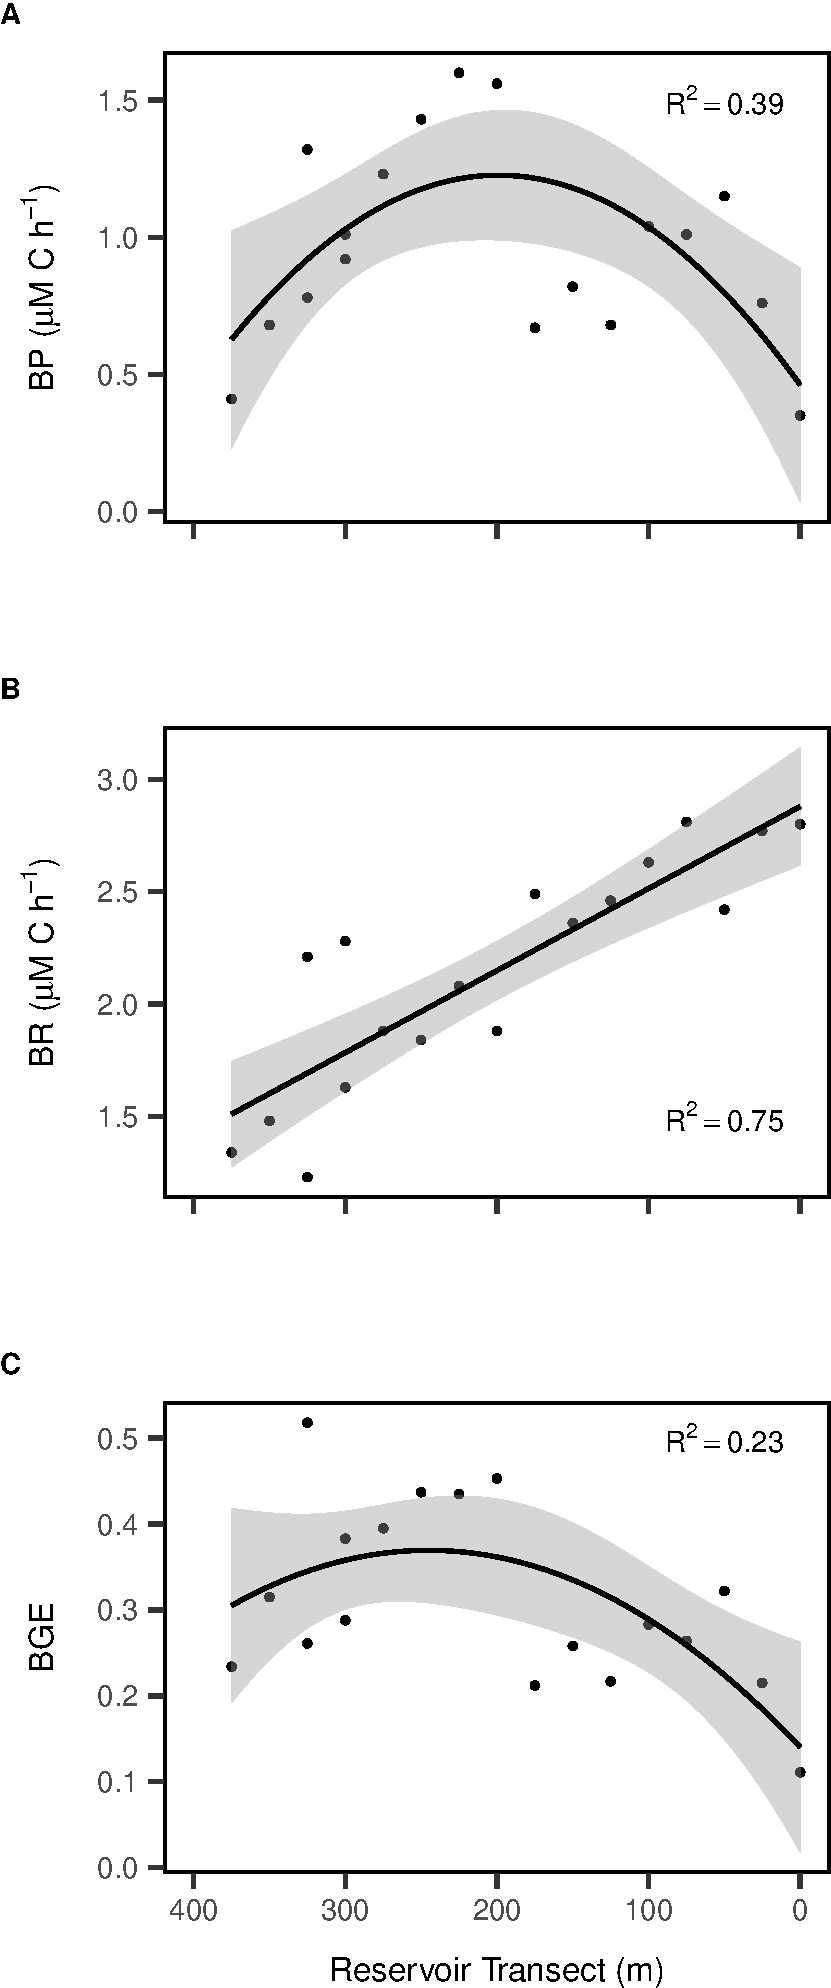
\includegraphics{ReservoirGradient_files/figure-latex/metab_plot-1} \end{center}

\subsection{Relation of ecosystem functions and community
structure}\label{relation-of-ecosystem-functions-and-community-structure}

\begin{Shaded}
\begin{Highlighting}[]
\CommentTok{# detrend the spatial signal}
\NormalTok{bp.resid <-}\StringTok{ }\KeywordTok{resid}\NormalTok{(}\KeywordTok{lm}\NormalTok{(BP }\OperatorTok{~}\StringTok{ }\NormalTok{dist }\OperatorTok{+}\StringTok{ }\KeywordTok{I}\NormalTok{(dist)}\OperatorTok{^}\DecValTok{2}\NormalTok{, }\DataTypeTok{data =}\NormalTok{ metab))}
\NormalTok{br.resid <-}\StringTok{ }\KeywordTok{resid}\NormalTok{(}\KeywordTok{lm}\NormalTok{(BR }\OperatorTok{~}\StringTok{ }\NormalTok{dist, }\DataTypeTok{data =}\NormalTok{ metab))}


\NormalTok{metab.resids <-}\StringTok{ }\NormalTok{metab}
\NormalTok{metab.resids}\OperatorTok{$}\NormalTok{BR_resid <-}\StringTok{ }\NormalTok{br.resid }\OperatorTok{+}\StringTok{ }\KeywordTok{mean}\NormalTok{(metab}\OperatorTok{$}\NormalTok{BR)}
\NormalTok{metab.resids}\OperatorTok{$}\NormalTok{BP_resid <-}\StringTok{ }\NormalTok{bp.resid }\OperatorTok{+}\StringTok{ }\KeywordTok{mean}\NormalTok{(metab}\OperatorTok{$}\NormalTok{BP)}

\NormalTok{transient.metabolism <-}\StringTok{ }\KeywordTok{data.frame}\NormalTok{(}\DataTypeTok{transients =}\NormalTok{ terr.REL, }\DataTypeTok{dist =}\NormalTok{ design.dna}\OperatorTok{$}\NormalTok{distance) }\OperatorTok\StringTok{ }
\StringTok{  }\KeywordTok{left_join}\NormalTok{(metab.resids) }


\NormalTok{bp.mod.quad <-}\StringTok{ }\KeywordTok{lm}\NormalTok{(BP_resid }\OperatorTok{~}\StringTok{ }\NormalTok{transients }\OperatorTok{+}\StringTok{ }\KeywordTok{I}\NormalTok{(transients}\OperatorTok{^}\DecValTok{2}\NormalTok{), }\DataTypeTok{data =}\NormalTok{ transient.metabolism)}
\NormalTok{bp.mod.lin <-}\StringTok{ }\KeywordTok{lm}\NormalTok{(BP_resid }\OperatorTok{~}\StringTok{ }\NormalTok{transients, }\DataTypeTok{data =}\NormalTok{ transient.metabolism)}
\NormalTok{bp.mod.int <-}\StringTok{ }\KeywordTok{lm}\NormalTok{(BP_resid }\OperatorTok{~}\StringTok{ }\DecValTok{1}\NormalTok{, }\DataTypeTok{data =}\NormalTok{ transient.metabolism)}
\KeywordTok{anova}\NormalTok{(bp.mod.int, bp.mod.lin, bp.mod.quad)}
\KeywordTok{AIC}\NormalTok{(bp.mod.quad, bp.mod.lin, bp.mod.int)}

\NormalTok{br.mod.quad <-}\StringTok{ }\KeywordTok{lm}\NormalTok{(BR_resid }\OperatorTok{~}\StringTok{ }\NormalTok{transients }\OperatorTok{+}\StringTok{ }\KeywordTok{I}\NormalTok{(transients}\OperatorTok{^}\DecValTok{2}\NormalTok{), }\DataTypeTok{data =}\NormalTok{ transient.metabolism)}
\NormalTok{br.mod.lin <-}\StringTok{ }\KeywordTok{lm}\NormalTok{(BR_resid }\OperatorTok{~}\StringTok{ }\NormalTok{transients, }\DataTypeTok{data =}\NormalTok{ transient.metabolism)}
\NormalTok{br.mod.int <-}\StringTok{ }\KeywordTok{lm}\NormalTok{(BR_resid }\OperatorTok{~}\StringTok{ }\DecValTok{1}\NormalTok{, }\DataTypeTok{data =}\NormalTok{ transient.metabolism)}
\KeywordTok{anova}\NormalTok{(br.mod.int, br.mod.lin, br.mod.quad)}
\KeywordTok{AIC}\NormalTok{(br.mod.int, br.mod.lin, br.mod.quad)}

\NormalTok{bge.mod.quad <-}\StringTok{ }\KeywordTok{lm}\NormalTok{(BGE }\OperatorTok{~}\StringTok{ }\NormalTok{transients }\OperatorTok{+}\StringTok{ }\KeywordTok{I}\NormalTok{(transients}\OperatorTok{^}\DecValTok{2}\NormalTok{), }\DataTypeTok{data =}\NormalTok{ transient.metabolism)}
\NormalTok{bge.mod.lin <-}\StringTok{ }\KeywordTok{lm}\NormalTok{(BGE }\OperatorTok{~}\StringTok{ }\NormalTok{transients, }\DataTypeTok{data =}\NormalTok{ transient.metabolism)}
\NormalTok{bge.mod.int <-}\StringTok{ }\KeywordTok{lm}\NormalTok{(BGE }\OperatorTok{~}\StringTok{ }\DecValTok{1}\NormalTok{, }\DataTypeTok{data =}\NormalTok{ transient.metabolism)}
\KeywordTok{anova}\NormalTok{(bge.mod.int, bge.mod.lin, bge.mod.quad)}
\KeywordTok{AIC}\NormalTok{(bge.mod.int, bge.mod.lin, bge.mod.quad)}

\KeywordTok{round}\NormalTok{(}\KeywordTok{summary}\NormalTok{(br.mod.quad)}\OperatorTok{$}\NormalTok{r.squared, }\DecValTok{2}\NormalTok{)}
\KeywordTok{round}\NormalTok{(}\KeywordTok{summary}\NormalTok{(bp.mod.quad)}\OperatorTok{$}\NormalTok{r.squared, }\DecValTok{2}\NormalTok{)}


\NormalTok{total_core <-}\StringTok{ }\KeywordTok{rowSums}\NormalTok{(OTUsREL[design}\OperatorTok{$}\NormalTok{molecule }\OperatorTok{==}\StringTok{ "DNA"} \OperatorTok{&}\StringTok{ }\NormalTok{design}\OperatorTok{$}\NormalTok{type }\OperatorTok{==}\StringTok{ "water"}\NormalTok{,}
                               \KeywordTok{subset}\NormalTok{(}\KeywordTok{rbind.data.frame}\NormalTok{(high.activity.water.core, }
\NormalTok{                                                       high.activity.soil.core), RNA.max }\OperatorTok{>}\StringTok{ }\NormalTok{.}\DecValTok{01}\NormalTok{)}\OperatorTok{$}\NormalTok{OTU])}

\KeywordTok{summary}\NormalTok{(}\KeywordTok{lm}\NormalTok{(BP }\OperatorTok{~}\StringTok{ }\NormalTok{transients }\OperatorTok{*}\StringTok{ }\NormalTok{dist, transient.metabolism))}
\KeywordTok{summary}\NormalTok{(}\KeywordTok{lm}\NormalTok{(BR }\OperatorTok{~}\StringTok{ }\NormalTok{transients }\OperatorTok{*}\StringTok{ }\NormalTok{dist, transient.metabolism))}


\KeywordTok{data.frame}\NormalTok{(}
  \DataTypeTok{soil_core =} \KeywordTok{rowSums}\NormalTok{(OTUsREL[design}\OperatorTok{$}\NormalTok{molecule }\OperatorTok{==}\StringTok{ "DNA"} \OperatorTok{&}\StringTok{ }\NormalTok{design}\OperatorTok{$}\NormalTok{type }\OperatorTok{==}\StringTok{ "water"}\NormalTok{,}
           \KeywordTok{subset}\NormalTok{(soil.vs.lake.abunds, RNA.max }\OperatorTok{>}\StringTok{ }\NormalTok{.}\DecValTok{01}\NormalTok{)}\OperatorTok{$}\NormalTok{OTU]), }
  \DataTypeTok{dist =}\NormalTok{ design.dna}\OperatorTok{$}\NormalTok{distance) }\OperatorTok\StringTok{ }
\StringTok{  }\KeywordTok{left_join}\NormalTok{(metab.resids) }\OperatorTok\StringTok{ }\KeywordTok{select}\NormalTok{(}\OperatorTok{-}\NormalTok{BGE, }\OperatorTok{-}\NormalTok{BP, }\OperatorTok{-}\NormalTok{BR) }\OperatorTok\StringTok{ }\KeywordTok{gather}\NormalTok{(metab, value, }\OperatorTok{-}\NormalTok{soil_core, }\OperatorTok{-}\NormalTok{dist) }\OperatorTok\StringTok{ }
\StringTok{  }\KeywordTok{ggplot}\NormalTok{(}\KeywordTok{aes}\NormalTok{(}\DataTypeTok{x =}\NormalTok{ soil_core, }\DataTypeTok{y =}\NormalTok{ value, }\DataTypeTok{color =}\NormalTok{ metab, }\DataTypeTok{fill =}\NormalTok{ metab)) }\OperatorTok{+}
\StringTok{  }\KeywordTok{geom_point}\NormalTok{(}\DataTypeTok{size =} \DecValTok{2}\NormalTok{) }\OperatorTok{+}\StringTok{ }
\StringTok{  }\KeywordTok{geom_smooth}\NormalTok{(}\DataTypeTok{alpha =}\NormalTok{ .}\DecValTok{25}\NormalTok{, }\DataTypeTok{method =} \StringTok{'lm'}\NormalTok{, }\DataTypeTok{formula =}\NormalTok{ y }\OperatorTok{~}\StringTok{ }\NormalTok{x }\OperatorTok{+}\StringTok{ }\KeywordTok{I}\NormalTok{(x}\OperatorTok{^}\DecValTok{2}\NormalTok{)) }\OperatorTok{+}
\StringTok{  }\KeywordTok{labs}\NormalTok{(}\DataTypeTok{x =} \StringTok{"Relative Abundance of Soil-derived Core"}\NormalTok{,}
       \DataTypeTok{y =} \KeywordTok{expression}\NormalTok{(}\KeywordTok{paste}\NormalTok{(}\StringTok{'Metabolism ('}\NormalTok{, mu ,}\StringTok{'M C h'}\OperatorTok{^-}\DecValTok{1}\OperatorTok{*}\StringTok{ ')'}\NormalTok{))) }\OperatorTok{+}
\StringTok{  }\KeywordTok{scale_color_viridis}\NormalTok{(}\StringTok{"Ecosystem Function"}\NormalTok{, }\DataTypeTok{discrete =}\NormalTok{ T, }\DataTypeTok{begin =}\NormalTok{ .}\DecValTok{1}\NormalTok{, }\DataTypeTok{end =}\NormalTok{ .}\DecValTok{6}\NormalTok{, }\DataTypeTok{option =} \StringTok{"D"}\NormalTok{) }\OperatorTok{+}
\StringTok{  }\KeywordTok{scale_fill_viridis}\NormalTok{(}\StringTok{"Ecosystem Function"}\NormalTok{, }\DataTypeTok{discrete =}\NormalTok{ T, }\DataTypeTok{begin =}\NormalTok{ .}\DecValTok{1}\NormalTok{, }\DataTypeTok{end =}\NormalTok{ .}\DecValTok{6}\NormalTok{, }\DataTypeTok{option =} \StringTok{"D"}\NormalTok{) }\OperatorTok{+}
\StringTok{  }\KeywordTok{ggsave}\NormalTok{(}\StringTok{"figures/06_soilcore-function.pdf"}\NormalTok{, }\DataTypeTok{bg =} \StringTok{"white"}\NormalTok{, }\DataTypeTok{width =} \DecValTok{7}\NormalTok{, }\DataTypeTok{height =} \DecValTok{6}\NormalTok{)}

\KeywordTok{data.frame}\NormalTok{(}
  \DataTypeTok{water_core =} \KeywordTok{rowSums}\NormalTok{(OTUsREL[design}\OperatorTok{$}\NormalTok{molecule }\OperatorTok{==}\StringTok{ "DNA"} \OperatorTok{&}\StringTok{ }\NormalTok{design}\OperatorTok{$}\NormalTok{type }\OperatorTok{==}\StringTok{ "water"}\NormalTok{,}
                               \KeywordTok{subset}\NormalTok{(high.activity.water.core, RNA.max }\OperatorTok{>}\StringTok{ }\NormalTok{.}\DecValTok{01}\NormalTok{)}\OperatorTok{$}\NormalTok{OTU]), }
  \DataTypeTok{dist =}\NormalTok{ design.dna}\OperatorTok{$}\NormalTok{distance) }\OperatorTok\StringTok{ }
\StringTok{  }\KeywordTok{left_join}\NormalTok{(metab.resids) }\OperatorTok\StringTok{ }\KeywordTok{select}\NormalTok{(}\OperatorTok{-}\NormalTok{BGE,}\OperatorTok{-}\NormalTok{BR,}\OperatorTok{-}\NormalTok{BP) }\OperatorTok\StringTok{ }\KeywordTok{gather}\NormalTok{(metab, value, }\OperatorTok{-}\NormalTok{water_core, }\OperatorTok{-}\NormalTok{dist) }\OperatorTok\StringTok{ }
\StringTok{  }\KeywordTok{ggplot}\NormalTok{(}\KeywordTok{aes}\NormalTok{(}\DataTypeTok{x =}\NormalTok{ water_core, }\DataTypeTok{y =}\NormalTok{ value, }\DataTypeTok{color =}\NormalTok{ metab, }\DataTypeTok{fill =}\NormalTok{ metab)) }\OperatorTok{+}
\StringTok{  }\KeywordTok{geom_point}\NormalTok{(}\DataTypeTok{size =} \DecValTok{2}\NormalTok{) }\OperatorTok{+}\StringTok{ }
\StringTok{  }\KeywordTok{geom_smooth}\NormalTok{(}\DataTypeTok{alpha =}\NormalTok{ .}\DecValTok{25}\NormalTok{, }\DataTypeTok{method =} \StringTok{'lm'}\NormalTok{, }\DataTypeTok{formula =}\NormalTok{ y }\OperatorTok{~}\StringTok{ }\NormalTok{x }\OperatorTok{+}\StringTok{ }\KeywordTok{I}\NormalTok{(x}\OperatorTok{^}\DecValTok{2}\NormalTok{)) }\OperatorTok{+}
\StringTok{  }\KeywordTok{labs}\NormalTok{(}\DataTypeTok{x =} \StringTok{"Relative Abundance of non-soil-derived Core"}\NormalTok{,}
       \DataTypeTok{y =} \KeywordTok{expression}\NormalTok{(}\KeywordTok{paste}\NormalTok{(}\StringTok{'Metabolism ('}\NormalTok{, mu ,}\StringTok{'M C h'}\OperatorTok{^-}\DecValTok{1}\OperatorTok{*}\StringTok{ ')'}\NormalTok{))) }\OperatorTok{+}
\StringTok{  }\KeywordTok{scale_color_viridis}\NormalTok{(}\StringTok{"Ecosystem Function"}\NormalTok{, }\DataTypeTok{discrete =}\NormalTok{ T, }\DataTypeTok{begin =}\NormalTok{ .}\DecValTok{1}\NormalTok{, }\DataTypeTok{end =}\NormalTok{ .}\DecValTok{6}\NormalTok{, }\DataTypeTok{option =} \StringTok{"D"}\NormalTok{) }\OperatorTok{+}
\StringTok{  }\KeywordTok{scale_fill_viridis}\NormalTok{(}\StringTok{"Ecosystem Function"}\NormalTok{, }\DataTypeTok{discrete =}\NormalTok{ T, }\DataTypeTok{begin =}\NormalTok{ .}\DecValTok{1}\NormalTok{, }\DataTypeTok{end =}\NormalTok{ .}\DecValTok{6}\NormalTok{, }\DataTypeTok{option =} \StringTok{"D"}\NormalTok{) }\OperatorTok{+}
\StringTok{  }\KeywordTok{ggsave}\NormalTok{(}\StringTok{"figures/06_nonsoilcore-function.pdf"}\NormalTok{, }\DataTypeTok{bg =} \StringTok{"white"}\NormalTok{, }\DataTypeTok{width =} \DecValTok{7}\NormalTok{, }\DataTypeTok{height =} \DecValTok{6}\NormalTok{)}



\KeywordTok{data.frame}\NormalTok{(}\DataTypeTok{transients =} \KeywordTok{resid}\NormalTok{(}\KeywordTok{lm}\NormalTok{(terr.REL }\OperatorTok{~}\StringTok{ }\NormalTok{design.dna}\OperatorTok{$}\NormalTok{distance)) }\OperatorTok{+}\StringTok{ }\KeywordTok{mean}\NormalTok{(terr.REL), }\DataTypeTok{dist =}\NormalTok{ design.dna}\OperatorTok{$}\NormalTok{distance) }\OperatorTok\StringTok{ }
\StringTok{  }\KeywordTok{left_join}\NormalTok{(metab.resids) }\OperatorTok\StringTok{ }\KeywordTok{select}\NormalTok{(}\OperatorTok{-}\NormalTok{BGE, }\OperatorTok{-}\NormalTok{BP, }\OperatorTok{-}\NormalTok{BR) }\OperatorTok\StringTok{ }\KeywordTok{gather}\NormalTok{(metab, value, }\OperatorTok{-}\NormalTok{transients, }\OperatorTok{-}\NormalTok{dist) }\OperatorTok\StringTok{ }
\StringTok{  }\KeywordTok{ggplot}\NormalTok{(}\KeywordTok{aes}\NormalTok{(}\DataTypeTok{x =}\NormalTok{ transients, }\DataTypeTok{y =}\NormalTok{ value, }\DataTypeTok{color =}\NormalTok{ metab, }\DataTypeTok{fill =}\NormalTok{ metab)) }\OperatorTok{+}
\StringTok{  }\KeywordTok{geom_point}\NormalTok{(}\DataTypeTok{size =} \DecValTok{2}\NormalTok{, }\DataTypeTok{show.legend =}\NormalTok{ F) }\OperatorTok{+}\StringTok{ }
\StringTok{  }\KeywordTok{geom_smooth}\NormalTok{(}\DataTypeTok{alpha =}\NormalTok{ .}\DecValTok{25}\NormalTok{, }\DataTypeTok{method =} \StringTok{'lm'}\NormalTok{, }\DataTypeTok{formula =}\NormalTok{ y }\OperatorTok{~}\StringTok{ }\NormalTok{x, }\DataTypeTok{show.legend =}\NormalTok{ F) }\OperatorTok{+}
\StringTok{  }\KeywordTok{annotation_logticks}\NormalTok{(}\DataTypeTok{sides =} \StringTok{"b"}\NormalTok{) }\OperatorTok{+}
\StringTok{  }\KeywordTok{labs}\NormalTok{(}\DataTypeTok{x =} \StringTok{"Relative Abundance of Transient Taxa"}\NormalTok{,}
       \DataTypeTok{y =} \KeywordTok{expression}\NormalTok{(}\KeywordTok{paste}\NormalTok{(}\StringTok{'Metabolism ('}\NormalTok{, mu ,}\StringTok{'M C h'}\OperatorTok{^-}\DecValTok{1}\OperatorTok{*}\StringTok{ ')'}\NormalTok{))) }\OperatorTok{+}
\StringTok{  }\KeywordTok{scale_color_viridis}\NormalTok{(}\StringTok{"Ecosystem Function"}\NormalTok{, }\DataTypeTok{discrete =}\NormalTok{ T, }\DataTypeTok{begin =}\NormalTok{ .}\DecValTok{1}\NormalTok{, }\DataTypeTok{end =}\NormalTok{ .}\DecValTok{6}\NormalTok{, }\DataTypeTok{option =} \StringTok{"D"}\NormalTok{) }\OperatorTok{+}
\StringTok{  }\KeywordTok{scale_fill_viridis}\NormalTok{(}\StringTok{"Ecosystem Function"}\NormalTok{, }\DataTypeTok{discrete =}\NormalTok{ T, }\DataTypeTok{begin =}\NormalTok{ .}\DecValTok{1}\NormalTok{, }\DataTypeTok{end =}\NormalTok{ .}\DecValTok{6}\NormalTok{, }\DataTypeTok{option =} \StringTok{"D"}\NormalTok{) }\OperatorTok{+}
\StringTok{  }\KeywordTok{scale_y_continuous}\NormalTok{(}\DataTypeTok{limits =} \KeywordTok{c}\NormalTok{(}\DecValTok{0}\NormalTok{,}\DecValTok{3}\NormalTok{)) }\OperatorTok{+}
\StringTok{  }\KeywordTok{theme}\NormalTok{(}\DataTypeTok{plot.margin =} \KeywordTok{unit}\NormalTok{(}\KeywordTok{c}\NormalTok{(}\DecValTok{1}\NormalTok{,}\DecValTok{1}\NormalTok{,}\DecValTok{0}\NormalTok{,}\DecValTok{0}\NormalTok{), }\StringTok{"cm"}\NormalTok{)) }\OperatorTok{+}
\StringTok{  }\KeywordTok{ggsave}\NormalTok{(}\StringTok{"figures/06_transients-function.pdf"}\NormalTok{, }\DataTypeTok{bg =} \StringTok{"white"}\NormalTok{, }\DataTypeTok{width =} \DecValTok{7}\NormalTok{, }\DataTypeTok{height =} \DecValTok{6}\NormalTok{)}


\NormalTok{core.metab <-}\StringTok{ }\KeywordTok{data.frame}\NormalTok{(}
  \DataTypeTok{total_core =} \KeywordTok{rowSums}\NormalTok{(OTUsREL[design}\OperatorTok{$}\NormalTok{molecule }\OperatorTok{==}\StringTok{ "DNA"} \OperatorTok{&}\StringTok{ }\NormalTok{design}\OperatorTok{$}\NormalTok{type }\OperatorTok{==}\StringTok{ "water"}\NormalTok{,}
                               \KeywordTok{subset}\NormalTok{(}\KeywordTok{rbind.data.frame}\NormalTok{(high.activity.water.core, }
\NormalTok{                                                       high.activity.soil.core), RNA.max }\OperatorTok{>}\StringTok{ }\NormalTok{.}\DecValTok{01}\NormalTok{)}\OperatorTok{$}\NormalTok{OTU]), }
  \DataTypeTok{dist =}\NormalTok{ design.dna}\OperatorTok{$}\NormalTok{distance) }\OperatorTok\StringTok{ }
\StringTok{  }\KeywordTok{left_join}\NormalTok{(metab.resids)}

\KeywordTok{summary}\NormalTok{(}\KeywordTok{lm}\NormalTok{(BP }\OperatorTok{~}\StringTok{ }\NormalTok{total_core }\OperatorTok{*}\StringTok{ }\NormalTok{dist, core.metab))}
\KeywordTok{summary}\NormalTok{(}\KeywordTok{lm}\NormalTok{(BR }\OperatorTok{~}\StringTok{ }\NormalTok{total_core }\OperatorTok{+}\StringTok{ }\NormalTok{dist, core.metab))}


\NormalTok{core.metab <-}\StringTok{ }\KeywordTok{data.frame}\NormalTok{(}
  \DataTypeTok{total_core =} \KeywordTok{rowSums}\NormalTok{(OTUsREL[design}\OperatorTok{$}\NormalTok{molecule }\OperatorTok{==}\StringTok{ "DNA"} \OperatorTok{&}\StringTok{ }\NormalTok{design}\OperatorTok{$}\NormalTok{type }\OperatorTok{==}\StringTok{ "water"}\NormalTok{,}
                               \KeywordTok{subset}\NormalTok{(}\KeywordTok{rbind.data.frame}\NormalTok{(high.activity.water.core, }
\NormalTok{                                                       high.activity.soil.core), RNA.max }\OperatorTok{>}\StringTok{ }\NormalTok{.}\DecValTok{01}\NormalTok{)}\OperatorTok{$}\NormalTok{OTU]), }
  \DataTypeTok{dist =}\NormalTok{ design.dna}\OperatorTok{$}\NormalTok{distance) }\OperatorTok\StringTok{ }
\StringTok{  }\KeywordTok{left_join}\NormalTok{(metab.resids)}
\NormalTok{core.metab}\OperatorTok{$}\NormalTok{total_core_resid <-}\StringTok{ }\KeywordTok{resid}\NormalTok{(}\KeywordTok{lm}\NormalTok{(total_core }\OperatorTok{~}\StringTok{ }\NormalTok{dist }\OperatorTok{+}\StringTok{ }\KeywordTok{I}\NormalTok{(dist}\OperatorTok{^}\DecValTok{2}\NormalTok{), core.metab)) }\OperatorTok{+}\StringTok{ }\KeywordTok{mean}\NormalTok{(core.metab}\OperatorTok{$}\NormalTok{total_core)}
\KeywordTok{summary}\NormalTok{(}\KeywordTok{lm}\NormalTok{(BP_resid }\OperatorTok{~}\StringTok{ }\NormalTok{total_core, core.metab))}
\KeywordTok{summary}\NormalTok{(}\KeywordTok{lm}\NormalTok{(BR_resid }\OperatorTok{~}\StringTok{ }\NormalTok{total_core }\OperatorTok{+}\StringTok{ }\KeywordTok{I}\NormalTok{(total_core}\OperatorTok{^}\DecValTok{2}\NormalTok{), core.metab))}


\NormalTok{core.metab }\OperatorTok\StringTok{ }\KeywordTok{select}\NormalTok{(}\OperatorTok{-}\NormalTok{BGE, }\OperatorTok{-}\NormalTok{BP, }\OperatorTok{-}\NormalTok{BR, }\OperatorTok{-}\NormalTok{total_core) }\OperatorTok\StringTok{ }\KeywordTok{gather}\NormalTok{(metab, value, }\OperatorTok{-}\NormalTok{total_core_resid, }\OperatorTok{-}\NormalTok{dist) }\OperatorTok\StringTok{ }
\StringTok{  }\KeywordTok{ggplot}\NormalTok{(}\KeywordTok{aes}\NormalTok{(}\DataTypeTok{x =}\NormalTok{ total_core_resid, }\DataTypeTok{y =}\NormalTok{ value, }\DataTypeTok{color =}\NormalTok{ metab, }\DataTypeTok{fill =}\NormalTok{ metab)) }\OperatorTok{+}
\StringTok{  }\KeywordTok{geom_point}\NormalTok{(}\DataTypeTok{size =} \DecValTok{2}\NormalTok{, }\DataTypeTok{show.legend =}\NormalTok{ F) }\OperatorTok{+}\StringTok{ }
\StringTok{  }\KeywordTok{geom_smooth}\NormalTok{(}\DataTypeTok{alpha =}\NormalTok{ .}\DecValTok{25}\NormalTok{, }\DataTypeTok{method =} \StringTok{'lm'}\NormalTok{, }\DataTypeTok{formula =}\NormalTok{ y }\OperatorTok{~}\StringTok{ }\NormalTok{x, }\DataTypeTok{show.legend =}\NormalTok{ F) }\OperatorTok{+}
\StringTok{  }\KeywordTok{labs}\NormalTok{(}\DataTypeTok{x =} \StringTok{"Relative Abundance of Core Taxa"}\NormalTok{,}
       \DataTypeTok{y =} \KeywordTok{expression}\NormalTok{(}\KeywordTok{paste}\NormalTok{(}\StringTok{'Metabolism ('}\NormalTok{, mu ,}\StringTok{'M C h'}\OperatorTok{^-}\DecValTok{1}\OperatorTok{*}\StringTok{ ')'}\NormalTok{))) }\OperatorTok{+}
\StringTok{  }\KeywordTok{scale_color_viridis}\NormalTok{(}\StringTok{"Ecosystem Function"}\NormalTok{, }\DataTypeTok{discrete =}\NormalTok{ T, }\DataTypeTok{begin =}\NormalTok{ .}\DecValTok{1}\NormalTok{, }\DataTypeTok{end =}\NormalTok{ .}\DecValTok{6}\NormalTok{, }\DataTypeTok{option =} \StringTok{"D"}\NormalTok{) }\OperatorTok{+}
\StringTok{  }\KeywordTok{scale_fill_viridis}\NormalTok{(}\StringTok{"Ecosystem Function"}\NormalTok{, }\DataTypeTok{discrete =}\NormalTok{ T, }\DataTypeTok{begin =}\NormalTok{ .}\DecValTok{1}\NormalTok{, }\DataTypeTok{end =}\NormalTok{ .}\DecValTok{6}\NormalTok{, }\DataTypeTok{option =} \StringTok{"D"}\NormalTok{) }\OperatorTok{+}
\StringTok{  }\KeywordTok{scale_y_continuous}\NormalTok{(}\DataTypeTok{limits =} \KeywordTok{c}\NormalTok{(}\DecValTok{0}\NormalTok{,}\DecValTok{3}\NormalTok{)) }\OperatorTok{+}
\StringTok{  }\KeywordTok{theme}\NormalTok{(}\DataTypeTok{plot.margin =} \KeywordTok{unit}\NormalTok{(}\KeywordTok{c}\NormalTok{(}\DecValTok{1}\NormalTok{,}\DecValTok{1}\NormalTok{,}\DecValTok{0}\NormalTok{,}\DecValTok{0}\NormalTok{), }\StringTok{"cm"}\NormalTok{)) }\OperatorTok{+}
\StringTok{  }\KeywordTok{ggsave}\NormalTok{(}\StringTok{"figures/06_core-function.pdf"}\NormalTok{, }\DataTypeTok{bg =} \StringTok{"white"}\NormalTok{, }\DataTypeTok{width =} \DecValTok{7}\NormalTok{, }\DataTypeTok{height =} \DecValTok{6}\NormalTok{)}
\end{Highlighting}
\end{Shaded}


\end{document}
